\chapter{Workloads}
\label{section:workloads}

\section{Query Description Format}
\label{sub:queries_structure}
Queries are described in natural language using a well-defined structure that consists of three sections:
\textit{description}, a concise textual description of the query;
\textit{parameters}, a list of input parameters and their types;
and \textit{results}, a list of expected results and their types.
The syntax used in \textit{parameters} and \textit{results} sections is as follows:

{\small
    \begin{itemize}
        \item \textbf{Entity}: entity type in the dataset.\\
            One word, possibly constructed by appending multiple words together, starting with uppercase character and following the camel case notation,
            \eg \texttt{TagClass} represents an entity of type ``TagClass''.
        \item \textbf{Relationship}: relationship type in the dataset.\\
            One word, possibly constructed by appending multiple words together, starting with lowercase character and following the camel case notation,
            and surrounded by arrow to communicate direction,
            \eg \texttt{-worksAt->} represents a directed relationship of type ``worksAt''.
        \item \textbf{Attribute}: attribute of an entity or relationship in the dataset.\\
            One word, possibly constructed by appending multiple words together, starting with lowercase character and following the camel case notation,
            and prefixed by a ``.'' to dereference the entity/relationship,
            \eg \texttt{Person.firstName} refers to ``firstName'' attribute on the ``Person'' entity,
            and \texttt{-studyAt->.classYear} refers to ``classYear'' attribute on the ``studyAt'' relationship.
        \item \textbf{Unordered Set}: an unordered collection of distinct elements.\\
            Surrounded by \{ and \} braces, with the element type between them,
            \eg \texttt{\{String\}} refers to a set of strings.
        \item \textbf{Ordered List}: an ordered collection where duplicate elements are allowed.\\
            Surrounded by [ and ] braces, with the element type between them,
            \eg \texttt{[String]} refers to a list of strings.
        \item \textbf{Ordered Tuple}: a fixed length, fixed order list of elements, where elements at each position of the tuple have predefined, possibly different, types. \\
            Surrounded by < and > braces, with the element types between them in a specific order
            \eg \texttt{<String, Boolean>} refers to a 2-tuple containing a string value in the first element and a boolean value in the second,
            and \texttt{[<String, Boolean>]} is an ordered list of those 2-tuples.
    \end{itemize}
}

\section{Graph Patterns}

We use the following notation for defining graph patterns:

\begin{itemize}
	\item Filtering conditions are typeset in \textit{italic}.
	\item Properties that should be returned are denoted in normal (book) font.
	\item Negative conditions, i.e., edges that are now allowed in the graph are denoted with dashed \textcolor{red}{red} lines.
	\item Aggregations are shown in dashed boxes.
\end{itemize}

\begin{figure}[hbp]
	\begin{center}
		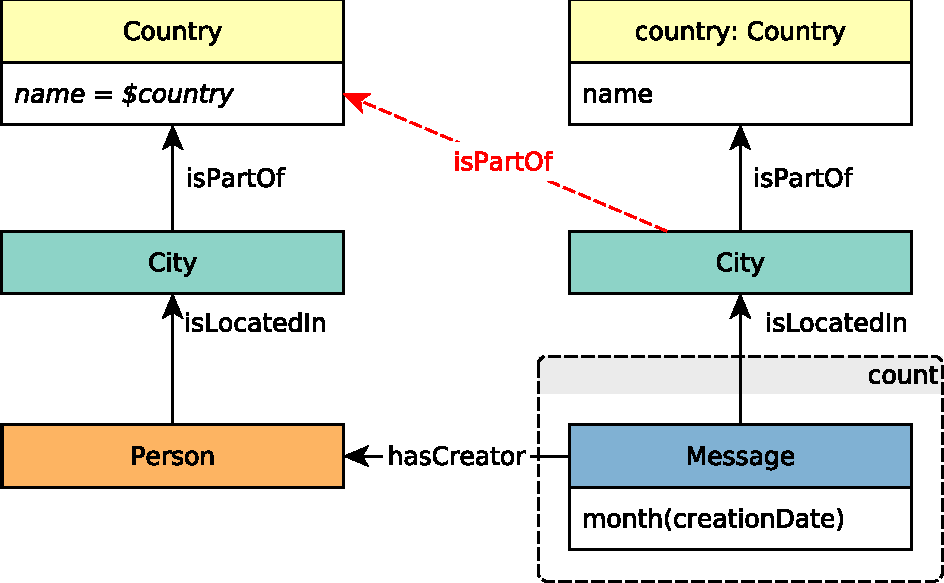
\includegraphics[scale=\patternscale,margin=0cm .2cm]{patterns/bi23}
		\caption{Example graph pattern.}
		\label{fig:example-graph-pattern}
	\end{center}
\end{figure}


\chapter{Interactive Workload}

\section{Choke Points}

The design of the interactive workload queries has been conceived around two
main aspects: realism and technological relevance.  While realism has been
assessed by looking at existing social networks and thinking about what
interesting functionalities a user might desire from them, technological
relevance has been achieved by identifying a set of choke points queries should
stress.  These choke points capture those critical operations, techniques or
technologies that  could significatively affect the performance of the queries.
The choke points can be summarized in the following list:

% http://wiki.ldbcouncil.org/display/TUC/Interactive+Choke+Points

\subsection{Aggregation Performance}

The queries generally have a top-$k$ order by and often a group by in
addition to this.  These offer multiple optimization opportunities.
The queries also often have distinct operators, \ie distinct friends
within two steps.  Collectively these are all set operations that may
be implemented with some combination of hash and sorting, possibly
exploiting ordering in the data itself.  The aggregates are not
limited to counts and sums.  For example string concatenation occurs
as an aggregate, testing possible user defined aggregate support.
There is a wide range of cardinalities in grouping, from low, \eg country, to high, \eg post.

\subsection{Join Performance}

Each graph traversal step is in principle a join.  The join patterns are
diverse, exercising both index- and hash-based operators.   Queries are designed
so as to reward judicious use of hash join by having patterns starting with one
entity, fetching many related entities and then testing how these are related
to a third entity, \eg posts of a user with a tag of a given type.

\subsection{Data Access Locality}

Graph problems are notoriously non-local.  However, when queries touch
any non-trivial fraction of a dataset, locality will emerge and can be
exploited, for example by vectored index access or by ordering data so
that that a merge join is possible.

\subsection{Expression Calculation}

Queries often have expressions, including conditional expressions.
This provides opportunities for vectoring and tests efficient
management of intermediate results.

\subsection{Correlated Subqueries}

The workload has many correlated subqueries, for example constructts
like x within two steps but not in one step, which would typically be
a correlated subquery with NOT EXISTS.  There are also scalar
subqueries with aggregation, for example returning the count of posts
satisfying a certain criteria.


\subsection{Parallelism and Concurrency}

All queries offer opportunities for parallelism.  This tests a wide
range of constructs, for example partitioned parallel variants of
group by and distinct.  An interactive workload will typically avoid
trivially parallelizable table scans.  Thus the opportunities that
exist must be captured by index based, navigational query plans.  The
choice of whether to parallelize or not is often left to run time and
will have to depend on the actual data seen in the execution, as
starting a parallel thread with too little to do is
counter-productive.


\subsection{Graph Specifics}

Graph problems are generally characterized by transitive properties
and the fact that neighboring vertices often have a large overlap in
their environments.  This makes cardinality estimation harder.  For
example, a query optimizer needs to recognize whether a relationship
has a tree or graph shape in order to make correct cardinality
estimations.  Further, there are problems aggregating properties over
a set of consecutive edges.  The workload contains business questions
dealing with paths and aggregates across paths, as well as the easier
case of determining a membership in a hierarchy with a transitive
part-of relation.


\section{Query Specifications}

\subsection{Complex Reads Query Descriptions}
\label{sub:queries}

%\renewcommand*{\arraystretch}{1.1}

\subsection*{Interactive / complex / 1}
\label{section:interactive-complex-read-01}

\noindent\begin{tabularx}{\queryCardWidth}{|>{\queryPropertyCell}p{\queryPropertyCellWidth}|X|}
	\hline
	query & Interactive / complex / 1 \\ \hline
%
	title & Friends with certain name
 \\ \hline
%
	pattern & \hfill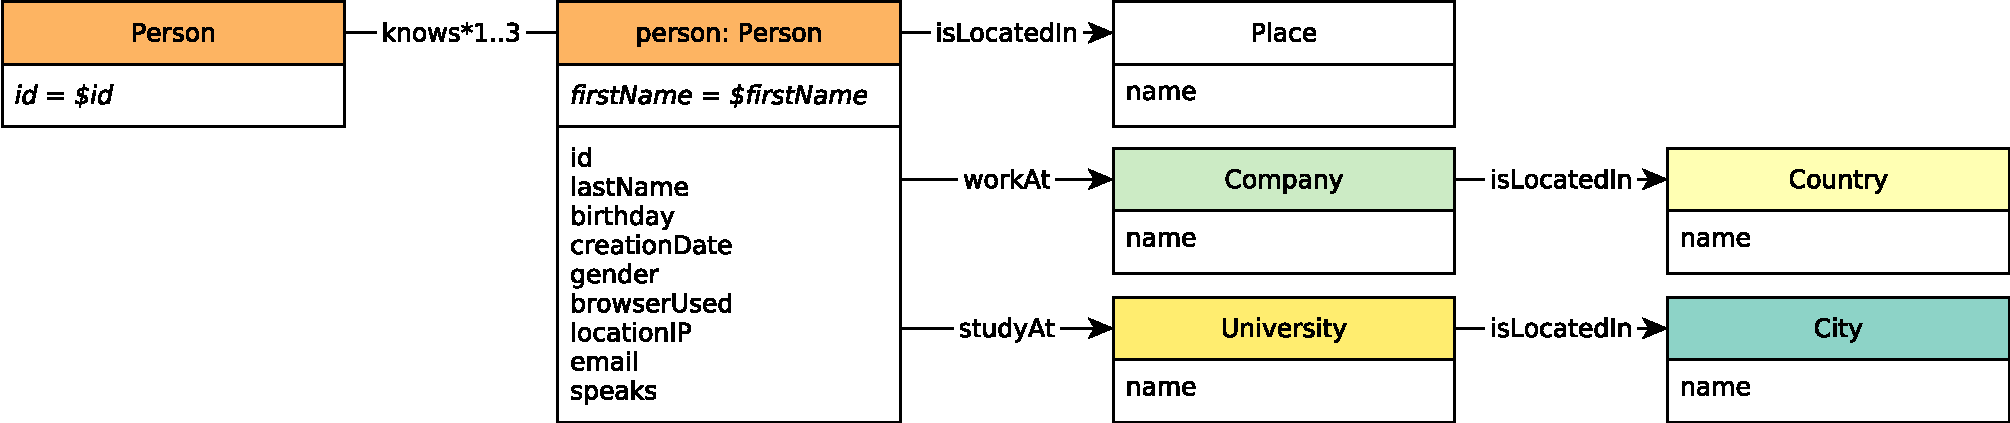
\includegraphics[scale=\patternscale,margin=0cm .2cm]{patterns/interactive-complex-read-01}\hfill\vadjust{} \\ \hline
%
	desc. & Given a start Person, find Persons with a given first name that the
start Person is connected to (excluding start Person) by at most 3 steps
via Knows relationships. Return Persons, including summaries of the
Persons workplaces and places of study.
 \\ \hline
%
	
		params &
		\innerCardVSpace{\begin{tabularx}{\attributeCardWidth}{|>{\paramNumberCell}c|>{\varNameCell}M|>{\typeCell}m{\typeWidth}|Y|} \hline
		$\mathsf{1}$ & Person.id
 & ID
 &  \\ \hline
		$\mathsf{2}$ & Person.firstName
 & String
 &  \\ \hline
		\end{tabularx}}\innerCardVSpace \\ \hline
	
%
	
		result &
		\innerCardVSpace{\begin{tabularx}{\attributeCardWidth}{|>{\resultNumberCell}c|>{\varNameCell}M|>{\typeCell}m{\typeWidth}|>{\resultOriginCell}c|Y|} \hline
		$\mathsf{1}$ & Person.id
 & ID
 & R &
				 \\ \hline
		$\mathsf{2}$ & Person.lastName
 & String
 & R &
				 \\ \hline
		$\mathsf{3}$ & Person.birthday
 & Date
 & R &
				 \\ \hline
		$\mathsf{4}$ & Person.creationDate
 & DateTime
 & R &
				 \\ \hline
		$\mathsf{5}$ & Person.gender
 & String
 & R &
				 \\ \hline
		$\mathsf{6}$ & Person.browserUsed
 & String
 & R &
				 \\ \hline
		$\mathsf{7}$ & Person.locationIP
 & String
 & R &
				 \\ \hline
		$\mathsf{8}$ & \{Person.email\}
 & \{String\}
 & R &
				 \\ \hline
		$\mathsf{9}$ & \{Person.speaks\}
 & \{String\}
 & R &
				 \\ \hline
		$\mathsf{10}$ & Person-isLocatedIn-\textgreater{}Place.name
 & String
 & R &
				 \\ \hline
		$\mathsf{11}$ & \{Person-studyAt-\textgreater{}University.name,
Person-studyAt-\textgreater{}.classYear,
Person-studyAt-\textgreater{}University-isLocatedIn-\textgreater{}City.name\}
 & \{\}
 & R &
				 \\ \hline
		$\mathsf{12}$ & \{Person-workAt-\textgreater{}Company.name,
Person-workAt-\textgreater{}.workFrom,
Person-workAt-\textgreater{}Company-isLocatedIn-\textgreater{}Country.name\}
 & \{\}
 & R &
				 \\ \hline
		\end{tabularx}}\innerCardVSpace \\ \hline
	
%
	
		sort		&
		\innerCardVSpace{\begin{tabularx}{\attributeCardWidth}{|>{\sortNumberCell}c|>{\varNameCell}M|>{\directionCell}c|Y|} \hline
		$\mathsf{1}$ & distanceFromPerson
 & $\asc
$ &  \\ \hline
		$\mathsf{2}$ & Person.lastName
 & $\asc
$ &  \\ \hline
		$\mathsf{3}$ & Person.id
 & $\asc
$ &  \\ \hline
		\end{tabularx}}\innerCardVSpace \\ \hline
	%
	limit & 20 \\ \hline
	%
	CPs &
	\multicolumn{1}{>{\raggedright}l|}{
		\chokePoint{1.3}, 
		\chokePoint{2.1}, 
		\chokePoint{5.3}
		} \\ \hline
	%
	relevance &
		\small This query is a representative of a simple navigational query. It looks for paths of length one, two or three through
the knows relation, starting from a given Person and ending at a Person with a given name. It is interesting for several
aspects. First, it requires for a complex aggregation, that is, returning the concatenation of universities, companies,
languages and email information of the person. Second, it tests the ability of the optimizer to move the evaluation of
sub-queries functionally dependant on the Person, after the evaluation of the top-k. Finally, performance is
highly sensitive to properly estimating the cardinalities in each transitive path, and paying attention not to explode
already visited Persons.
 \\ \hline%
\end{tabularx}
\queryCardVSpace
\renewcommand*{\arraystretch}{1.1}

\subsection*{Interactive / complex / 2}
\label{section:interactive-complex-read-02}

% change \emph{} to use sans-serif font
\let\oldemph\emph
\renewcommand{\emph}[1]{{\footnotesize \sf #1}}

\renewcommand{\currentQueryCard}{2}
\marginpar{
	\raggedleft
	\vspace{0.22ex}

	\queryRefCard{interactive-complex-read-01}{Interactive}{1}\\
	\queryRefCard{interactive-complex-read-02}{Interactive}{2}\\
	\queryRefCard{interactive-complex-read-03}{Interactive}{3}\\
	\queryRefCard{interactive-complex-read-04}{Interactive}{4}\\
	\queryRefCard{interactive-complex-read-05}{Interactive}{5}\\
	\queryRefCard{interactive-complex-read-06}{Interactive}{6}\\
	\queryRefCard{interactive-complex-read-07}{Interactive}{7}\\
	\queryRefCard{interactive-complex-read-08}{Interactive}{8}\\
	\queryRefCard{interactive-complex-read-09}{Interactive}{9}\\
	\queryRefCard{interactive-complex-read-10}{Interactive}{10}\\
	\queryRefCard{interactive-complex-read-11}{Interactive}{11}\\
	\queryRefCard{interactive-complex-read-12}{Interactive}{12}\\
	\queryRefCard{interactive-complex-read-13}{Interactive}{13}\\
	\queryRefCard{interactive-complex-read-14}{Interactive}{14}\\
}

\noindent\begin{tabularx}{\queryCardWidth}{|>{\queryPropertyCell}p{\queryPropertyCellWidth}|X|}
	\hline
	query & Interactive / complex / 2 \\ \hline
%
	title & Recent posts and comments by your friends \\ \hline
%
	pattern & \multicolumn{1}{c|}{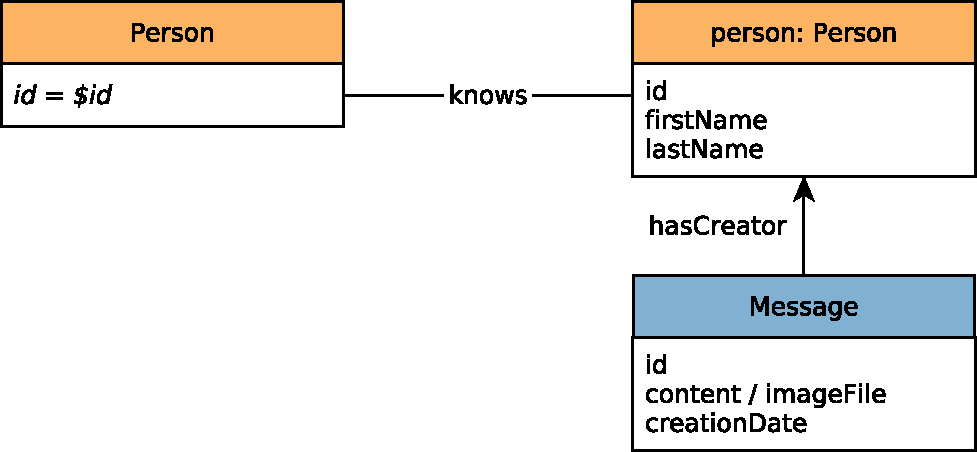
\includegraphics[scale=\patternscale,margin=0cm .2cm]{patterns/interactive-complex-read-02}} \\ \hline
%
	desc. & Given a start Person, find (most recent) Messages from all of that
Person's friends, that were created before (and including) a given date.
 \\ \hline
%
	
		params &
		\innerCardVSpace{\begin{tabularx}{\attributeCardWidth}{|>{\paramNumberCell}c|>{\varNameCell}M|>{\typeCell}m{\typeWidth}|Y|} \hline
		$\mathsf{1}$ & Person.id
 & ID
 &  \\ \hline
		$\mathsf{2}$ & date
 & DateTime
 &  \\ \hline
		\end{tabularx}}\innerCardVSpace \\ \hline
	
%
	
		result &
		\innerCardVSpace{\begin{tabularx}{\attributeCardWidth}{|>{\resultNumberCell}c|>{\varNameCell}M|>{\typeCell}m{\typeWidth}|>{\resultOriginCell}c|Y|} \hline
		$\mathsf{1}$ & Message-hasCreator-\textgreater{}Person.id & ID & R &
				 \\ \hline
		$\mathsf{2}$ & Message-hasCreator-\textgreater{}Person.firstName & String & R &
				 \\ \hline
		$\mathsf{3}$ & Message-hasCreator-\textgreater{}Person.lastName & String & R &
				 \\ \hline
		$\mathsf{4}$ & Message.id & ID & R &
				 \\ \hline
		$\mathsf{5}$ & Message.content or Post.imageFile & String & R &
				 \\ \hline
		$\mathsf{6}$ & Message.creationDate & DateTime & R &
				 \\ \hline
		\end{tabularx}}\innerCardVSpace \\ \hline
	
%
	
		sort		&
		\innerCardVSpace{\begin{tabularx}{\attributeCardWidth}{|>{\sortNumberCell}c|>{\varNameCell}M|>{\directionCell}c|Y|} \hline
		$\mathsf{1}$ & Message.creationDate
 & $\desc
$ &  \\ \hline
		$\mathsf{2}$ & Message.id
 & $\asc
$ &  \\ \hline
		\end{tabularx}}\innerCardVSpace \\ \hline
	%
	limit & 20 \\ \hline
	%
	CPs &
	\multicolumn{1}{>{\raggedright}l|}{
		\chokePoint{1.1}, 
		\chokePoint{2.2}, 
		\chokePoint{2.3}, 
		\chokePoint{3.2}
		} \\ \hline
	%
	relevance &
		\small This is a navigational query looking for paths of length two, starting from a given Person, going to their friends and
from them, moving to their published Posts and Comments. This query exercices both the optimizer and how data is
stored. It tests the ability to create execution plans taking advantage of the orderings induced by some operators to
avoid performing expensive sorts. This query requires selecting Posts and Comments based on their creation date,
which might be correlated with their identifier and therefore, having intermediate results with interesting orders.
Also, messages could be stored in an order correlated with their creation date to improve data access locality. Finally,
as many of the attributes required in the projection are not needed for the execution of the query, it is expected that
the query optimizer will move the projection to the end.
 \\ \hline%
\end{tabularx}
\queryCardVSpace

% change \emph back to the old one
\renewcommand{\emph}[1]{\oldemph{#1}}
\renewcommand*{\arraystretch}{1.1}

\subsection*{Interactive / complex / 3}
\label{section:interactive-complex-read-03}

% change \emph{} to use sans-serif font
\let\oldemph\emph
\renewcommand{\emph}[1]{{\footnotesize \sf #1}}

\renewcommand{\currentQueryCard}{3}
\marginpar{
	\raggedleft
	\vspace{0.22ex}

	\queryRefCard{interactive-complex-read-01}{IC}{1}\\
	\queryRefCard{interactive-complex-read-02}{IC}{2}\\
	\queryRefCard{interactive-complex-read-03}{IC}{3}\\
	\queryRefCard{interactive-complex-read-04}{IC}{4}\\
	\queryRefCard{interactive-complex-read-05}{IC}{5}\\
	\queryRefCard{interactive-complex-read-06}{IC}{6}\\
	\queryRefCard{interactive-complex-read-07}{IC}{7}\\
	\queryRefCard{interactive-complex-read-08}{IC}{8}\\
	\queryRefCard{interactive-complex-read-09}{IC}{9}\\
	\queryRefCard{interactive-complex-read-10}{IC}{10}\\
	\queryRefCard{interactive-complex-read-11}{IC}{11}\\
	\queryRefCard{interactive-complex-read-12}{IC}{12}\\
	\queryRefCard{interactive-complex-read-13}{IC}{13}\\
	\queryRefCard{interactive-complex-read-14}{IC}{14}\\
}


\noindent\begin{tabularx}{\queryCardWidth}{|>{\queryPropertyCell}p{\queryPropertyCellWidth}|X|}
	\hline
	query & Interactive / complex / 3 \\ \hline
%
	title & Friends and friends of friends that have been to countries X and Y \\ \hline
%
	pattern & \multicolumn{1}{c|}{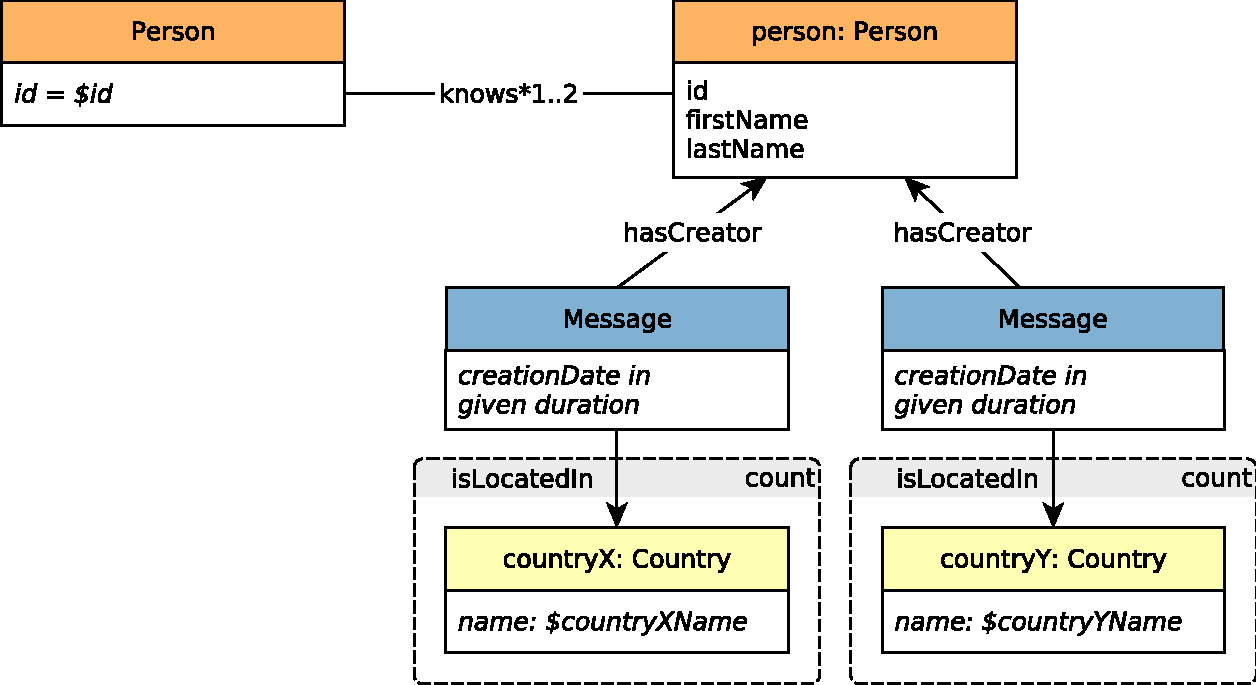
\includegraphics[scale=\patternscale,margin=0cm .2cm]{patterns/interactive-complex-read-03}} \\ \hline
%
	desc. & Given a start Person, find Persons that are their friends and friends of
friends (excluding start Person) that have made Posts/Comments in both
of the given Countries, X and Y, within a given period. Only Persons
that are foreign to Countries X and Y are considered, that is Persons
whose Location is not Country X or Country Y.
 \\ \hline
%
	
		params &
		\innerCardVSpace{\begin{tabularx}{\attributeCardWidth}{|>{\paramNumberCell}c|>{\varNameCell}M|>{\typeCell}m{\typeWidth}|Y|} \hline
		$\mathsf{1}$ & Person.id
 & ID
 &  \\ \hline
		$\mathsf{2}$ & CountryX.name
 & String
 &  \\ \hline
		$\mathsf{3}$ & CountryY.name
 & String
 &  \\ \hline
		$\mathsf{4}$ & startDate
 & Date
 & Beginning of requested period
 \\ \hline
		$\mathsf{5}$ & duration
 & 32-bit Integer
 & Duration of requested period, in days the interval {[}startDate,
startDate + Duration) is closed-open
 \\ \hline
		\end{tabularx}}\innerCardVSpace \\ \hline
	
%
	
		result &
		\innerCardVSpace{\begin{tabularx}{\attributeCardWidth}{|>{\resultNumberCell}c|>{\varNameCell}M|>{\typeCell}m{\typeWidth}|>{\resultOriginCell}c|Y|} \hline
		$\mathsf{1}$ & Person.id & ID & R &
				 \\ \hline
		$\mathsf{2}$ & Person.firstName & String & R &
				 \\ \hline
		$\mathsf{3}$ & Person.lastName & String & R &
				 \\ \hline
		$\mathsf{4}$ & countX & 32-bit Integer & A &
				Number of Messages from Country X made by Person within the given time
 \\ \hline
		$\mathsf{5}$ & countY & 32-bit Integer & A &
				Number of Messages from Country Y made by Person within the given time
 \\ \hline
		$\mathsf{6}$ & count & 32-bit Integer & A &
				\texttt{countX} + \texttt{countY}
 \\ \hline
		\end{tabularx}}\innerCardVSpace \\ \hline
	
%
	
		sort		&
		\innerCardVSpace{\begin{tabularx}{\attributeCardWidth}{|>{\sortNumberCell}c|>{\varNameCell}M|>{\directionCell}c|Y|} \hline
		$\mathsf{1}$ & countX
 & $\desc
$ &  \\ \hline
		$\mathsf{2}$ & Person.id
 & $\asc
$ &  \\ \hline
		\end{tabularx}}\innerCardVSpace \\ \hline
	%
	limit & 20 \\ \hline
	%
	CPs &
	\multicolumn{1}{>{\raggedright}l|}{
		\chokePoint{2.1}, 
		\chokePoint{3.1}, 
		\chokePoint{5.1}
		} \\ \hline
	%
	relevance &
		\small This query looks for paths of length two and three, starting from a Person, going to friends or friends of friends, and
then moving to Messages. This query tests the ability of the query optimizer to select the most efficient join ordering,
which will depend on the cardinalities of the intermediate results. Many friends of friends can be duplicate, then it is
expected to eliminate duplicates and those people prior to access the Post and Comments, as well as eliminate those
friends from countries X and Y, as the size of the intermediate results can be severely affected. A possible structural
optimization could be to materialize the number of Posts and Comments created by a person, and progressively
filter those people that could not even fall in the top 20 even having all their posts in the countries X and Y.
 \\ \hline%
\end{tabularx}
\queryCardVSpace

% change \emph back to the old one
\let\emph\oldemph
\renewcommand*{\arraystretch}{1.1}

\subsection*{Interactive / complex / 4}
\label{section:interactive-complex-read-04}

% change \emph{} to use sans-serif font
\let\oldemph\emph
\renewcommand{\emph}[1]{{\footnotesize \sf #1}}

\renewcommand{\currentQueryCard}{4}
\marginpar{
	\raggedleft
	\vspace{0.22ex}

	\queryRefCard{interactive-complex-read-01}{IC}{1}\\
	\queryRefCard{interactive-complex-read-02}{IC}{2}\\
	\queryRefCard{interactive-complex-read-03}{IC}{3}\\
	\queryRefCard{interactive-complex-read-04}{IC}{4}\\
	\queryRefCard{interactive-complex-read-05}{IC}{5}\\
	\queryRefCard{interactive-complex-read-06}{IC}{6}\\
	\queryRefCard{interactive-complex-read-07}{IC}{7}\\
	\queryRefCard{interactive-complex-read-08}{IC}{8}\\
	\queryRefCard{interactive-complex-read-09}{IC}{9}\\
	\queryRefCard{interactive-complex-read-10}{IC}{10}\\
	\queryRefCard{interactive-complex-read-11}{IC}{11}\\
	\queryRefCard{interactive-complex-read-12}{IC}{12}\\
	\queryRefCard{interactive-complex-read-13}{IC}{13}\\
	\queryRefCard{interactive-complex-read-14}{IC}{14}\\
}


\noindent\begin{tabularx}{\queryCardWidth}{|>{\queryPropertyCell}p{\queryPropertyCellWidth}|X|}
	\hline
	query & Interactive / complex / 4 \\ \hline
%
	title & New topics \\ \hline
%
	pattern & \multicolumn{1}{c|}{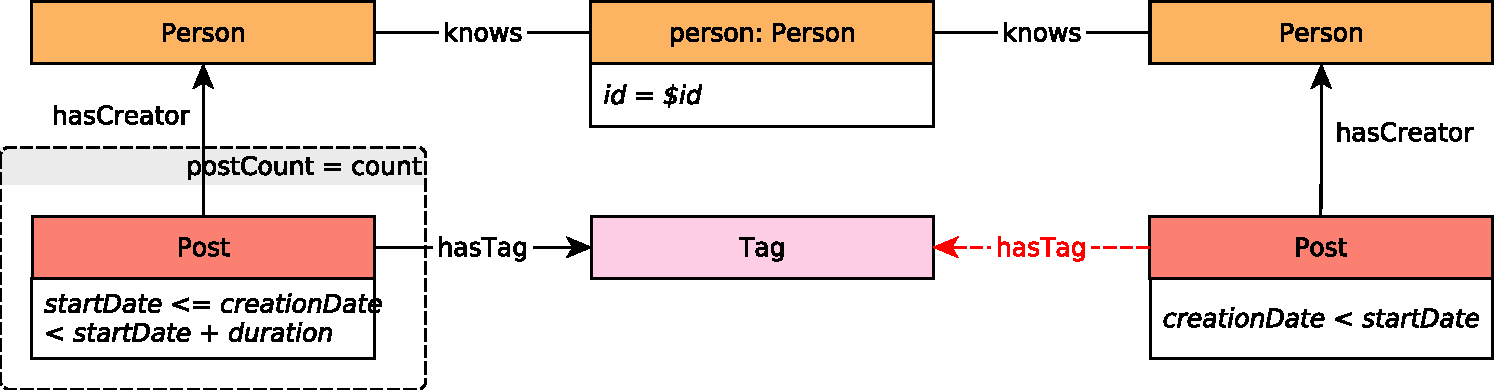
\includegraphics[scale=\patternscale,margin=0cm .2cm]{patterns/interactive-complex-read-04}} \\ \hline
%
	desc. & Given a start Person, find Tags that are attached to Posts that were
created by that Person's friends. Only include Tags that were attached
to friends' Posts created within a given time interval, and that were
never attached to friends' Posts created before this interval.
 \\ \hline
%
	
		params &
		\innerCardVSpace{\begin{tabularx}{\attributeCardWidth}{|>{\paramNumberCell}c|>{\varNameCell}M|>{\typeCell}m{\typeWidth}|Y|} \hline
		$\mathsf{1}$ & Person.id
 & ID
 &  \\ \hline
		$\mathsf{2}$ & startDate
 & Date
 &  \\ \hline
		$\mathsf{3}$ & duration
 & 32-bit Integer
 & Duration of requested period, in days the interval {[}startDate,
startDate + Duration) is closed-open
 \\ \hline
		\end{tabularx}}\innerCardVSpace \\ \hline
	
%
	
		result &
		\innerCardVSpace{\begin{tabularx}{\attributeCardWidth}{|>{\resultNumberCell}c|>{\varNameCell}M|>{\typeCell}m{\typeWidth}|>{\resultOriginCell}c|Y|} \hline
		$\mathsf{1}$ & Tag.name & String & R &
				 \\ \hline
		$\mathsf{2}$ & count & 32-bit Integer & A &
				Number of Posts made within the given time interval that have this Tag
 \\ \hline
		\end{tabularx}}\innerCardVSpace \\ \hline
	
%
	
		sort		&
		\innerCardVSpace{\begin{tabularx}{\attributeCardWidth}{|>{\sortNumberCell}c|>{\varNameCell}M|>{\directionCell}c|Y|} \hline
		$\mathsf{1}$ & count
 & $\desc
$ &  \\ \hline
		$\mathsf{2}$ & Tag.name
 & $\asc
$ &  \\ \hline
		\end{tabularx}}\innerCardVSpace \\ \hline
	%
	limit & 10 \\ \hline
	%
	CPs &
	\multicolumn{1}{>{\raggedright}l|}{
		\chokePoint{2.3}
		} \\ \hline
	%
	relevance &
		\small This query looks for paths of length two, starting from a given Person, moving to Posts and then to Tags. It tests
the ability of the query optimizer to properly select the usage of hash joins or index based joins, depending on the
cardinality of the intermediate results. These cardinalities are clearly affected by the input Person, the number of
friends, the variety of Tags, the time interval and the number of Posts.
 \\ \hline%
\end{tabularx}
\queryCardVSpace

% change \emph back to the old one
\let\emph\oldemph
\renewcommand*{\arraystretch}{1.1}

\subsection*{Interactive / complex / 5}
\label{section:interactive-complex-read-05}

% change \emph{} to use sans-serif font
\let\oldemph\emph
\renewcommand{\emph}[1]{{\footnotesize \sf #1}}

\renewcommand{\currentQueryCard}{5}
\input{query-cards/interactive-navbar}

\noindent\begin{tabularx}{\queryCardWidth}{|>{\queryPropertyCell}p{\queryPropertyCellWidth}|X|}
	\hline
	query & Interactive / complex / 5 \\ \hline
%
	title & New groups
 \\ \hline
%
	pattern & \hfill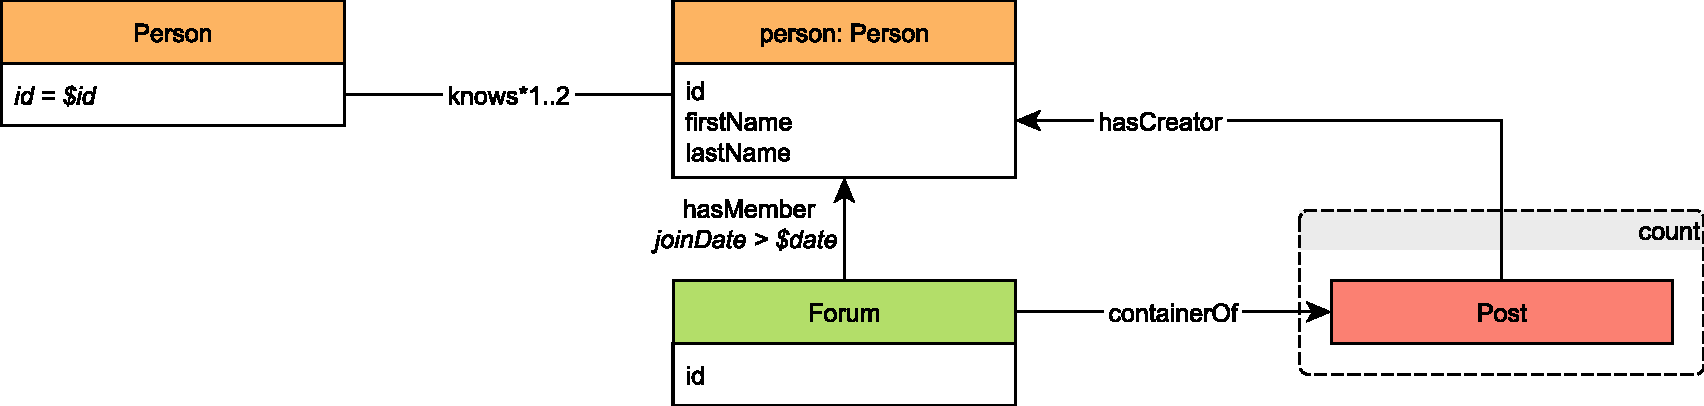
\includegraphics[scale=\patternscale,margin=0cm .2cm]{patterns/interactive-complex-read-05}\hfill\vadjust{} \\ \hline
%
	desc. & Given a start Person, find the Forums which that Person's friends and
friends of friends (excluding start Person) became Members of after a
given date. For each forum find the number of Posts that were created by
any of these Persons. For each Forum and consider only those Persons
which joined that particular Forum after the given date.
 \\ \hline
%
	
		params &
		\innerCardVSpace{\begin{tabularx}{\attributeCardWidth}{|>{\paramNumberCell}c|>{\varNameCell}M|>{\typeCell}m{\typeWidth}|Y|} \hline
		$\mathsf{1}$ & Person.id
 & ID
 &  \\ \hline
		$\mathsf{2}$ & date
 & Date
 &  \\ \hline
		\end{tabularx}}\innerCardVSpace \\ \hline
	
%
	
		result &
		\innerCardVSpace{\begin{tabularx}{\attributeCardWidth}{|>{\resultNumberCell}c|>{\varNameCell}M|>{\typeCell}m{\typeWidth}|>{\resultOriginCell}c|Y|} \hline
		$\mathsf{1}$ & Forum.title & String & R &
				 \\ \hline
		$\mathsf{2}$ & count & 32-bit Integer & A &
				Number of Posts made in Forum that were created by friends
 \\ \hline
		\end{tabularx}}\innerCardVSpace \\ \hline
	
%
	
		sort		&
		\innerCardVSpace{\begin{tabularx}{\attributeCardWidth}{|>{\sortNumberCell}c|>{\varNameCell}M|>{\directionCell}c|Y|} \hline
		$\mathsf{1}$ & count
 & $\desc
$ &  \\ \hline
		$\mathsf{2}$ & Forum.id
 & $\asc
$ &  \\ \hline
		\end{tabularx}}\innerCardVSpace \\ \hline
	%
	limit & 20 \\ \hline
	%
	CPs &
	\multicolumn{1}{>{\raggedright}l|}{
		\chokePoint{2.3}, 
		\chokePoint{3.3}
		} \\ \hline
	%
	relevance &
		\small This query looks for paths of length two and three, starting from a given Person, moving to friends and friends of
friends, and then getting the Forums they are members of. Besides testing the ability of the query optimizer to select
the proper join operator, it rewards the usage of indexes, but their accesses will be presumably scattered due to the
two/three-hop search space of the query, leading to unpredictable and scattered index accesses. Having efficient
implementations of such indexes will be highly beneficial.
 \\ \hline%
\end{tabularx}
\queryCardVSpace

% change \emph back to the old one
\renewcommand{\emph}[1]{\oldemph{#1}}
\renewcommand*{\arraystretch}{1.1}

\label{sec:interactive-complex-read-06}
\noindent\begin{tabularx}{\queryCardWidth}{|>{\queryPropertyCell}c|X|}
	\hline
	query & Interactive / complex / 6 \\ \hline
%
	title & Tag co-occurrence \\ \hline
%
    pattern & \hfill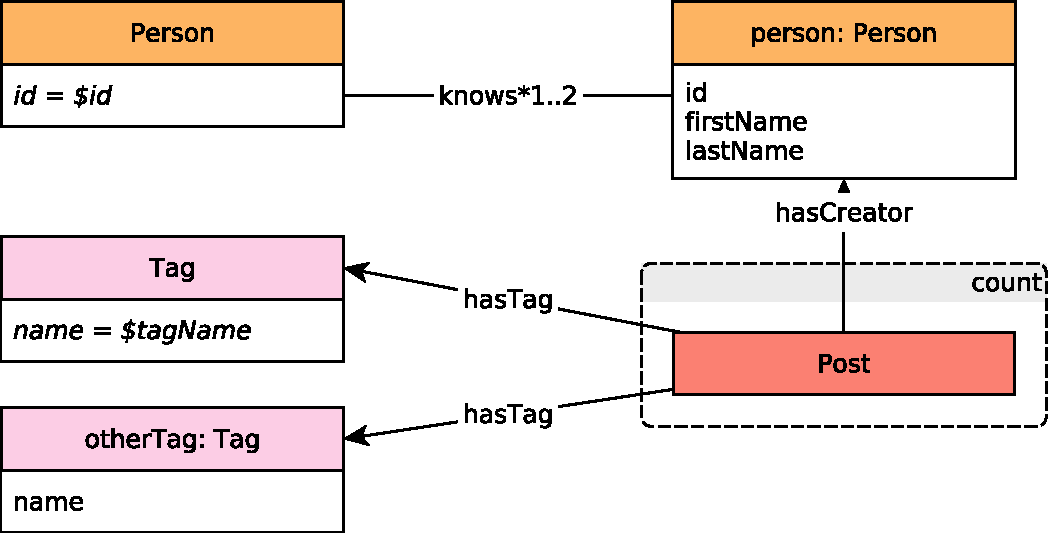
\includegraphics[scale=\patternscale,margin=0cm .2cm]{patterns/interactive-complex-read-06}\hfill\vadjust{} \\ \hline
%
	desc. & Given a start Person and some Tag, find the other Tags that occur
together with this Tag on Posts that were created by start Person's
friends and friends of friends (excluding start Person). Return For each
Tag, find the count of Posts that were created by these Persons, which
contain both this Tag and the given Tag.
 \\ \hline
%
	
%
    
        params &
        \innerCardVSpace{\begin{tabularx}{\attributeCardWidth}{|>{\paramNumberCell}c|>{\varNameCell}M|>{\typeCell}m{\typeWidth}|Y|} \hline
        \cellcolor{parameter} \color{white} \footnotesize $\mathsf{1}$ &Person.id& ID &  \\ \hline
        \cellcolor{parameter} \color{white} \footnotesize $\mathsf{2}$ &Tag.name& String &  \\ \hline
        \end{tabularx}}\innerCardVSpace \\ \hline
	
%
	
        result &
        \innerCardVSpace{\begin{tabularx}{\attributeCardWidth}{|>{\resultNumberCell}c|>{\varNameCell}M|>{\typeCell}m{\typeWidth}|>{\resultOriginCell}c|Y|} \hline
        $\mathsf{1}$ & Tag.name & String &R&
                 \\ \hline
        $\mathsf{2}$ & count & 32-bit Integer &A&
                number of Posts that were created by friends and friends of friends, which contain this Tag \\ \hline
        \end{tabularx}}\innerCardVSpace \\ \hline
	
%
	sort        &
        \innerCardVSpace{\begin{tabular}{|>{\sortNumberCell}c|>{\varNameCell}l|>{\directionCell}c|} \hline
        $\mathsf{1}$ & count & $\desc$ \\ \hline
        $\mathsf{2}$ & Tag.name & $\asc$ \\ \hline
        \end{tabular}}\innerCardVSpace \\ \hline
	%
	limit & 10 \\ \hline
	%
	CPs &
	\multicolumn{1}{>{\raggedright}l|}{
	    \chokePoint{5.1}
	    } \\ \hline
	%
    relevance &
        \small This query looks for paths of lengths three or four, starting from a Given Person, moving to friends or friends of
friends, then to Posts and finally ending at a given Tag.
 \\ \hline%
\end{tabularx}
\queryCardVSpace
\renewcommand*{\arraystretch}{1.1}

\subsection*{Interactive / complex / 7}
\label{section:interactive-complex-read-07}

\noindent\begin{tabularx}{\queryCardWidth}{|>{\queryPropertyCell}p{\queryPropertyCellWidth}|X|}
	\hline
	query & Interactive / complex / 7 \\ \hline
%
	title & Recent likers
 \\ \hline
%
	pattern & \hfill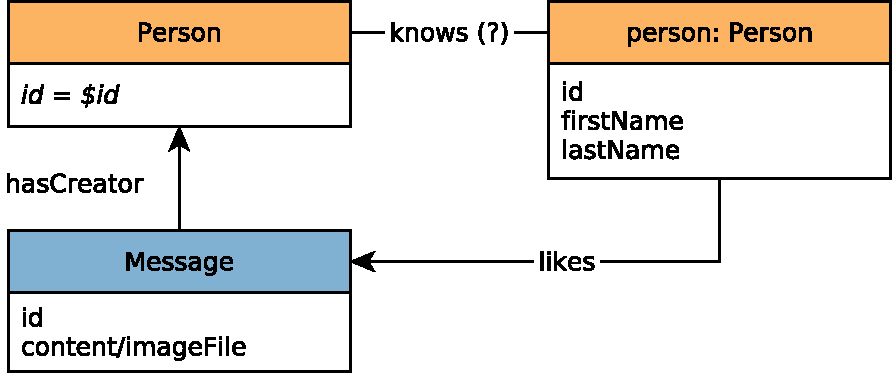
\includegraphics[scale=\patternscale,margin=0cm .2cm]{patterns/interactive-complex-read-07}\hfill\vadjust{} \\ \hline
%
	desc. & Given a start Person, find (most recent) Likes on any of start Person's
Messages. Find Persons that Liked any of start Person's Messages, the
Messages they liked most recently, creation date of that Like, and the
latency (in minutes) between creation of Messages and Like.
Additionally, for each Person found return a flag indicating whether the
liker is a friend of start Person. In the case that a Person Liked
multiple Messages at the same time, return the Message with lowest
identifier.
 \\ \hline
%
	
		params &
		\innerCardVSpace{\begin{tabularx}{\attributeCardWidth}{|>{\paramNumberCell}c|>{\varNameCell}M|>{\typeCell}m{\typeWidth}|Y|} \hline
		$\mathsf{1}$ & Person.id
 & 64-bit Integer
 &  \\ \hline
		\end{tabularx}}\innerCardVSpace \\ \hline
	
%
	
		result &
		\innerCardVSpace{\begin{tabularx}{\attributeCardWidth}{|>{\resultNumberCell}c|>{\varNameCell}M|>{\typeCell}m{\typeWidth}|>{\resultOriginCell}c|Y|} \hline
		$\mathsf{1}$ & Person.id
 & ID
 & R &
				 \\ \hline
		$\mathsf{2}$ & Person.firstName
 & String
 & R &
				 \\ \hline
		$\mathsf{3}$ & Person.lastName
 & String
 & R &
				 \\ \hline
		$\mathsf{4}$ & Like.creationDate
 & DateTime
 & R &
				 \\ \hline
		$\mathsf{5}$ & Message.id
 & ID
 & R &
				 \\ \hline
		$\mathsf{6}$ & Message.content or Post.imageFile
 & String
 & R &
				 \\ \hline
		$\mathsf{7}$ & latency
 & 32-bit Integer
 & R &
				Duration between creation of Message and Like, in minutes
 \\ \hline
		$\mathsf{8}$ & isNew
 & Boolean
 & R &
				\texttt{false} if liker Person is friend of start Person, \texttt{true}
otherwise
 \\ \hline
		\end{tabularx}}\innerCardVSpace \\ \hline
	
%
	
		sort		&
		\innerCardVSpace{\begin{tabularx}{\attributeCardWidth}{|>{\sortNumberCell}c|>{\varNameCell}M|>{\directionCell}c|Y|} \hline
		$\mathsf{1}$ & Like.creationDate
 & $\desc
$ &  \\ \hline
		$\mathsf{2}$ & Person.id
 & $\asc
$ &  \\ \hline
		\end{tabularx}}\innerCardVSpace \\ \hline
	%
	limit & 20 \\ \hline
	%
	CPs &
	\multicolumn{1}{>{\raggedright}l|}{
		\chokePoint{2.2}, 
		\chokePoint{2.3}, 
		\chokePoint{3.3}, 
		\chokePoint{5.1}
		} \\ \hline
	%
	relevance &
		\small This query looks for paths of length two, starting from a given Person, moving
to its published messages and then to Persons who liked them. It tests several aspects related to join optimization,
both at query optimization plan level and execution engine level. On the one hand, many of the columns needed for
the projection are only needed in the last stages of the query, so the optimizer is expected to delay the projection
until the end. This query implies accessing 2-hop data, and as a consequence, index accesses are expected to be
scattered. We expect to observe variate cardinalities, depending on the characteristics of the input parameter, so
properly selecting the join operators will be crucial. This query has a lot of correlated sub-queries, so it is testing
the ability to flatten the query execution plans.
 \\ \hline%
\end{tabularx}
\queryCardVSpace
\renewcommand*{\arraystretch}{1.1}

\subsection*{Interactive / complex / 8}
\label{section:interactive-complex-read-08}

% change \emph{} to use sans-serif font
\let\oldemph\emph
\renewcommand{\emph}[1]{{\footnotesize \sf #1}}

\renewcommand{\currentQueryCard}{8}
\marginpar{
	\raggedleft
	\vspace{0.22ex}

	\queryRefCard{interactive-complex-read-01}{IC}{1}\\
	\queryRefCard{interactive-complex-read-02}{IC}{2}\\
	\queryRefCard{interactive-complex-read-03}{IC}{3}\\
	\queryRefCard{interactive-complex-read-04}{IC}{4}\\
	\queryRefCard{interactive-complex-read-05}{IC}{5}\\
	\queryRefCard{interactive-complex-read-06}{IC}{6}\\
	\queryRefCard{interactive-complex-read-07}{IC}{7}\\
	\queryRefCard{interactive-complex-read-08}{IC}{8}\\
	\queryRefCard{interactive-complex-read-09}{IC}{9}\\
	\queryRefCard{interactive-complex-read-10}{IC}{10}\\
	\queryRefCard{interactive-complex-read-11}{IC}{11}\\
	\queryRefCard{interactive-complex-read-12}{IC}{12}\\
	\queryRefCard{interactive-complex-read-13}{IC}{13}\\
	\queryRefCard{interactive-complex-read-14}{IC}{14}\\
}


\noindent\begin{tabularx}{\queryCardWidth}{|>{\queryPropertyCell}p{\queryPropertyCellWidth}|X|}
	\hline
	query & Interactive / complex / 8 \\ \hline
%
	title & Recent replies \\ \hline
%
	pattern & \centering 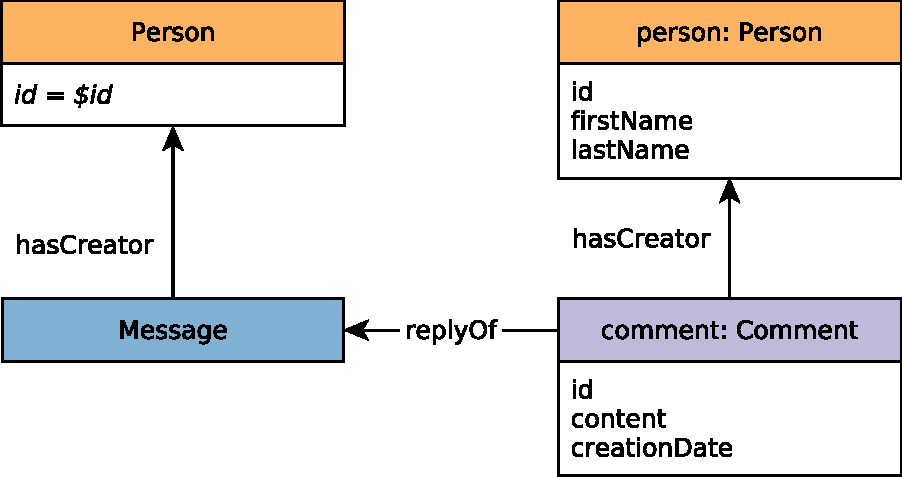
\includegraphics[scale=\patternscale,margin=0cm .2cm]{patterns/interactive-complex-read-08} \tabularnewline \hline
%
	desc. & Given a start \emph{Person}, find (most recent) \emph{Comments} that are
replies to \emph{Messages} of the start \emph{Person}. Only consider
direct (single-hop) replies, not the transitive (multi-hop) ones. Return
the reply \emph{Comments}, and the \emph{Person} that created each reply
\emph{Comment}.
 \\ \hline
%
	
		params &
		\innerCardVSpace{\begin{tabularx}{\attributeCardWidth}{|>{\paramNumberCell}c|>{\varNameCell}M|>{\typeCell}m{\typeWidth}|Y|} \hline
		$\mathsf{1}$ & Person.id
 & ID
 & \texttt{personId}
 \\ \hline
		\end{tabularx}}\innerCardVSpace \\ \hline
	
%
	
		result &
		\innerCardVSpace{\begin{tabularx}{\attributeCardWidth}{|>{\resultNumberCell}c|>{\varNameCell}M|>{\typeCell}m{\typeWidth}|>{\resultOriginCell}c|Y|} \hline
		$\mathsf{1}$ & Person.id & ID & R &
				\texttt{personId}
 \\ \hline
		$\mathsf{2}$ & Person.firstName & String & R &
				\texttt{personFirstName}
 \\ \hline
		$\mathsf{3}$ & Person.lastName & String & R &
				\texttt{personLastName}
 \\ \hline
		$\mathsf{4}$ & Comment.creationDate & DateTime & R &
				\texttt{commentCreationDate}
 \\ \hline
		$\mathsf{5}$ & Comment.id & ID & R &
				\texttt{commentId}
 \\ \hline
		$\mathsf{6}$ & Comment.content & String & R &
				\texttt{commentContent}
 \\ \hline
		\end{tabularx}}\innerCardVSpace \\ \hline
	
%
	
		sort		&
		\innerCardVSpace{\begin{tabularx}{\attributeCardWidth}{|>{\sortNumberCell}c|>{\varNameCell}M|>{\directionCell}c|Y|} \hline
		$\mathsf{1}$ & Comment.creationDate
 & $\desc
$ &  \\ \hline
		$\mathsf{2}$ & Comment.id
 & $\asc
$ &  \\ \hline
		\end{tabularx}}\innerCardVSpace \\ \hline
	%
	limit & 20 \\ \hline
	%
	CPs &
	\multicolumn{1}{>{\raggedright}l|}{
		\chokePoint{2.4}, 
		\chokePoint{3.2}, 
		\chokePoint{3.3}, 
		\chokePoint{5.3}
		} \\ \hline
	%
	relevance &
		\footnotesize This query looks for paths of length two, starting from a given
\emph{Person}, going through its created \emph{Messages} and finishing
at their replies. In this query there is temporal locality between the
replies being accessed. Thus the top-k order by this can interact with
the selection, i.e.~do not consider older \emph{Posts} than the 20th
oldest seen so far.
 \\ \hline%
\end{tabularx}
\queryCardVSpace

% change \emph back to the old one
\let\emph\oldemph
\renewcommand*{\arraystretch}{1.1}

\subsection*{Interactive / complex / 9}
\label{section:interactive-complex-read-09}

% change \emph{} to use sans-serif font
\let\oldemph\emph
\renewcommand{\emph}[1]{{\footnotesize \sf #1}}

\renewcommand{\currentQueryCard}{9}
\marginpar{
	\raggedleft
	\vspace{0.22ex}

	\queryRefCard{interactive-complex-read-01}{IC}{1}\\
	\queryRefCard{interactive-complex-read-02}{IC}{2}\\
	\queryRefCard{interactive-complex-read-03}{IC}{3}\\
	\queryRefCard{interactive-complex-read-04}{IC}{4}\\
	\queryRefCard{interactive-complex-read-05}{IC}{5}\\
	\queryRefCard{interactive-complex-read-06}{IC}{6}\\
	\queryRefCard{interactive-complex-read-07}{IC}{7}\\
	\queryRefCard{interactive-complex-read-08}{IC}{8}\\
	\queryRefCard{interactive-complex-read-09}{IC}{9}\\
	\queryRefCard{interactive-complex-read-10}{IC}{10}\\
	\queryRefCard{interactive-complex-read-11}{IC}{11}\\
	\queryRefCard{interactive-complex-read-12}{IC}{12}\\
	\queryRefCard{interactive-complex-read-13}{IC}{13}\\
	\queryRefCard{interactive-complex-read-14}{IC}{14}\\
}


\noindent\begin{tabularx}{\queryCardWidth}{|>{\queryPropertyCell}p{\queryPropertyCellWidth}|X|}
	\hline
	query & Interactive / complex / 9 \\ \hline
%
	title & Recent posts and comments by friends or friends of friends \\ \hline
%
	pattern & \multicolumn{1}{c|}{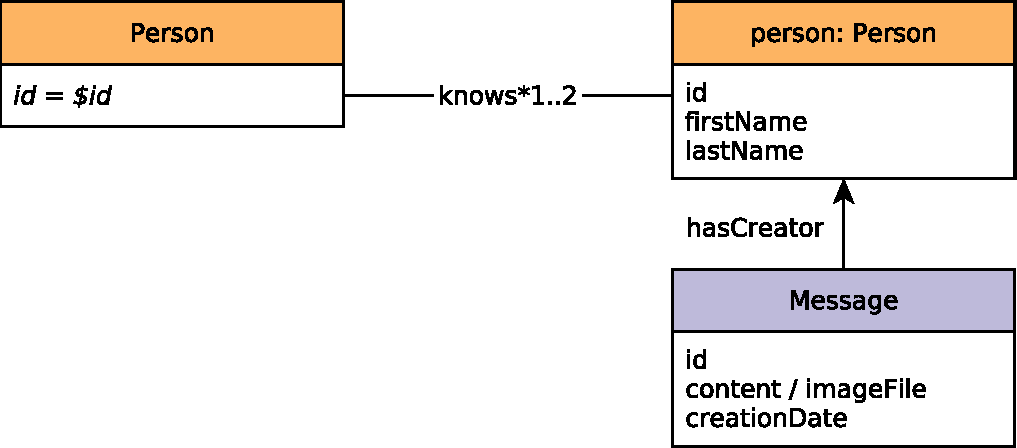
\includegraphics[scale=\patternscale,margin=0cm .2cm]{patterns/interactive-complex-read-09}} \\ \hline
%
	desc. & Given a start Person, find the (most recent) Messages created by that
Person's friends or friends of friends (excluding start Person). Only
consider the Messages created before a given date (excluding that date).
 \\ \hline
%
	
		params &
		\innerCardVSpace{\begin{tabularx}{\attributeCardWidth}{|>{\paramNumberCell}c|>{\varNameCell}M|>{\typeCell}m{\typeWidth}|Y|} \hline
		$\mathsf{1}$ & Person.id
 & ID
 &  \\ \hline
		$\mathsf{2}$ & date
 & Date
 &  \\ \hline
		\end{tabularx}}\innerCardVSpace \\ \hline
	
%
	
		result &
		\innerCardVSpace{\begin{tabularx}{\attributeCardWidth}{|>{\resultNumberCell}c|>{\varNameCell}M|>{\typeCell}m{\typeWidth}|>{\resultOriginCell}c|Y|} \hline
		$\mathsf{1}$ & Message-hasCreator-\textgreater{}Person.id & ID & R &
				\texttt{personId}
 \\ \hline
		$\mathsf{2}$ & Message-hasCreator-\textgreater{}Person.firstName & String & R &
				\texttt{personFirstName}
 \\ \hline
		$\mathsf{3}$ & Message-hasCreator-\textgreater{}Person.lastName & String & R &
				\texttt{personLastName}
 \\ \hline
		$\mathsf{4}$ & Message.id & ID & R &
				\texttt{commentOrPostId}
 \\ \hline
		$\mathsf{5}$ & Message.content or Post.imageFile & String & R &
				\texttt{commentOrPostContent}
 \\ \hline
		$\mathsf{6}$ & Message.creationDate & DateTime & R &
				\texttt{commentOrPostCreationDate}
 \\ \hline
		\end{tabularx}}\innerCardVSpace \\ \hline
	
%
	
		sort		&
		\innerCardVSpace{\begin{tabularx}{\attributeCardWidth}{|>{\sortNumberCell}c|>{\varNameCell}M|>{\directionCell}c|Y|} \hline
		$\mathsf{1}$ & Message.creationDate
 & $\desc
$ &  \\ \hline
		$\mathsf{2}$ & Message.id
 & $\asc
$ &  \\ \hline
		\end{tabularx}}\innerCardVSpace \\ \hline
	%
	limit & 20 \\ \hline
	%
	CPs &
	\multicolumn{1}{>{\raggedright}l|}{
		\chokePoint{1.1}, 
		\chokePoint{1.2}, 
		\chokePoint{2.2}, 
		\chokePoint{2.3}, 
		\chokePoint{3.2}, 
		\chokePoint{3.3}
		} \\ \hline
	%
	relevance &
		\footnotesize This query looks for paths of length two or three, starting from a given Person, moving to its friends and friends of
friends, and ending at their created Messages. This is one of the most complex queries, as the list of choke-points
indicates. This query is expected to touch variable amounts of data with entities of different characteristics, and
therefore, properly estimating cardinalities and selecting the proper operators will be crucial.
 \\ \hline%
\end{tabularx}
\queryCardVSpace

% change \emph back to the old one
\let\emph\oldemph
\renewcommand*{\arraystretch}{1.1}

\subsection*{Interactive / complex / 10}
\label{section:interactive-complex-read-10}

% change \emph{} to use sans-serif font
\let\oldemph\emph
\renewcommand{\emph}[1]{{\footnotesize \sf #1}}

\renewcommand{\currentQueryCard}{10}
\marginpar{
	\raggedleft
	\vspace{0.22ex}

	\queryRefCard{interactive-complex-read-01}{Interactive}{1}\\
	\queryRefCard{interactive-complex-read-02}{Interactive}{2}\\
	\queryRefCard{interactive-complex-read-03}{Interactive}{3}\\
	\queryRefCard{interactive-complex-read-04}{Interactive}{4}\\
	\queryRefCard{interactive-complex-read-05}{Interactive}{5}\\
	\queryRefCard{interactive-complex-read-06}{Interactive}{6}\\
	\queryRefCard{interactive-complex-read-07}{Interactive}{7}\\
	\queryRefCard{interactive-complex-read-08}{Interactive}{8}\\
	\queryRefCard{interactive-complex-read-09}{Interactive}{9}\\
	\queryRefCard{interactive-complex-read-10}{Interactive}{10}\\
	\queryRefCard{interactive-complex-read-11}{Interactive}{11}\\
	\queryRefCard{interactive-complex-read-12}{Interactive}{12}\\
	\queryRefCard{interactive-complex-read-13}{Interactive}{13}\\
	\queryRefCard{interactive-complex-read-14}{Interactive}{14}\\
}

\noindent\begin{tabularx}{\queryCardWidth}{|>{\queryPropertyCell}p{\queryPropertyCellWidth}|X|}
	\hline
	query & Interactive / complex / 10 \\ \hline
%
	title & Friend recommendation \\ \hline
%
	pattern & \multicolumn{1}{c|}{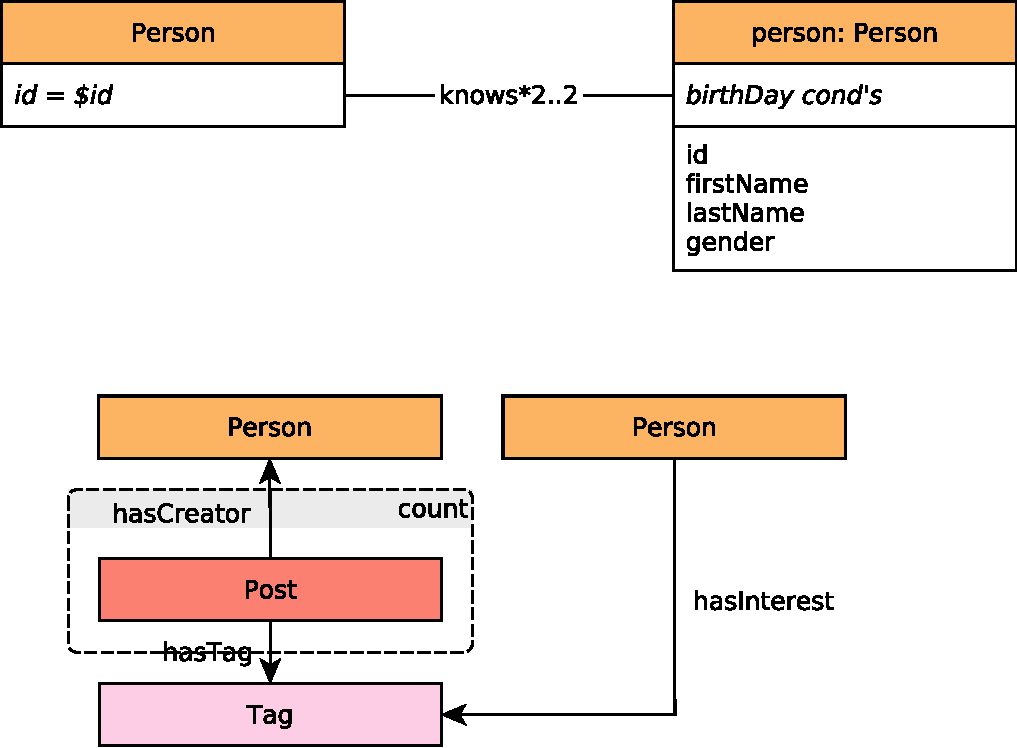
\includegraphics[scale=\patternscale,margin=0cm .2cm]{patterns/interactive-complex-read-10}} \\ \hline
%
	desc. & Given a start Person, find that Person's friends of friends (excluding
start Person, and immediate friends), who were born on or after the 21st
of a given month (in any year) and before the 22nd of the following
month. Calculate the similarity between each of these Persons and start
Person, where similarity for any Person is defined as follows:

\begin{itemize}
\tightlist
\item
  common = number of Posts created by that Person, such that the Post
  has a Tag that start Person is Interested in
\item
  uncommon = number of Posts created by that Person, such that the Post
  has no Tag that start Person is Interested in
\item
  similarity = common - uncommon
\end{itemize}
 \\ \hline
%
	
		params &
		\innerCardVSpace{\begin{tabularx}{\attributeCardWidth}{|>{\paramNumberCell}c|>{\varNameCell}M|>{\typeCell}m{\typeWidth}|Y|} \hline
		$\mathsf{1}$ & Person.id
 & ID
 &  \\ \hline
		$\mathsf{2}$ & month
 & 32-bit Integer
 & Between 1-12
 \\ \hline
		\end{tabularx}}\innerCardVSpace \\ \hline
	
%
	
		result &
		\innerCardVSpace{\begin{tabularx}{\attributeCardWidth}{|>{\resultNumberCell}c|>{\varNameCell}M|>{\typeCell}m{\typeWidth}|>{\resultOriginCell}c|Y|} \hline
		$\mathsf{1}$ & Person.id & ID & R &
				 \\ \hline
		$\mathsf{2}$ & Person.firstName & String & R &
				 \\ \hline
		$\mathsf{3}$ & Person.lastName & String & R &
				 \\ \hline
		$\mathsf{4}$ & similarity & 32-bit Integer & C &
				 \\ \hline
		$\mathsf{5}$ & Person.gender & String & R &
				 \\ \hline
		$\mathsf{6}$ & Person-isLocatedIn-\textgreater{}Place.name & String & R &
				 \\ \hline
		\end{tabularx}}\innerCardVSpace \\ \hline
	
%
	
		sort		&
		\innerCardVSpace{\begin{tabularx}{\attributeCardWidth}{|>{\sortNumberCell}c|>{\varNameCell}M|>{\directionCell}c|Y|} \hline
		$\mathsf{1}$ & similarity
 & $\desc
$ &  \\ \hline
		$\mathsf{2}$ & Person.id
 & $\asc
$ &  \\ \hline
		\end{tabularx}}\innerCardVSpace \\ \hline
	%
	limit & 10 \\ \hline
	%
	CPs &
	\multicolumn{1}{>{\raggedright}l|}{
		\chokePoint{2.3}, 
		\chokePoint{3.3}, 
		\chokePoint{4.1}, 
		\chokePoint{4.2}, 
		\chokePoint{5.1}, 
		\chokePoint{5.2}, 
		\chokePoint{6.1}, 
		\chokePoint{7.1}
		} \\ \hline
	%
	relevance &
		\small This query looks for paths of length two, starting from a Person and ending at the friends of their friends. It does
widely scattered graph traversal, and one expects no locality of in friends of friends, as these have been acquired
over a long time and have widely scattered identifiers. The join order is simple but one must see that the anti-join
for "not in my friends" is better with hash. Also the last pattern in the scalar sub-queries joining or anti-joining the
tags of the candidate's posts to interests of self should be by hash.
 \\ \hline%
\end{tabularx}
\queryCardVSpace

% change \emph back to the old one
\renewcommand{\emph}[1]{\oldemph{#1}}
\renewcommand*{\arraystretch}{1.1}

\subsection*{Interactive / complex / 11}
\label{section:interactive-complex-read-11}

% change \emph{} to use sans-serif font
\let\oldemph\emph
\renewcommand{\emph}[1]{{\footnotesize \sf #1}}

\renewcommand{\currentQueryCard}{11}
\marginpar{
	\raggedleft
	\vspace{0.22ex}

	\queryRefCard{interactive-complex-read-01}{IC}{1}\\
	\queryRefCard{interactive-complex-read-02}{IC}{2}\\
	\queryRefCard{interactive-complex-read-03}{IC}{3}\\
	\queryRefCard{interactive-complex-read-04}{IC}{4}\\
	\queryRefCard{interactive-complex-read-05}{IC}{5}\\
	\queryRefCard{interactive-complex-read-06}{IC}{6}\\
	\queryRefCard{interactive-complex-read-07}{IC}{7}\\
	\queryRefCard{interactive-complex-read-08}{IC}{8}\\
	\queryRefCard{interactive-complex-read-09}{IC}{9}\\
	\queryRefCard{interactive-complex-read-10}{IC}{10}\\
	\queryRefCard{interactive-complex-read-11}{IC}{11}\\
	\queryRefCard{interactive-complex-read-12}{IC}{12}\\
	\queryRefCard{interactive-complex-read-13}{IC}{13}\\
	\queryRefCard{interactive-complex-read-14}{IC}{14}\\
}


\noindent\begin{tabularx}{\queryCardWidth}{|>{\queryPropertyCell}p{\queryPropertyCellWidth}|X|}
	\hline
	query & Interactive / complex / 11 \\ \hline
%
	title & Job referral \\ \hline
%
	pattern & \multicolumn{1}{c|}{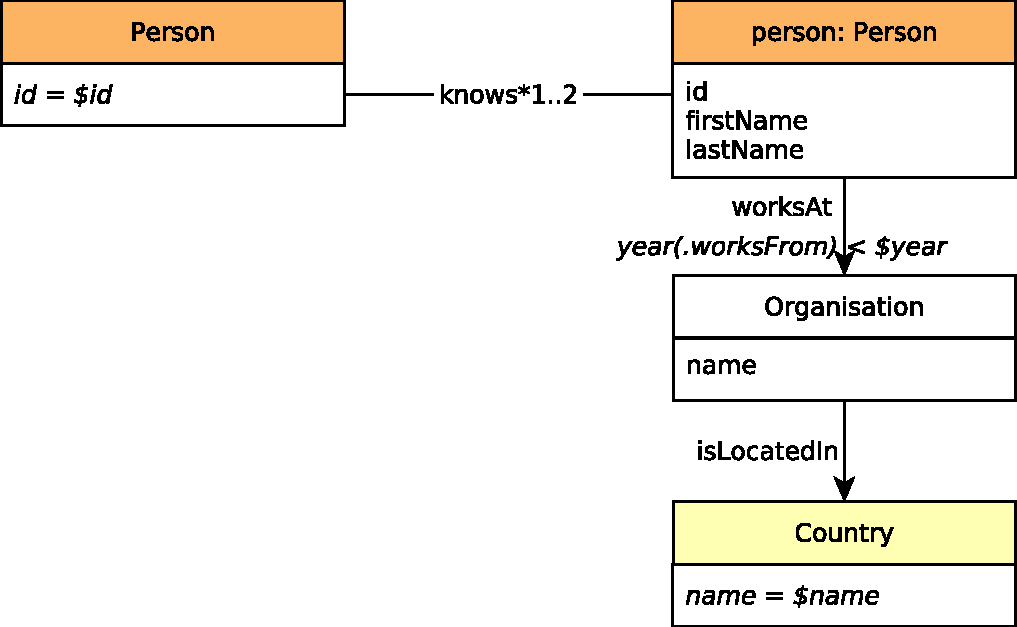
\includegraphics[scale=\patternscale,margin=0cm .2cm]{patterns/interactive-complex-read-11}} \\ \hline
%
	desc. & Given a start Person, find that Person's friends and friends of friends
(excluding start Person) who started Working in some Company in a given
Country, before a given date (year).
 \\ \hline
%
	
		params &
		\innerCardVSpace{\begin{tabularx}{\attributeCardWidth}{|>{\paramNumberCell}c|>{\varNameCell}M|>{\typeCell}m{\typeWidth}|Y|} \hline
		$\mathsf{1}$ & Person.id
 & ID
 & \texttt{Person}
 \\ \hline
		$\mathsf{2}$ & Country.name
 & String
 & \texttt{Country}
 \\ \hline
		$\mathsf{3}$ & year
 & 32-bit Integer
 & \texttt{Date0}
 \\ \hline
		\end{tabularx}}\innerCardVSpace \\ \hline
	
%
	
		result &
		\innerCardVSpace{\begin{tabularx}{\attributeCardWidth}{|>{\resultNumberCell}c|>{\varNameCell}M|>{\typeCell}m{\typeWidth}|>{\resultOriginCell}c|Y|} \hline
		$\mathsf{1}$ & Person.id & ID & R &
				\texttt{personId}
 \\ \hline
		$\mathsf{2}$ & Person.firstName & String & R &
				\texttt{personFirstName}
 \\ \hline
		$\mathsf{3}$ & Person.lastName & String & R &
				\texttt{personLastName}
 \\ \hline
		$\mathsf{4}$ & Person-worksAt-\textgreater{}Organisation.name & String & R &
				\texttt{organizationName}
 \\ \hline
		$\mathsf{5}$ & Person-worksAt-\textgreater{}.worksFrom & 32-bit Integer & R &
				\texttt{organizationWorkFromYear}
 \\ \hline
		\end{tabularx}}\innerCardVSpace \\ \hline
	
%
	
		sort		&
		\innerCardVSpace{\begin{tabularx}{\attributeCardWidth}{|>{\sortNumberCell}c|>{\varNameCell}M|>{\directionCell}c|Y|} \hline
		$\mathsf{1}$ & Person-worksAt-\textgreater{}.worksFrom
 & $\asc
$ &  \\ \hline
		$\mathsf{2}$ & Person.id
 & $\asc
$ &  \\ \hline
		$\mathsf{3}$ & Person-worksAt-\textgreater{}Organisation.name
 & $\desc
$ &  \\ \hline
		\end{tabularx}}\innerCardVSpace \\ \hline
	%
	limit & 10 \\ \hline
	%
	CPs &
	\multicolumn{1}{>{\raggedright}l|}{
		\chokePoint{1.3}, 
		\chokePoint{2.3}, 
		\chokePoint{2.4}, 
		\chokePoint{3.3}
		} \\ \hline
	%
	relevance &
		\footnotesize This query looks for paths of length two or three, starting from a Person, moving to friends or friends of friends,
and ending at a Company. In this query, there are selective joins and a top k order by that can be exploited for
optimizations.
 \\ \hline%
\end{tabularx}
\queryCardVSpace

% change \emph back to the old one
\let\emph\oldemph
\renewcommand*{\arraystretch}{1.1}

\subsection*{Interactive / complex / 12}
\label{section:interactive-complex-read-12}

% change \emph{} to use sans-serif font
\let\oldemph\emph
\renewcommand{\emph}[1]{{\footnotesize \sf #1}}

\renewcommand{\currentQueryCard}{12}
\marginpar{
	\raggedleft
	\vspace{0.22ex}

	\queryRefCard{interactive-complex-read-01}{Interactive}{1}\\
	\queryRefCard{interactive-complex-read-02}{Interactive}{2}\\
	\queryRefCard{interactive-complex-read-03}{Interactive}{3}\\
	\queryRefCard{interactive-complex-read-04}{Interactive}{4}\\
	\queryRefCard{interactive-complex-read-05}{Interactive}{5}\\
	\queryRefCard{interactive-complex-read-06}{Interactive}{6}\\
	\queryRefCard{interactive-complex-read-07}{Interactive}{7}\\
	\queryRefCard{interactive-complex-read-08}{Interactive}{8}\\
	\queryRefCard{interactive-complex-read-09}{Interactive}{9}\\
	\queryRefCard{interactive-complex-read-10}{Interactive}{10}\\
	\queryRefCard{interactive-complex-read-11}{Interactive}{11}\\
	\queryRefCard{interactive-complex-read-12}{Interactive}{12}\\
	\queryRefCard{interactive-complex-read-13}{Interactive}{13}\\
	\queryRefCard{interactive-complex-read-14}{Interactive}{14}\\
}

\noindent\begin{tabularx}{\queryCardWidth}{|>{\queryPropertyCell}p{\queryPropertyCellWidth}|X|}
	\hline
	query & Interactive / complex / 12 \\ \hline
%
	title & Expert search \\ \hline
%
	pattern & \hfill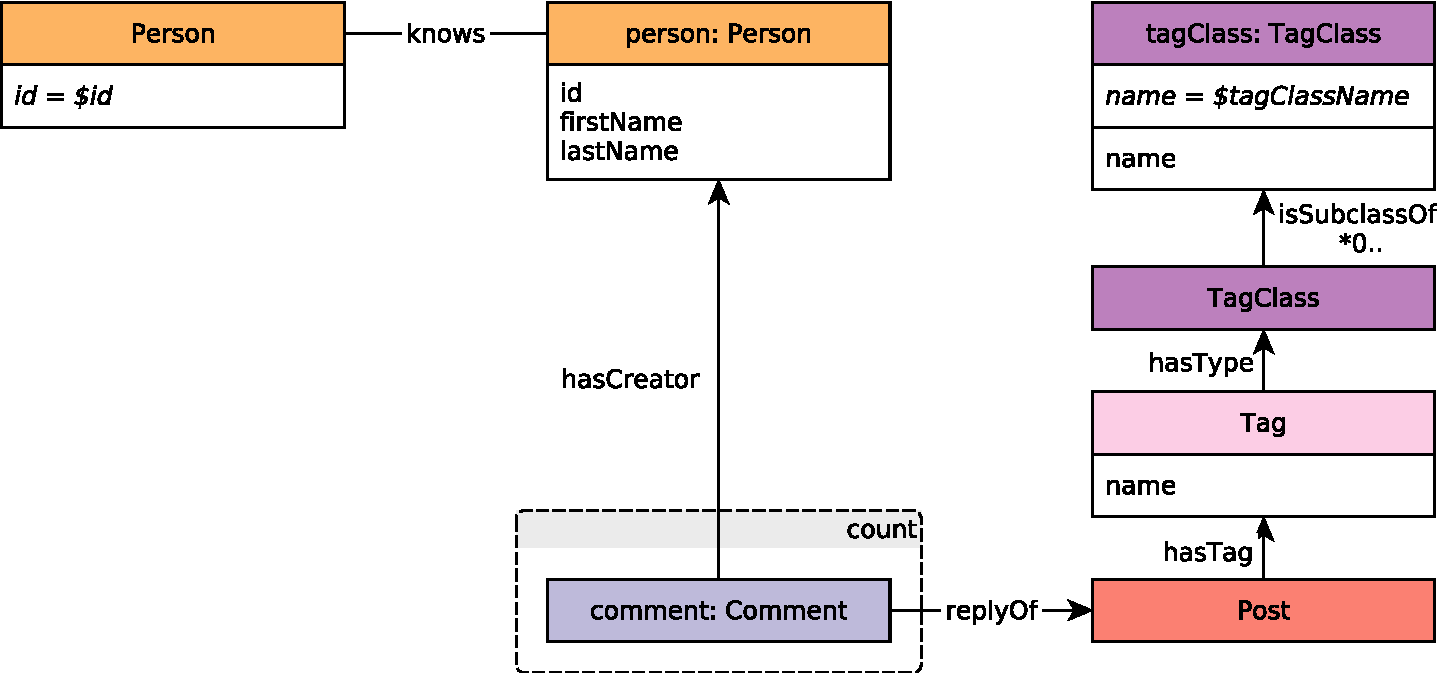
\includegraphics[scale=\patternscale,margin=0cm .2cm]{patterns/interactive-complex-read-12}\hfill \\ \hline
%
	desc. & Given a start Person, find the Comments that this Person's friends made
in reply to Posts, considering only those Comments that are immediate
(1-hop) replies to Posts, not the transitive (multi-hop) case. Only
consider Posts with a Tag in a given TagClass or in a descendent of that
TagClass. Count the number of these reply Comments, and collect the Tags
that were attached to the Posts they replied to, but only collect Tags
with the given TagClass or with a descendant of that TagClass Return
Persons with at least one reply, the reply count, and the collection of
Tags.
 \\ \hline
%
	
		params &
		\innerCardVSpace{\begin{tabularx}{\attributeCardWidth}{|>{\paramNumberCell}c|>{\varNameCell}M|>{\typeCell}m{\typeWidth}|Y|} \hline
		$\mathsf{1}$ & Person.id
 & ID
 &  \\ \hline
		$\mathsf{2}$ & TagClass.name
 & String
 &  \\ \hline
		\end{tabularx}}\innerCardVSpace \\ \hline
	
%
	
		result &
		\innerCardVSpace{\begin{tabularx}{\attributeCardWidth}{|>{\resultNumberCell}c|>{\varNameCell}M|>{\typeCell}m{\typeWidth}|>{\resultOriginCell}c|Y|} \hline
		$\mathsf{1}$ & Person.id & ID & R &
				 \\ \hline
		$\mathsf{2}$ & Person.firstName & String & R &
				 \\ \hline
		$\mathsf{3}$ & Person.lastName & String & R &
				 \\ \hline
		$\mathsf{4}$ & \{Tag.name\} & \{String\} & R &
				 \\ \hline
		$\mathsf{5}$ & count & 32-bit Integer & A &
				Number of reply Comments
 \\ \hline
		\end{tabularx}}\innerCardVSpace \\ \hline
	
%
	
		sort		&
		\innerCardVSpace{\begin{tabularx}{\attributeCardWidth}{|>{\sortNumberCell}c|>{\varNameCell}M|>{\directionCell}c|Y|} \hline
		$\mathsf{1}$ & count
 & $\desc
$ &  \\ \hline
		$\mathsf{2}$ & Person.id
 & $\asc
$ &  \\ \hline
		\end{tabularx}}\innerCardVSpace \\ \hline
	%
	limit & 20 \\ \hline
	%
	CPs &
	\multicolumn{1}{>{\raggedright}l|}{
		\chokePoint{1.5}, 
		\chokePoint{3.3}, 
		\chokePoint{7.2}, 
		\chokePoint{7.3}
		} \\ \hline
	%
	relevance &
		\small This query looks for paths of length three, starting at a Person, moving to its friends, the to their Comments and
ending at the Post the Comments are replying. The chain from original post to the reply is transitive. The traversal
may be initiated at either end, the system may note that this is a tree, hence leaf to root is always best. Additionally,
a hash table can be built from either end, e.g. from the friends of self, from the tags in the category, from the or
other.
 \\ \hline%
\end{tabularx}
\queryCardVSpace

% change \emph back to the old one
\renewcommand{\emph}[1]{\oldemph{#1}}
\renewcommand*{\arraystretch}{1.1}

\subsection*{Interactive / complex / 13}
\label{sec:interactive-complex-read-13}

\noindent\begin{tabularx}{\queryCardWidth}{|>{\queryPropertyCell}c|X|}
	\hline
	query & Interactive / complex / 13 \\ \hline
%
	title & Single shortest path \\ \hline
%
    pattern & \hfill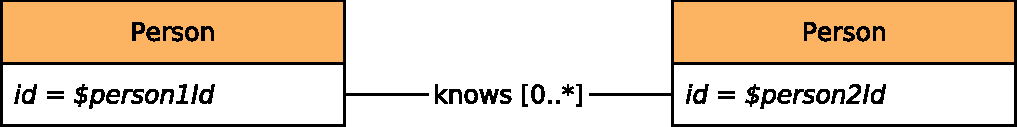
\includegraphics[scale=\patternscale,margin=0cm .2cm]{patterns/interactive-complex-read-13}\hfill\vadjust{} \\ \hline
%
	desc. & Given two Persons, find the shortest path between these two Persons in
the subgraph induced by the Knows relationships.

Return the length of this path:

\begin{itemize}
\tightlist
\item
  \(-1\) : no path found
\item
  \(0\): start person = end person
\item
  \(> 0\): regular case
\end{itemize}
 \\ \hline
%
	
%
    
        params &
        \innerCardVSpace{\begin{tabularx}{\attributeCardWidth}{|>{\paramNumberCell}c|>{\varNameCell}M|>{\typeCell}m{\typeWidth}|Y|} \hline
        \cellcolor{parameter} \color{white} \footnotesize $\mathsf{1}$ &person1.id& ID &  \\ \hline
        \cellcolor{parameter} \color{white} \footnotesize $\mathsf{2}$ &person2.id& ID &  \\ \hline
        \end{tabularx}}\innerCardVSpace \\ \hline
	
%
	
        result &
        \innerCardVSpace{\begin{tabularx}{\attributeCardWidth}{|>{\resultNumberCell}c|>{\varNameCell}M|>{\typeCell}m{\typeWidth}|>{\resultOriginCell}c|Y|} \hline
        $\mathsf{1}$ & length & 32-bit Integer &C&
                 \\ \hline
        \end{tabularx}}\innerCardVSpace \\ \hline
	
%
	%
	%
	CPs &
	\multicolumn{1}{>{\raggedright}l|}{
	    \chokePoint{3.3}, 
	    \chokePoint{7.2}, 
	    \chokePoint{7.3}
	    } \\ \hline
	%
    relevance &
        \small This query looks for a variable length path, starting at a given Person and finishing at an another given Person.
Proper cardinality estimation and search space prunning, will be crucial. This query also allows for possible parallel
implementations.
 \\ \hline%
\end{tabularx}
\queryCardVSpace
\renewcommand*{\arraystretch}{1.1}

\subsection*{Interactive / complex / 14}
\label{sec:interactive-complex-read-14}

\noindent\begin{tabularx}{\queryCardWidth}{|>{\queryPropertyCell}p{\queryPropertyCellWidth}|X|}
	\hline
	query & Interactive / complex / 14 \\ \hline
%
	title & Weighted/unweighted paths
 \\ \hline
%
	pattern & \hfill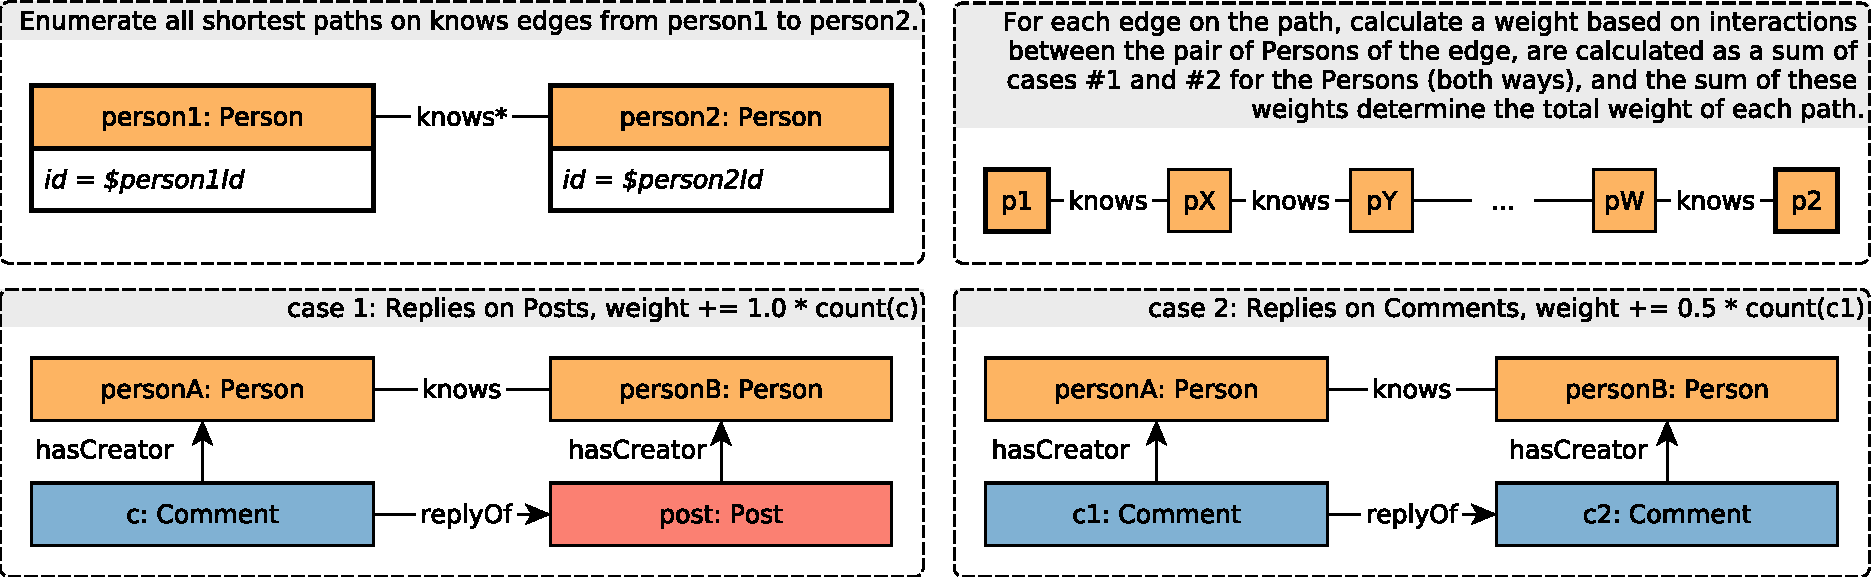
\includegraphics[scale=\patternscale,margin=0cm .2cm]{patterns/interactive-complex-read-14}\hfill\vadjust{} \\ \hline
%
	desc. & Given two Persons, find all (unweighted) shortest paths between these
two Persons, in the subgraph induced by the Knows relationship. Then,
for each path calculate a weight. The nodes in the path are Persons, and
the weight of a path is the sum of weights between every pair of
consecutive Person nodes in the path. The weight for a pair of Persons
is calculated such that every reply (by one of the Persons) to a Post
(by the other Person) contributes 1.0, and every reply (by ones of the
Persons) to a Comment (by the other Person) contributes 0.5. Return all
the paths with shortest length, and their weights. Do not return any
rows if there is now path between the two Persons.
 \\ \hline
%
	
%
	
		params &
		\innerCardVSpace{\begin{tabularx}{\attributeCardWidth}{|>{\paramNumberCell}c|>{\varNameCell}M|>{\typeCell}m{\typeWidth}|Y|} \hline
		$\mathsf{1}$ & person1.id
 & ID
 &  \\ \hline
		$\mathsf{2}$ & person2.id
 & ID
 &  \\ \hline
		\end{tabularx}}\innerCardVSpace \\ \hline
	
%
	
		result &
		\innerCardVSpace{\begin{tabularx}{\attributeCardWidth}{|>{\resultNumberCell}c|>{\varNameCell}M|>{\typeCell}m{\typeWidth}|>{\resultOriginCell}c|Y|} \hline
		$\mathsf{1}$ & {[}Person.id{]}
 & {[}ID{]}
 & R &
				Identifiers representing an ordered sequence of the Persons in the path
 \\ \hline
		$\mathsf{2}$ & weight
 & 64-bit Float
 & R &
				 \\ \hline
		\end{tabularx}}\innerCardVSpace \\ \hline
	
%
	
		sort		&
		\innerCardVSpace{\begin{tabular}{|>{\sortNumberCell}c|>{\varNameCell}l|>{\directionCell}c|} \hline
		$\mathsf{1}$ & weight
 & $\desc
$ \\ \hline
		\end{tabular}}\innerCardVSpace \\ \hline
	%
	%
	CPs &
	\multicolumn{1}{>{\raggedright}l|}{
		\chokePoint{3.3}, 
		\chokePoint{7.2}, 
		\chokePoint{7.3}
		} \\ \hline
	%
	relevance &
		\small This query looks for a variable length path, starting at a given Person and finishing at an another given Person. This
is a more complex query as not only requires computing the path length, but returning it and computing a weight.
To compute this weight one must look for smaller sub-queries with paths of length three, formed by the two Persons
at each step, a Post and a Comment.
 \\ \hline%
\end{tabularx}
\queryCardVSpace

% reset counter to make sure the last query card isn't stuck in highlighted mode
\renewcommand{\currentQueryCard}{0}


\renewcommand*{\arraystretch}{1.1}

\noindent\begin{tabularx}{17cm}{|p{1.95cm}|X|}
	\hline
	number      & 1                                                          \\ \hline
%
	title       & Friends with certain name                                                           \\ \hline
	\multicolumn{2}{|c|}{ 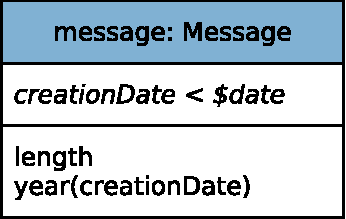
\includegraphics[scale=\patternscale,margin=0cm .2cm]{patterns/q01}} \\ \hline
	description & Given a start Person, find Persons with a given first name that the
start Person is connected to (excluding start Person) by at most 3 steps
via Knows relationships. Return Persons, including summaries of the
Persons workplaces and places of study.
 \\ \hline
	
%
	parameters  &
	\vspace{1.1ex}{\begin{tabularx}{14.2cm}{|c|l|m{2cm}|Y|} \hline
	\cellcolor{black!70} \color{white} $\mathsf{1}$ & \varname{Person.id} & \cellcolor{gray!20} \vartype{ID} &  \\\hline
	\cellcolor{black!70} \color{white} $\mathsf{2}$ & \varname{Person.firstName} & \cellcolor{gray!20} \vartype{String} &  \\
	\end{tabularx}} \\ \hline
%
	result      &
	\vspace{1.1ex}{\begin{tabularx}{14.2cm}{|c|l|m{2cm}|Y|} \hline
	\cellcolor{black!70} \color{white} $\mathsf{1}$ & \varname{Person.id} & \cellcolor{gray!20} \vartype{ID} &  \\\hline
	\cellcolor{black!70} \color{white} $\mathsf{2}$ & \varname{Person.lastName} & \cellcolor{gray!20} \vartype{String} &  \\\hline
	\cellcolor{black!70} \color{white} $\mathsf{3}$ & \varname{Person.birthday} & \cellcolor{gray!20} \vartype{Date} &  \\\hline
	\cellcolor{black!70} \color{white} $\mathsf{4}$ & \varname{Person.creationDate} & \cellcolor{gray!20} \vartype{DateTime} &  \\\hline
	\cellcolor{black!70} \color{white} $\mathsf{5}$ & \varname{Person.gender} & \cellcolor{gray!20} \vartype{String} &  \\\hline
	\cellcolor{black!70} \color{white} $\mathsf{6}$ & \varname{Person.browserUsed} & \cellcolor{gray!20} \vartype{String} &  \\\hline
	\cellcolor{black!70} \color{white} $\mathsf{7}$ & \varname{Person.locationIP} & \cellcolor{gray!20} \vartype{String} &  \\\hline
	\cellcolor{black!70} \color{white} $\mathsf{8}$ & \varname{\{Person.emails\}} & \cellcolor{gray!20} \vartype{\{String\}} &  \\\hline
	\cellcolor{black!70} \color{white} $\mathsf{9}$ & \varname{\{Person.language\}} & \cellcolor{gray!20} \vartype{\{String\}} &  \\\hline
	\cellcolor{black!70} \color{white} $\mathsf{10}$ & \varname{Person-isLocatedIn->Place.name} & \cellcolor{gray!20} \vartype{String} &  \\\hline
	\cellcolor{black!70} \color{white} $\mathsf{11}$ & \varname{\{Person-studyAt->University.name, Person-studyAt->.classYear, Person-studyAt->University-isLocatedIn->City.name\}} & \cellcolor{gray!20} \vartype{\{<String, 32-bit Integer, String>\}} &  \\\hline
	\cellcolor{black!70} \color{white} $\mathsf{12}$ & \varname{\{Person-workAt->Company.name, Person-workAt->.workFrom, Person-workAt->Company-isLocatedIn->Country.name\}} & \cellcolor{gray!20} \vartype{\{<String, 32-bit Integer, String>\}} &  \\
	\end{tabularx}} \\ \hline
	%
	sort        &
	\vspace{1.1ex}{\begin{tabular}{|c|l|c|} \hline
	\cellcolor{black!70} \color{white} $\mathsf{1}$ & \varname{distance from person} & \cellcolor{gray!20} $\asc$ \\\hline
	\cellcolor{black!70} \color{white} $\mathsf{2}$ & \varname{Person.lastName} & \cellcolor{gray!20} $\asc$ \\\hline
	\cellcolor{black!70} \color{white} $\mathsf{3}$ & \varname{Person.id} & \cellcolor{gray!20} $\asc$ \\
	\end{tabular}} \\ \hline
	%
	limit       & 20 \\ \hline
	%
	choke points &
	\multicolumn{1}{>{\raggedright}X|}{
		}\\ \hline
\end{tabularx}
\clearpage
\renewcommand*{\arraystretch}{1.1}

\noindent\begin{tabularx}{17cm}{|p{1.95cm}|X|}
	\hline
	workload    & Interactive \\ \hline
%
	query       & 2 \\ \hline
%
	title       & Recent posts and comments by your friends \\ \hline
%
    pattern     & \hfill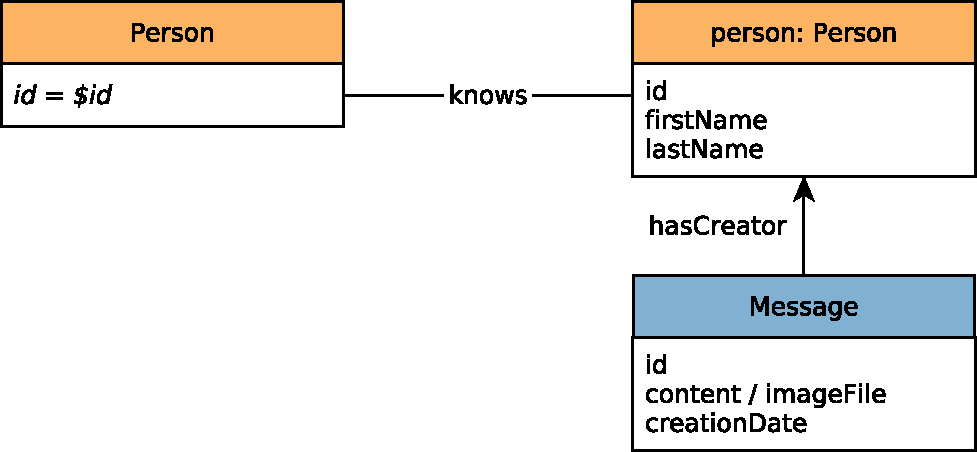
\includegraphics[scale=\patternscale,margin=0cm .2cm]{patterns/interactive02}\hfill\vadjust{} \\ \hline
%
	description & Given a start Person, find (most recent) Messages from all of that
Person's friends, that were created before (and including) a given date.
 \\ \hline
	
%
	parameters  &
	\vspace{1.1ex}{\begin{tabularx}{14.2cm}{|c|M|m{2cm}|Y|} \hline
	\cellcolor{black!70} \color{white} $\mathsf{1}$ & \varname{Person.id} & \cellcolor{gray!20} \vartype{ID} &  \\ \hline
	\cellcolor{black!70} \color{white} $\mathsf{2}$ & \varname{date} & \cellcolor{gray!20} \vartype{DateTime} &  \\ \hline
	\end{tabularx}}\vspace{1.1ex} \\ \hline
%
	result      &
	\vspace{1.1ex}{\begin{tabularx}{14.2cm}{|c|M|m{2cm}|Y|} \hline
	\cellcolor{black!70} \color{white} $\mathsf{1}$ & \varname{Message-hasCreator->Person.id} & \cellcolor{gray!20} \vartype{ID} &  \\ \hline
	\cellcolor{black!70} \color{white} $\mathsf{2}$ & \varname{Message-hasCreator->Person.firstName} & \cellcolor{gray!20} \vartype{String} &  \\ \hline
	\cellcolor{black!70} \color{white} $\mathsf{3}$ & \varname{Message-hasCreator->Person.lastName} & \cellcolor{gray!20} \vartype{String} &  \\ \hline
	\cellcolor{black!70} \color{white} $\mathsf{4}$ & \varname{Message.id} & \cellcolor{gray!20} \vartype{ID} &  \\ \hline
	\cellcolor{black!70} \color{white} $\mathsf{5}$ & \varname{Message.content or Post.imageFile} & \cellcolor{gray!20} \vartype{String} &  \\ \hline
	\cellcolor{black!70} \color{white} $\mathsf{6}$ & \varname{Message.creationDate} & \cellcolor{gray!20} \vartype{DateTime} &  \\ \hline
	\end{tabularx}}\vspace{1.1ex} \\ \hline
	%
	sort        &
	\vspace{1.1ex}{\begin{tabular}{|c|l|c|} \hline
	\cellcolor{black!70} \color{white} $\mathsf{1}$ & \varname{Message.creationDate} & \cellcolor{gray!20} $\desc$ \\ \hline
	\cellcolor{black!70} \color{white} $\mathsf{2}$ & \varname{Message.id} & \cellcolor{gray!20} $\asc$ \\ \hline
	\end{tabular}}\vspace{1.1ex} \\ \hline
	%
	limit       & 20 \\ \hline
	%
	choke points &
	\multicolumn{1}{>{\raggedright}X|}{
		}\\ \hline
\end{tabularx}
\clearpage
\renewcommand*{\arraystretch}{1.1}

\noindent\begin{tabularx}{17cm}{|p{1.95cm}|X|}
	\hline
	workload    & Interactive \\ \hline
%
	query       & 3 \\ \hline
%
	title       & Friends and friends of friends that have been to countries X and Y \\ \hline
%
    pattern     & \hfill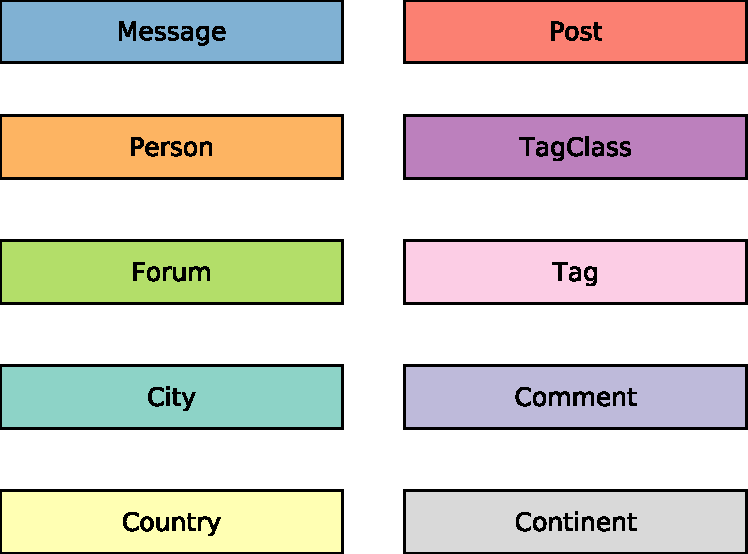
\includegraphics[scale=\patternscale,margin=0cm .2cm]{patterns/interactive03}\hfill\vadjust{} \\ \hline
%
	description & Given a start Person, find Persons that are their friends and friends of
friends (excluding start Person) that have made Posts/Comments in both
of the given Countries, X and Y, within a given period. Only Persons
that are foreign to Countries X and Y are considered, that is Persons
whose Location is not Country X or Country Y.
 \\ \hline
	
%
	parameters  &
	\vspace{1.1ex}{\begin{tabularx}{14.2cm}{|c|M|m{2cm}|Y|} \hline
	\cellcolor{black!70} \color{white} $\mathsf{1}$ & \varname{Person.id} & \cellcolor{gray!20} \vartype{ID} &  \\ \hline
	\cellcolor{black!70} \color{white} $\mathsf{2}$ & \varname{CountryX.name} & \cellcolor{gray!20} \vartype{String} &  \\ \hline
	\cellcolor{black!70} \color{white} $\mathsf{3}$ & \varname{CountryY.name} & \cellcolor{gray!20} \vartype{String} &  \\ \hline
	\cellcolor{black!70} \color{white} $\mathsf{4}$ & \varname{startDate} & \cellcolor{gray!20} \vartype{Date} & beginning of requested period \\ \hline
	\cellcolor{black!70} \color{white} $\mathsf{5}$ & \varname{duration} & \cellcolor{gray!20} \vartype{32-bit Integer} & duration of requested period, in days the interval [startDate, startDate + Duration) is closed-open \\ \hline
	\end{tabularx}}\vspace{1.1ex} \\ \hline
%
	result      &
	\vspace{1.1ex}{\begin{tabularx}{14.2cm}{|c|M|m{2cm}|Y|} \hline
	\cellcolor{black!70} \color{white} $\mathsf{1}$ & \varname{Person.id} & \cellcolor{gray!20} \vartype{ID} &  \\ \hline
	\cellcolor{black!70} \color{white} $\mathsf{2}$ & \varname{Person.firstName} & \cellcolor{gray!20} \vartype{String} &  \\ \hline
	\cellcolor{black!70} \color{white} $\mathsf{3}$ & \varname{Person.lastName} & \cellcolor{gray!20} \vartype{String} &  \\ \hline
	\cellcolor{black!70} \color{white} $\mathsf{4}$ & \varname{countX} & \cellcolor{gray!20} \vartype{32-bit Integer} & number of Messages from Country X made by Person within the given time \\ \hline
	\cellcolor{black!70} \color{white} $\mathsf{5}$ & \varname{countY} & \cellcolor{gray!20} \vartype{32-bit Integer} & number of Messages from Country Y made by Person within the given time \\ \hline
	\cellcolor{black!70} \color{white} $\mathsf{6}$ & \varname{count} & \cellcolor{gray!20} \vartype{32-bit Integer} & countX + countY \\ \hline
	\end{tabularx}}\vspace{1.1ex} \\ \hline
	%
	sort        &
	\vspace{1.1ex}{\begin{tabular}{|c|l|c|} \hline
	\cellcolor{black!70} \color{white} $\mathsf{1}$ & \varname{countX} & \cellcolor{gray!20} $\desc$ \\ \hline
	\cellcolor{black!70} \color{white} $\mathsf{2}$ & \varname{Person.id} & \cellcolor{gray!20} $\asc$ \\ \hline
	\end{tabular}}\vspace{1.1ex} \\ \hline
	%
	limit       & 20 \\ \hline
	%
	choke points &
	\multicolumn{1}{>{\raggedright}X|}{
		}\\ \hline
\end{tabularx}
\clearpage
\renewcommand*{\arraystretch}{1.1}

\noindent\begin{tabularx}{17cm}{|p{1.95cm}|X|}
	\hline
	workload    & Interactive \\ \hline
%
	query       & 4 \\ \hline
%
	title       & New topics \\ \hline
	\multicolumn{2}{|c|}{ 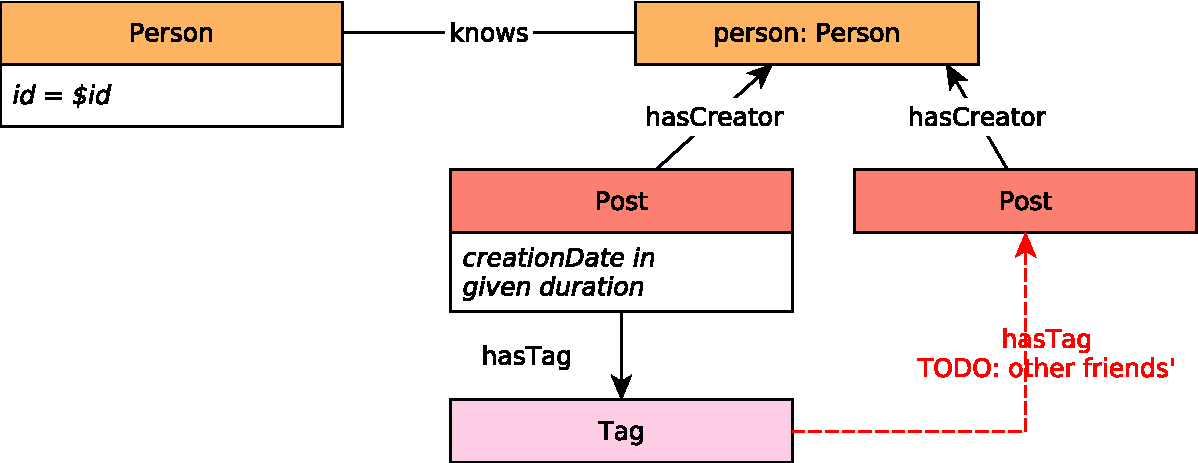
\includegraphics[scale=\patternscale,margin=0cm .2cm]{patterns/interactive04}} \\ \hline
	description & Given a start Person, find Tags that are attached to Posts that were
created by that Person's friends. Only include Tags that were attached
to friends' Posts created within a given time interval, and that were
never attached to friends' Posts created before this interval.
 \\ \hline
	
%
	parameters  &
	\vspace{1.1ex}{\begin{tabularx}{14.2cm}{|c|M|m{2cm}|Y|} \hline
	\cellcolor{black!70} \color{white} $\mathsf{1}$ & \varname{Person.id} & \cellcolor{gray!20} \vartype{ID} &  \\ \hline
	\cellcolor{black!70} \color{white} $\mathsf{2}$ & \varname{startDate} & \cellcolor{gray!20} \vartype{Date} &  \\ \hline
	\cellcolor{black!70} \color{white} $\mathsf{3}$ & \varname{duration} & \cellcolor{gray!20} \vartype{32-bit Integer} & duration of requested period, in days the interval [startDate, startDate + Duration) is closed-open \\ \hline
	\end{tabularx}}\vspace{1.1ex} \\ \hline
%
	result      &
	\vspace{1.1ex}{\begin{tabularx}{14.2cm}{|c|M|m{2cm}|Y|} \hline
	\cellcolor{black!70} \color{white} $\mathsf{1}$ & \varname{Tag.name} & \cellcolor{gray!20} \vartype{String} &  \\ \hline
	\cellcolor{black!70} \color{white} $\mathsf{2}$ & \varname{count} & \cellcolor{gray!20} \vartype{32-bit Integer} & number of Posts made within the given time interval that have this Tag \\ \hline
	\end{tabularx}}\vspace{1.1ex} \\ \hline
	%
	sort        &
	\vspace{1.1ex}{\begin{tabular}{|c|l|c|} \hline
	\cellcolor{black!70} \color{white} $\mathsf{1}$ & \varname{count} & \cellcolor{gray!20} $\desc$ \\ \hline
	\cellcolor{black!70} \color{white} $\mathsf{2}$ & \varname{Tag.name} & \cellcolor{gray!20} $\asc$ \\ \hline
	\end{tabular}}\vspace{1.1ex} \\ \hline
	%
	limit       & 10 \\ \hline
	%
	choke points &
	\multicolumn{1}{>{\raggedright}X|}{
		}\\ \hline
\end{tabularx}
\clearpage
\renewcommand*{\arraystretch}{1.1}

\noindent\begin{tabularx}{17cm}{|p{1.95cm}|X|}
	\hline
	workload    & Interactive \\ \hline
%
	query       & 5 \\ \hline
%
	title       & New groups \\ \hline
	\multicolumn{2}{|c|}{ 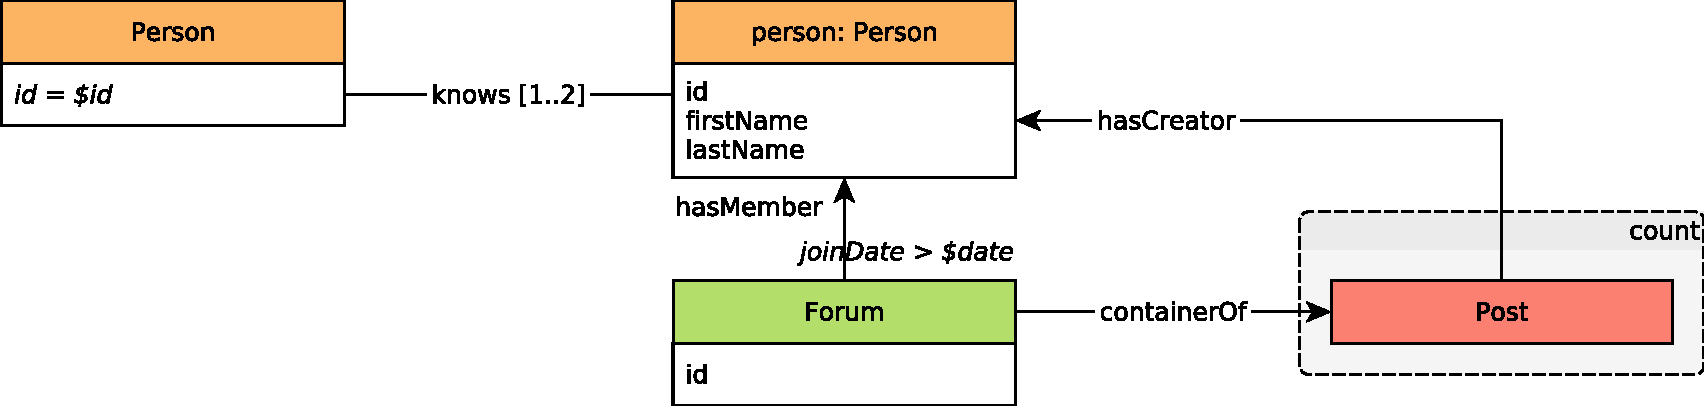
\includegraphics[scale=\patternscale,margin=0cm .2cm]{patterns/interactive05}} \\ \hline
	description & Given a start Person, find the Forums which that Person's friends and
friends of friends (excluding start Person) became Members of after a
given date. For each forum find the number of Posts that were created by
any of these Persons. For each Forum and consider only those Persons
which joined that particular Forum after the given date.
 \\ \hline
	
%
	parameters  &
	\vspace{1.1ex}{\begin{tabularx}{14.38cm}{|c|M|m{2cm}|Y} \hline
	\cellcolor{black!70} \color{white} $\mathsf{1}$ & \varname{Person.id} & \cellcolor{gray!20} \vartype{ID} &  \\\hline
	\cellcolor{black!70} \color{white} $\mathsf{2}$ & \varname{date} & \cellcolor{gray!20} \vartype{Date} &  \\
	\end{tabularx}} \\ \hline
%
	result      &
	\vspace{1.1ex}{\begin{tabularx}{14.38cm}{|c|M|m{2cm}|Y} \hline
	\cellcolor{black!70} \color{white} $\mathsf{1}$ & \varname{Forum.title} & \cellcolor{gray!20} \vartype{String} &  \\\hline
	\cellcolor{black!70} \color{white} $\mathsf{2}$ & \varname{count} & \cellcolor{gray!20} \vartype{32-bit Integer} & number of Posts made in Forum that were created by friends \\
	\end{tabularx}} \\ \hline
	%
	sort        &
	\vspace{1.1ex}{\begin{tabular}{|c|l|c|} \hline
	\cellcolor{black!70} \color{white} $\mathsf{1}$ & \varname{count} & \cellcolor{gray!20} $\desc$ \\\hline
	\cellcolor{black!70} \color{white} $\mathsf{2}$ & \varname{Forum.id} & \cellcolor{gray!20} $\asc$ \\
	\end{tabular}} \\ \hline
	%
	limit       & 20 \\ \hline
	%
	choke points &
	\multicolumn{1}{>{\raggedright}X|}{
		}\\ \hline
\end{tabularx}
\clearpage
\renewcommand*{\arraystretch}{1.1}

\noindent\begin{tabularx}{17cm}{|p{1.95cm}|X|}
	\hline
	workload    & interactive \\ \hline
%
	query       & 6 \\ \hline
%
	title       & Tag co-occurrence \\ \hline
	\multicolumn{2}{|c|}{ 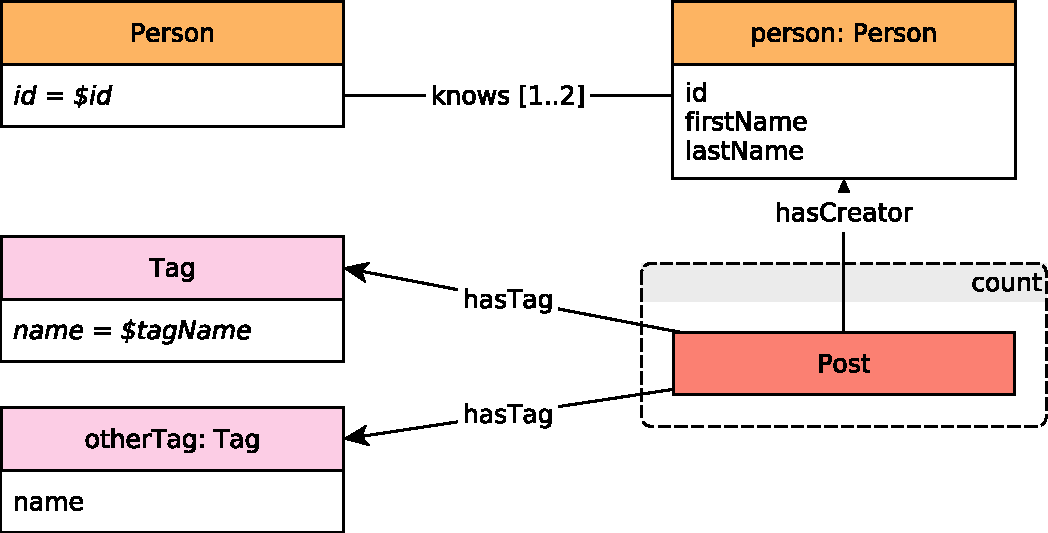
\includegraphics[scale=\patternscale,margin=0cm .2cm]{patterns/interactive06}} \\ \hline
	description & Given a start Person and some Tag, find the other Tags that occur
together with this Tag on Posts that were created by start Person's
friends and friends of friends (excluding start Person). Return For each
Tag, find the count of Posts that were created by these Persons, which
contain both this Tag and the given Tag.
 \\ \hline
	
%
	parameters  &
	\vspace{1.1ex}{\begin{tabularx}{14.38cm}{|c|M|m{2cm}|Y} \hline
	\cellcolor{black!70} \color{white} $\mathsf{1}$ & \varname{Person.id} & \cellcolor{gray!20} \vartype{ID} &  \\\hline
	\cellcolor{black!70} \color{white} $\mathsf{2}$ & \varname{Tag.name} & \cellcolor{gray!20} \vartype{String} &  \\
	\end{tabularx}} \\ \hline
%
	result      &
	\vspace{1.1ex}{\begin{tabularx}{14.38cm}{|c|M|m{2cm}|Y} \hline
	\cellcolor{black!70} \color{white} $\mathsf{1}$ & \varname{Tag.name} & \cellcolor{gray!20} \vartype{String} &  \\\hline
	\cellcolor{black!70} \color{white} $\mathsf{2}$ & \varname{count} & \cellcolor{gray!20} \vartype{32-bit Integer} & number of Posts that were created by friends and friends of friends, which contain this Tag \\
	\end{tabularx}} \\ \hline
	%
	sort        &
	\vspace{1.1ex}{\begin{tabular}{|c|l|c|} \hline
	\cellcolor{black!70} \color{white} $\mathsf{1}$ & \varname{count} & \cellcolor{gray!20} $\desc$ \\\hline
	\cellcolor{black!70} \color{white} $\mathsf{2}$ & \varname{Tag.name} & \cellcolor{gray!20} $\asc$ \\
	\end{tabular}} \\ \hline
	%
	limit       & 10 \\ \hline
	%
	choke points &
	\multicolumn{1}{>{\raggedright}X|}{
		}\\ \hline
\end{tabularx}
\clearpage
\renewcommand*{\arraystretch}{1.1}

\noindent\begin{tabularx}{17cm}{|p{1.95cm}|X|}
	\hline
	workload    & interactive \\ \hline
%
	query       & 7 \\ \hline
%
	title       & Recent likers \\ \hline
	\multicolumn{2}{|c|}{ 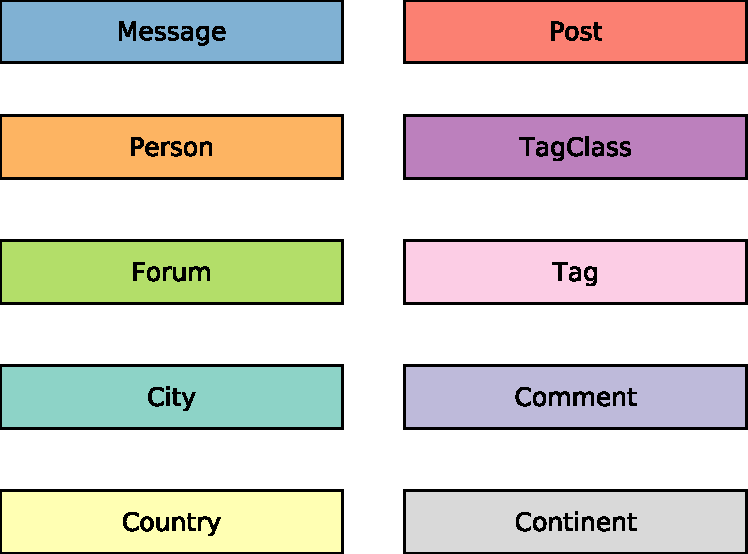
\includegraphics[scale=\patternscale,margin=0cm .2cm]{patterns/interactive07}} \\ \hline
	description & Given a start Person, find (most recent) Likes on any of start Person's
Messages. Find Persons that Liked any of start Person's Messages, the
Messages they liked most recently, creation date of that Like, and the
latency (in minutes) between creation of Messages and Like.
Additionally, for each Person found return a flag indicating whether the
liker is a friend of start Person. In the case that a Person Liked
multiple Messages at the same time, return the Message with lowest
identifier.
 \\ \hline
	
%
	parameters  &
	\vspace{1.1ex}{\begin{tabularx}{14.38cm}{|c|M|m{2cm}|Y} \hline
	\cellcolor{black!70} \color{white} $\mathsf{1}$ & \varname{Person.id} & \cellcolor{gray!20} \vartype{64-bit Integer} &  \\
	\end{tabularx}} \\ \hline
%
	result      &
	\vspace{1.1ex}{\begin{tabularx}{14.38cm}{|c|M|m{2cm}|Y} \hline
	\cellcolor{black!70} \color{white} $\mathsf{1}$ & \varname{Person.id} & \cellcolor{gray!20} \vartype{ID} &  \\\hline
	\cellcolor{black!70} \color{white} $\mathsf{2}$ & \varname{Person.firstName} & \cellcolor{gray!20} \vartype{String} &  \\\hline
	\cellcolor{black!70} \color{white} $\mathsf{3}$ & \varname{Person.lastName} & \cellcolor{gray!20} \vartype{String} &  \\\hline
	\cellcolor{black!70} \color{white} $\mathsf{4}$ & \varname{Like.creationDate} & \cellcolor{gray!20} \vartype{DateTime} &  \\\hline
	\cellcolor{black!70} \color{white} $\mathsf{5}$ & \varname{Message.id} & \cellcolor{gray!20} \vartype{ID} &  \\\hline
	\cellcolor{black!70} \color{white} $\mathsf{6}$ & \varname{Message.content or Post.imageFile} & \cellcolor{gray!20} \vartype{String} &  \\\hline
	\cellcolor{black!70} \color{white} $\mathsf{7}$ & \varname{latency} & \cellcolor{gray!20} \vartype{32-bit Integer} & duration between creation of\par Message and Like, in minutes \\\hline
	\cellcolor{black!70} \color{white} $\mathsf{8}$ & \varname{isNew} & \cellcolor{gray!20} \vartype{Boolean} & false if liker Person is friend of\par start Person, true otherwise \\
	\end{tabularx}} \\ \hline
	%
	sort        &
	\vspace{1.1ex}{\begin{tabular}{|c|l|c|} \hline
	\cellcolor{black!70} \color{white} $\mathsf{1}$ & \varname{Like.creationDate} & \cellcolor{gray!20} $\desc$ \\\hline
	\cellcolor{black!70} \color{white} $\mathsf{2}$ & \varname{Person.id} & \cellcolor{gray!20} $\asc$ \\
	\end{tabular}} \\ \hline
	%
	limit       & 20 \\ \hline
	%
	choke points &
	\multicolumn{1}{>{\raggedright}X|}{
		}\\ \hline
\end{tabularx}
\clearpage
\renewcommand*{\arraystretch}{1.1}

\noindent\begin{tabularx}{17cm}{|p{1.95cm}|X|}
	\hline
	workload    & Interactive \\ \hline
%
	query       & 8 \\ \hline
%
	title       & Recent replies \\ \hline
	\multicolumn{2}{|c|}{ 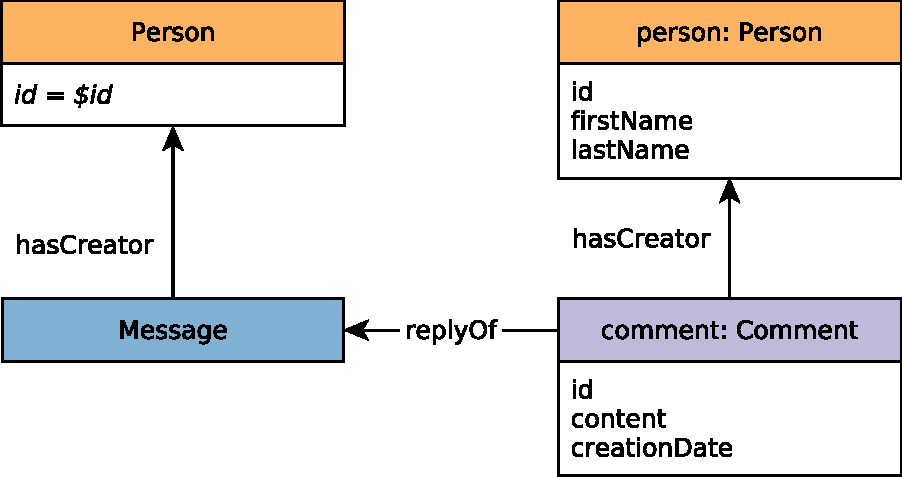
\includegraphics[scale=\patternscale,margin=0cm .2cm]{patterns/interactive08}} \\ \hline
	description & Given a start Person, find (most recent) Comments that are replies to
Messages of the start Person. Only consider immediate (1-hop) replies,
not the transitive (multi-hop) case. Return the reply Comments, and the
Person that created each reply Comment.
 \\ \hline
	
%
	parameters  &
	\vspace{1.1ex}{\begin{tabularx}{14.2cm}{|c|M|m{2cm}|Y|} \hline
	\cellcolor{black!70} \color{white} $\mathsf{1}$ & \varname{Person.id} & \cellcolor{gray!20} \vartype{ID} &  \\ \hline
	\end{tabularx}}\vspace{1.1ex} \\ \hline
%
	result      &
	\vspace{1.1ex}{\begin{tabularx}{14.2cm}{|c|M|m{2cm}|Y|} \hline
	\cellcolor{black!70} \color{white} $\mathsf{1}$ & \varname{Person.id} & \cellcolor{gray!20} \vartype{ID} &  \\ \hline
	\cellcolor{black!70} \color{white} $\mathsf{2}$ & \varname{Person.firstName} & \cellcolor{gray!20} \vartype{String} &  \\ \hline
	\cellcolor{black!70} \color{white} $\mathsf{3}$ & \varname{Person.lastName} & \cellcolor{gray!20} \vartype{String} &  \\ \hline
	\cellcolor{black!70} \color{white} $\mathsf{4}$ & \varname{Comment.creationDate} & \cellcolor{gray!20} \vartype{DateTime} &  \\ \hline
	\cellcolor{black!70} \color{white} $\mathsf{5}$ & \varname{Comment.id} & \cellcolor{gray!20} \vartype{ID} &  \\ \hline
	\cellcolor{black!70} \color{white} $\mathsf{6}$ & \varname{Comment.content} & \cellcolor{gray!20} \vartype{String} &  \\ \hline
	\end{tabularx}}\vspace{1.1ex} \\ \hline
	%
	sort        &
	\vspace{1.1ex}{\begin{tabular}{|c|l|c|} \hline
	\cellcolor{black!70} \color{white} $\mathsf{1}$ & \varname{Comment.creationDate} & \cellcolor{gray!20} $\desc$ \\ \hline
	\cellcolor{black!70} \color{white} $\mathsf{2}$ & \varname{Comment.id} & \cellcolor{gray!20} $\asc$ \\ \hline
	\end{tabular}}\vspace{1.1ex} \\ \hline
	%
	limit       & 20 \\ \hline
	%
	choke points &
	\multicolumn{1}{>{\raggedright}X|}{
		}\\ \hline
\end{tabularx}
\clearpage
\renewcommand*{\arraystretch}{1.1}

\noindent\begin{tabularx}{17cm}{|p{1.95cm}|X|}
	\hline
	workload    & Interactive \\ \hline
%
	query       & 9 \\ \hline
%
	title       & Recent posts and comments by friends or friends of friends \\ \hline
%
    pattern     & \hfill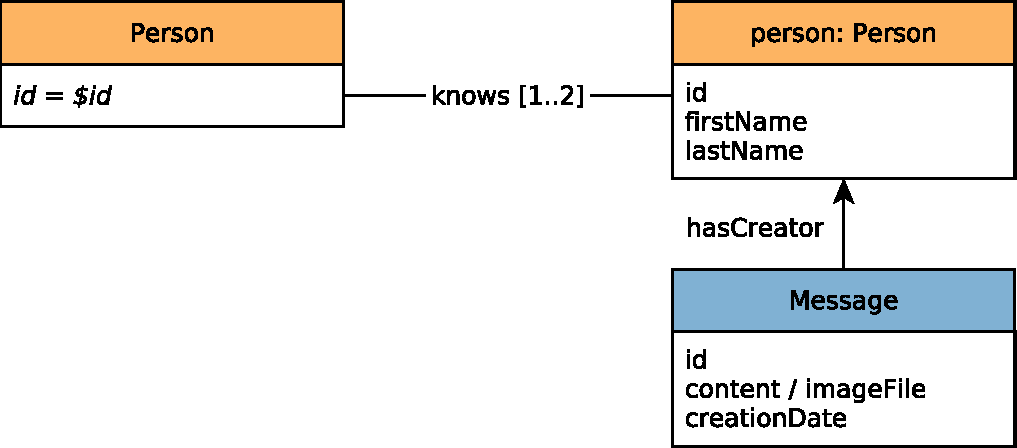
\includegraphics[scale=\patternscale,margin=0cm .2cm]{patterns/interactive09}\hfill\vadjust{} \\ \hline
%
	description & Given a start Person, find the (most recent) Messages created by that
Person's friends or friends of friends (excluding start Person). Only
consider the Messages created before a given date (excluding that date).
 \\ \hline
	
%
	parameters  &
	\vspace{1.1ex}{\begin{tabularx}{14.2cm}{|c|M|m{2cm}|Y|} \hline
	\cellcolor{black!70} \color{white} $\mathsf{1}$ & \varname{Person.id} & \cellcolor{gray!20} \vartype{ID} &  \\ \hline
	\cellcolor{black!70} \color{white} $\mathsf{2}$ & \varname{date} & \cellcolor{gray!20} \vartype{Date} &  \\ \hline
	\end{tabularx}}\vspace{1.1ex} \\ \hline
%
	result      &
	\vspace{1.1ex}{\begin{tabularx}{14.2cm}{|c|M|m{2cm}|Y|} \hline
	\cellcolor{black!70} \color{white} $\mathsf{1}$ & \varname{Message-hasCreator->Person.id} & \cellcolor{gray!20} \vartype{ID} &  \\ \hline
	\cellcolor{black!70} \color{white} $\mathsf{2}$ & \varname{Message-hasCreator->Person.firstName} & \cellcolor{gray!20} \vartype{String} &  \\ \hline
	\cellcolor{black!70} \color{white} $\mathsf{3}$ & \varname{Message-hasCreator->Person.lastName} & \cellcolor{gray!20} \vartype{String} &  \\ \hline
	\cellcolor{black!70} \color{white} $\mathsf{4}$ & \varname{Message.id} & \cellcolor{gray!20} \vartype{ID} &  \\ \hline
	\cellcolor{black!70} \color{white} $\mathsf{5}$ & \varname{Message.content or Post.imageFile} & \cellcolor{gray!20} \vartype{String} &  \\ \hline
	\cellcolor{black!70} \color{white} $\mathsf{6}$ & \varname{Message.creationDate} & \cellcolor{gray!20} \vartype{DateTime} &  \\ \hline
	\end{tabularx}}\vspace{1.1ex} \\ \hline
	%
	sort        &
	\vspace{1.1ex}{\begin{tabular}{|c|l|c|} \hline
	\cellcolor{black!70} \color{white} $\mathsf{1}$ & \varname{Message.creationDate} & \cellcolor{gray!20} $\desc$ \\ \hline
	\cellcolor{black!70} \color{white} $\mathsf{2}$ & \varname{Message.id} & \cellcolor{gray!20} $\asc$ \\ \hline
	\end{tabular}}\vspace{1.1ex} \\ \hline
	%
	limit       & 20 \\ \hline
	%
	choke points &
	\multicolumn{1}{>{\raggedright}X|}{
		}\\ \hline
\end{tabularx}
\clearpage
\renewcommand*{\arraystretch}{1.1}

\noindent\begin{tabularx}{17cm}{|p{1.95cm}|X|}
	\hline
	workload    & Interactive \\ \hline
%
	query       & 10 \\ \hline
%
	title       & Friend recommendation \\ \hline
%
    pattern     & \hfill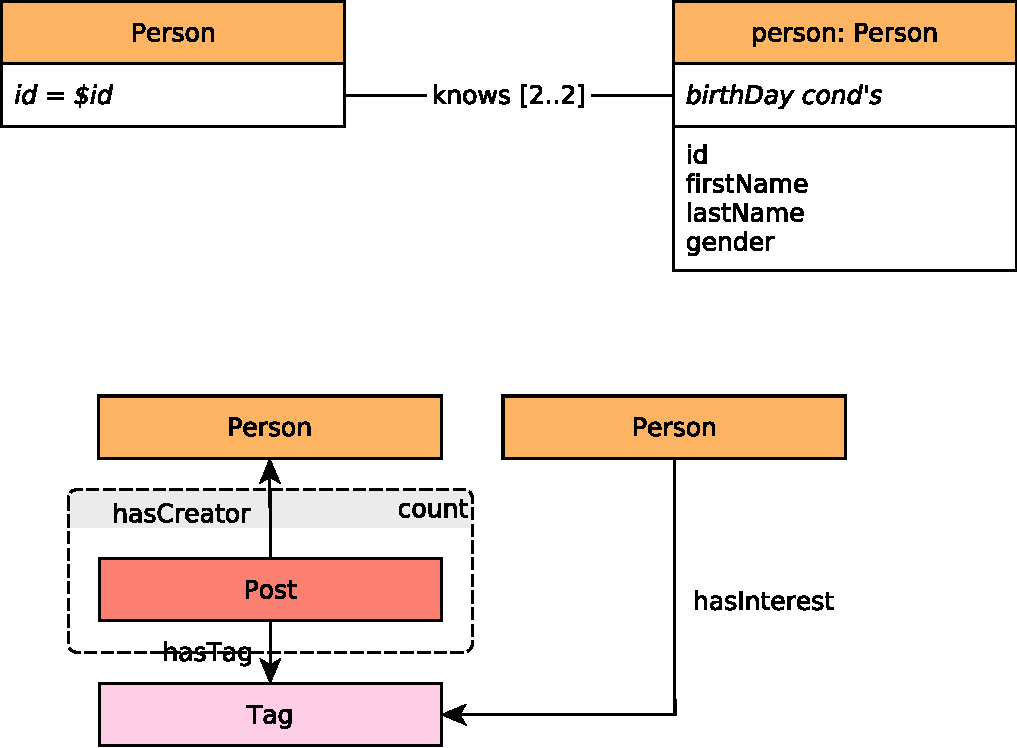
\includegraphics[scale=\patternscale,margin=0cm .2cm]{patterns/interactive10}\hfill\vadjust{} \\ \hline
%
	description & Given a start Person, find that Person's friends of friends (excluding
start Person, and immediate friends), who were born on or after the 21st
of a given month (in any year) and before the 22nd of the following
month. Calculate the similarity between each of these Persons and start
Person, where similarity for any Person is defined as follows:

\begin{itemize}
\tightlist
\item
  common = number of Posts created by that Person, such that the Post
  has a Tag that start Person is Interested in
\item
  uncommon = number of Posts created by that Person, such that the Post
  has no Tag that start Person is Interested in
\item
  similarity = common - uncommon
\end{itemize}
 \\ \hline
	
%
	parameters  &
	\vspace{1.1ex}{\begin{tabularx}{14.2cm}{|c|M|m{2cm}|Y|} \hline
	\cellcolor{black!70} \color{white} $\mathsf{1}$ & \varname{Person.id} & \cellcolor{gray!20} \vartype{ID} &  \\ \hline
	\cellcolor{black!70} \color{white} $\mathsf{2}$ & \varname{month} & \cellcolor{gray!20} \vartype{32-bit Integer} & between 1-12 \\ \hline
	\end{tabularx}}\vspace{1.1ex} \\ \hline
%
	result      &
	\vspace{1.1ex}{\begin{tabularx}{14.2cm}{|c|M|m{2cm}|Y|} \hline
	\cellcolor{black!70} \color{white} $\mathsf{1}$ & \varname{Person.id} & \cellcolor{gray!20} \vartype{ID} &  \\ \hline
	\cellcolor{black!70} \color{white} $\mathsf{2}$ & \varname{Person.firstName} & \cellcolor{gray!20} \vartype{String} &  \\ \hline
	\cellcolor{black!70} \color{white} $\mathsf{3}$ & \varname{Person.lastName} & \cellcolor{gray!20} \vartype{String} &  \\ \hline
	\cellcolor{black!70} \color{white} $\mathsf{4}$ & \varname{similarity} & \cellcolor{gray!20} \vartype{32-bit Integer} &  \\ \hline
	\cellcolor{black!70} \color{white} $\mathsf{5}$ & \varname{Person.gender} & \cellcolor{gray!20} \vartype{String} &  \\ \hline
	\cellcolor{black!70} \color{white} $\mathsf{6}$ & \varname{Person-isLocatedIn->Place.name} & \cellcolor{gray!20} \vartype{String} &  \\ \hline
	\end{tabularx}}\vspace{1.1ex} \\ \hline
	%
	sort        &
	\vspace{1.1ex}{\begin{tabular}{|c|l|c|} \hline
	\cellcolor{black!70} \color{white} $\mathsf{1}$ & \varname{similarity} & \cellcolor{gray!20} $\desc$ \\ \hline
	\cellcolor{black!70} \color{white} $\mathsf{2}$ & \varname{Person.id} & \cellcolor{gray!20} $\asc$ \\ \hline
	\end{tabular}}\vspace{1.1ex} \\ \hline
	%
	limit       & 10 \\ \hline
	%
	choke points &
	\multicolumn{1}{>{\raggedright}X|}{
		}\\ \hline
\end{tabularx}
\clearpage
\renewcommand*{\arraystretch}{1.1}

\noindent\begin{tabularx}{17cm}{|p{1.95cm}|X|}
	\hline
	workload    & interactive \\ \hline
%
	query       & 11 \\ \hline
%
	title       & Job referral \\ \hline
	\multicolumn{2}{|c|}{ 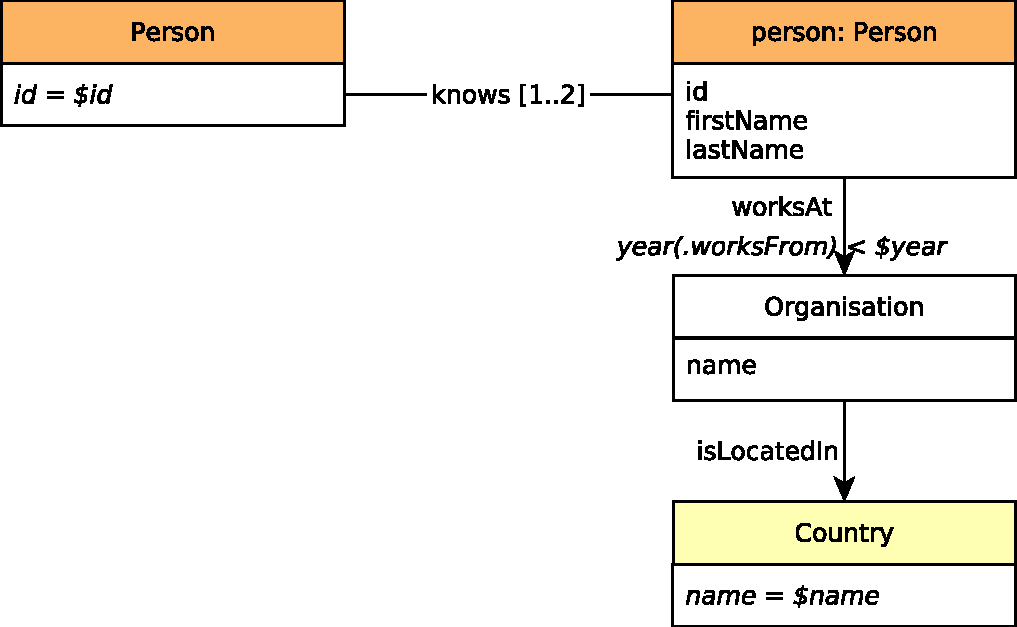
\includegraphics[scale=\patternscale,margin=0cm .2cm]{patterns/interactive11}} \\ \hline
	description & Given a start Person, find that Person's friends and friends of friends
(excluding start Person) who started Working in some Company in a given
Country, before a given date (year).
 \\ \hline
	
%
	parameters  &
	\vspace{1.1ex}{\begin{tabularx}{14.38cm}{|c|M|m{2cm}|Y} \hline
	\cellcolor{black!70} \color{white} $\mathsf{1}$ & \varname{Person.id} & \cellcolor{gray!20} \vartype{ID} &  \\\hline
	\cellcolor{black!70} \color{white} $\mathsf{2}$ & \varname{Country.name} & \cellcolor{gray!20} \vartype{String} &  \\\hline
	\cellcolor{black!70} \color{white} $\mathsf{3}$ & \varname{year} & \cellcolor{gray!20} \vartype{32-bit Integer} &  \\
	\end{tabularx}} \\ \hline
%
	result      &
	\vspace{1.1ex}{\begin{tabularx}{14.38cm}{|c|M|m{2cm}|Y} \hline
	\cellcolor{black!70} \color{white} $\mathsf{1}$ & \varname{Person.id} & \cellcolor{gray!20} \vartype{ID} &  \\\hline
	\cellcolor{black!70} \color{white} $\mathsf{2}$ & \varname{Person.firstName} & \cellcolor{gray!20} \vartype{String} &  \\\hline
	\cellcolor{black!70} \color{white} $\mathsf{3}$ & \varname{Person.lastName} & \cellcolor{gray!20} \vartype{String} &  \\\hline
	\cellcolor{black!70} \color{white} $\mathsf{4}$ & \varname{Person-worksAt->Organization.name} & \cellcolor{gray!20} \vartype{String} &  \\\hline
	\cellcolor{black!70} \color{white} $\mathsf{5}$ & \varname{Person-worksAt->.worksFrom} & \cellcolor{gray!20} \vartype{32-bit Integer} &  \\
	\end{tabularx}} \\ \hline
	%
	sort        &
	\vspace{1.1ex}{\begin{tabular}{|c|l|c|} \hline
	\cellcolor{black!70} \color{white} $\mathsf{1}$ & \varname{Person-worksAt->.worksFrom} & \cellcolor{gray!20} $\asc$ \\\hline
	\cellcolor{black!70} \color{white} $\mathsf{2}$ & \varname{Person.id} & \cellcolor{gray!20} $\asc$ \\\hline
	\cellcolor{black!70} \color{white} $\mathsf{3}$ & \varname{Person-worksAt->Organization.name} & \cellcolor{gray!20} $\desc$ \\
	\end{tabular}} \\ \hline
	%
	limit       & 10 \\ \hline
	%
	choke points &
	\multicolumn{1}{>{\raggedright}X|}{
		}\\ \hline
\end{tabularx}
\clearpage
\renewcommand*{\arraystretch}{1.1}

\noindent\begin{tabularx}{17cm}{|p{1.95cm}|X|}
	\hline
	workload    & interactive \\ \hline
%
	query       & 12 \\ \hline
%
	title       & Expert search \\ \hline
	\multicolumn{2}{|c|}{ 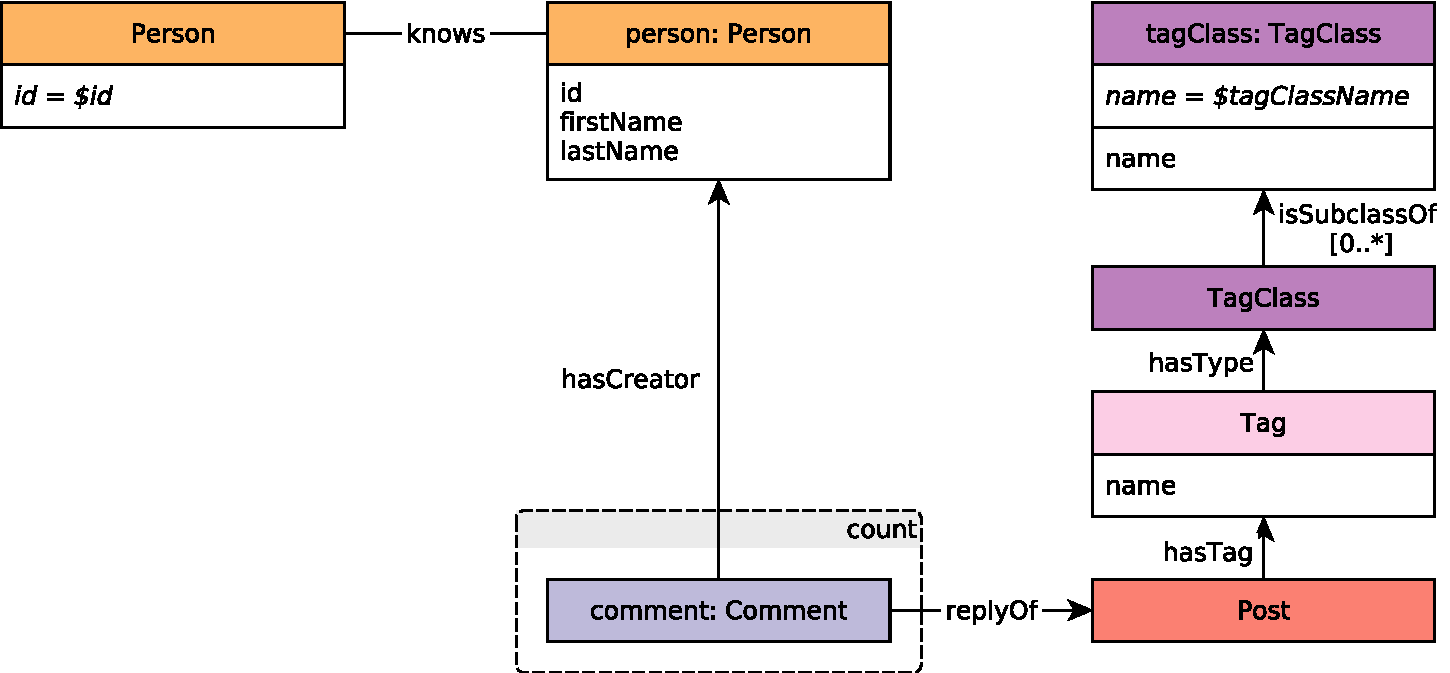
\includegraphics[scale=\patternscale,margin=0cm .2cm]{patterns/interactive12}} \\ \hline
	description & Given a start Person, find the Comments that this Person's friends made
in reply to Posts, considering only those Comments that are immediate
(1-hop) replies to Posts, not the transitive (multi-hop) case. Only
consider Posts with a Tag in a given TagClass or in a descendent of that
TagClass. Count the number of these reply Comments, and collect the Tags
(with valid tag class) that were attached to the Posts they replied to.
Return Persons with at least one reply, the reply count, and the
collection of Tags.
 \\ \hline
	
%
	parameters  &
	\vspace{1.1ex}{\begin{tabularx}{14.38cm}{|c|M|m{2cm}|Y} \hline
	\cellcolor{black!70} \color{white} $\mathsf{1}$ & \varname{Person.id} & \cellcolor{gray!20} \vartype{ID} &  \\\hline
	\cellcolor{black!70} \color{white} $\mathsf{2}$ & \varname{TagClass.name} & \cellcolor{gray!20} \vartype{String} &  \\
	\end{tabularx}} \\ \hline
%
	result      &
	\vspace{1.1ex}{\begin{tabularx}{14.38cm}{|c|M|m{2cm}|Y} \hline
	\cellcolor{black!70} \color{white} $\mathsf{1}$ & \varname{Person.id} & \cellcolor{gray!20} \vartype{ID} &  \\\hline
	\cellcolor{black!70} \color{white} $\mathsf{2}$ & \varname{Person.firstName} & \cellcolor{gray!20} \vartype{String} &  \\\hline
	\cellcolor{black!70} \color{white} $\mathsf{3}$ & \varname{Person.lastName} & \cellcolor{gray!20} \vartype{String} &  \\\hline
	\cellcolor{black!70} \color{white} $\mathsf{4}$ & \varname{\{Tag.name\}} & \cellcolor{gray!20} \vartype{\{String\}} &  \\\hline
	\cellcolor{black!70} \color{white} $\mathsf{5}$ & \varname{count} & \cellcolor{gray!20} \vartype{32-bit Integer} & number of reply Comments \\
	\end{tabularx}} \\ \hline
	%
	sort        &
	\vspace{1.1ex}{\begin{tabular}{|c|l|c|} \hline
	\cellcolor{black!70} \color{white} $\mathsf{1}$ & \varname{count} & \cellcolor{gray!20} $\desc$ \\\hline
	\cellcolor{black!70} \color{white} $\mathsf{2}$ & \varname{Person.id} & \cellcolor{gray!20} $\asc$ \\
	\end{tabular}} \\ \hline
	%
	limit       & 20 \\ \hline
	%
	choke points &
	\multicolumn{1}{>{\raggedright}X|}{
		}\\ \hline
\end{tabularx}
\clearpage
\renewcommand*{\arraystretch}{1.1}

\noindent\begin{tabularx}{17cm}{|p{1.95cm}|X|}
	\hline
	workload    & Interactive \\ \hline
%
	query       & 13 \\ \hline
%
	title       & Single shortest path \\ \hline
	\multicolumn{2}{|c|}{ 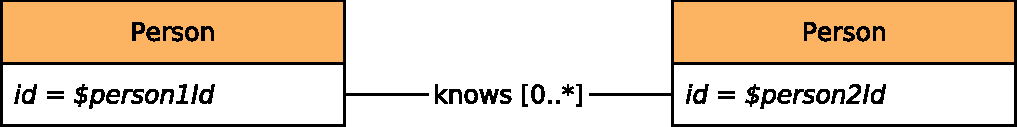
\includegraphics[scale=\patternscale,margin=0cm .2cm]{patterns/interactive13}} \\ \hline
	description & Given two Persons, find the shortest path between these two Persons in
the subgraph induced by the Knows relationships.

Return the length of this path:

\begin{itemize}
\tightlist
\item
  -1 : no path found
\item
  0: start person = end person
\item
  \textgreater{} 0: regular case
\end{itemize}
 \\ \hline
	
%
	parameters  &
	\vspace{1.1ex}{\begin{tabularx}{14.2cm}{|c|M|m{2cm}|Y|} \hline
	\cellcolor{black!70} \color{white} $\mathsf{1}$ & \varname{person1.id} & \cellcolor{gray!20} \vartype{ID} &  \\ \hline
	\cellcolor{black!70} \color{white} $\mathsf{2}$ & \varname{person2.id} & \cellcolor{gray!20} \vartype{ID} &  \\ \hline
	\end{tabularx}}\vspace{1.1ex} \\ \hline
%
	result      &
	\vspace{1.1ex}{\begin{tabularx}{14.2cm}{|c|M|m{2cm}|Y|} \hline
	\cellcolor{black!70} \color{white} $\mathsf{1}$ & \varname{length} & \cellcolor{gray!20} \vartype{32-bit Integer} &  \\ \hline
	\end{tabularx}}\vspace{1.1ex} \\ \hline
	%
	%
	choke points &
	\multicolumn{1}{>{\raggedright}X|}{
		}\\ \hline
\end{tabularx}
\clearpage
\renewcommand*{\arraystretch}{1.1}

\noindent\begin{tabularx}{17cm}{|p{1.95cm}|X|}
	\hline
	workload    & Interactive \\ \hline
%
	query       & 14 \\ \hline
%
	title       & Weighted/unweighted paths \\ \hline
	\multicolumn{2}{|c|}{ 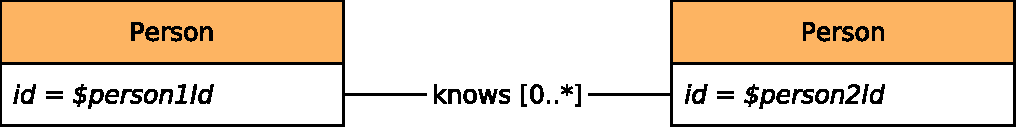
\includegraphics[scale=\patternscale,margin=0cm .2cm]{patterns/interactive14}} \\ \hline
	description & Given two Persons, find all (unweighted) shortest paths between these
two Persons, in the subgraph induced by the Knows relationship. Then,
for each path calculate a weight. The nodes in the path are Persons, and
the weight of a path is the sum of weights between every pair of
consecutive Person nodes in the path. The weight for a pair of Persons
is calculated such that every reply (by one of the Persons) to a Post
(by the other Person) contributes 1.0, and every reply (by ones of the
Persons) to a Comment (by the other Person) contributes 0.5. Return all
the paths with shortest length, and their weights.
 \\ \hline
	
%
	parameters  &
	\vspace{1.1ex}{\begin{tabularx}{14.38cm}{|c|M|m{2cm}|Y} \hline
	\cellcolor{black!70} \color{white} $\mathsf{1}$ & \varname{person1.id} & \cellcolor{gray!20} \vartype{ID} &  \\\hline
	\cellcolor{black!70} \color{white} $\mathsf{2}$ & \varname{person2.id} & \cellcolor{gray!20} \vartype{ID} &  \\
	\end{tabularx}} \\ \hline
%
	result      &
	\vspace{1.1ex}{\begin{tabularx}{14.38cm}{|c|M|m{2cm}|Y} \hline
	\cellcolor{black!70} \color{white} $\mathsf{1}$ & \varname{[Person.id]} & \cellcolor{gray!20} \vartype{[ID]} & Identifiers representing an ordered sequence of the Persons in the path \\\hline
	\cellcolor{black!70} \color{white} $\mathsf{2}$ & \varname{weight} & \cellcolor{gray!20} \vartype{64-bit Float} &  \\
	\end{tabularx}} \\ \hline
	%
	sort        &
	\vspace{1.1ex}{\begin{tabular}{|c|l|c|} \hline
	\cellcolor{black!70} \color{white} $\mathsf{1}$ & \varname{weight} & \cellcolor{gray!20} $\desc$ \\
	\end{tabular}} \\ \hline
	%
	%
	choke points &
	\multicolumn{1}{>{\raggedright}X|}{
		}\\ \hline
\end{tabularx}
\clearpage

\subsection{Short Reads Query Descriptions}

{\small
\begin{enumerate}

  \item Person Profile
    \begin{itemize}
      \item \textbf{Description:}
        Given a start Person, retrieve their first name, last name, birthday, IP address, browser, and city of residence.
      \item \textbf{Parameters:} \\
        \begin{tabular}{lll}
          Person.id 										& ID \\
        \end{tabular}
      \item \textbf{Results:} \\
        \begin{tabular}{lll}
          Person.firstName									& String \\
          Person.lastName										& String \\
          Person.birthDay										& Date \\
          Person.locationIP									& String \\
          Person.browserUsed								& String \\
          Person-isLocatedIn->Place.id			& 32-bit Integer \\
          Person.gender									    & String \\
          Person.creationDate						    & DateTime \\
        \end{tabular}
            \item \textbf{Sort:}
                  \begin{itemize}
                    \item[] -
                  \end{itemize}
            \item \textbf{Limit:}
                  \begin{itemize}
                    \item[] -
                  \end{itemize}
    \end{itemize}

  \item Person Recent Messages
    \begin{itemize}
      \item \textbf{Description:}
        Given a start Person, retrieve the last 10 Messages created by that user.
        For each message, return that message, the original post in its conversation, and the author of that post.
        If any of the Messages is a Post, then the original Post will be the same Message, \ie that Message will appear twice in that result.
      \item \textbf{Parameters:} \\
        \begin{tabular}{lll}
          Person.id 										& ID \\
        \end{tabular}
      \item \textbf{Results:} \\
        \begin{tabular}{lll}
          Message.id     									& 64-bit Integer \\
          Message.content or Post.imageFile										& String \\
          Message.creationDate  & DateTime \\
          Post.id or Comment-replyOf*->Post.id								& ID \\
          Post-hasCreator->Person.id or Comment-replyOf*->Post-hasCreator->Person.id & ID \\
          Post-hasCreator->Person.firstName or Comment-replyOf*->Post-hasCreator->Person.firstName & String \\
          Post-hasCreator->Person.lastName or Comment-replyOf*->Post-hasCreator->Person.lastName & String \\
        \end{tabular}
      \item \textbf{Sort:}
        \begin{itemize}
          \item[1st] Message.creationDate (descending)
          \item[2nd] Message.id (descending)
        \end{itemize}
            \item \textbf{Limit:}
                  \begin{itemize}
                    \item[] -
                  \end{itemize}
    \end{itemize}

  \item Person Friends
    \begin{itemize}
      \item \textbf{Description:}
        Given a start Person, retrieve all of their friends, and the date at which they became friends.
      \item \textbf{Parameters:} \\
        \begin{tabular}{lll}
          Person.id 										& ID \\
        \end{tabular}
      \item \textbf{Results:} \\
        \begin{tabular}{lll}
          Person.id     									& ID \\
          Person.firstName     						& String \\
          Person.lastName    							& String \\
          Knows.creationDate    					& DateTime \\
        \end{tabular}
      \item \textbf{Sort:}
        \begin{itemize}
          \item[1st] Knows.creationDate (descending)
          \item[2nd] Person.id (ascending)
        \end{itemize}
            \item \textbf{Limit:}
                  \begin{itemize}
                    \item[] -
                  \end{itemize}
    \end{itemize}

  \item Message Content
    \begin{itemize}
      \item \textbf{Description:}
        Given a Message, retrieve its content and creation date.
      \item \textbf{Parameters:} \\
        \begin{tabular}{lll}
          Message.id 										& ID \\
        \end{tabular}
      \item \textbf{Results:} \\
        \begin{tabular}{lll}
          Message.creationDate   									& ID \\
          Message.content or Post.imageFile           										& String \\
        \end{tabular}
            \item \textbf{Sort:}
                  \begin{itemize}
                    \item[] -
                  \end{itemize}
            \item \textbf{Limit:}
                  \begin{itemize}
                    \item[] -
                  \end{itemize}
    \end{itemize}

  \item Message Creator
    \begin{itemize}
      \item \textbf{Description:}
        Given a Message, retrieve its author.
      \item \textbf{Parameters:} \\
        \begin{tabular}{lll}
          Message.id 										& ID \\
        \end{tabular}
      \item \textbf{Results:} \\
        \begin{tabular}{lll}
          Message-hasCreator->Person.id     									& ID \\
          Message-hasCreator->Person.firstName     									& String \\
          Message-hasCreator->Person.lastName    									& String \\
        \end{tabular}
            \item \textbf{Sort:}
                  \begin{itemize}
                    \item[] -
                  \end{itemize}
            \item \textbf{Limit:}
                  \begin{itemize}
                    \item[] -
                  \end{itemize}
    \end{itemize}

  \item Message Forum
    \begin{itemize}
      \item \textbf{Description:}
        Given a Message, retrieve the Forum that contains it
        and the Person that moderates that forum. Since comments are not
        directly contained in forums, for comments, return the forum containing
        the original post in the thread which the comment is replying to.
      \item \textbf{Parameters:} \\
        \begin{tabular}{lll}
          Message.id 										& ID \\
        \end{tabular}
      \item \textbf{Results:} \\
        \begin{tabular}{lll}
          Message<-containerOf-Forum.id                       & ID \\
          Message<-containerOf-Forum.title     									& String \\
          Message<-containerOf-Forum-hasModerator->Person.id     									& ID \\
          Message<-containerOf-Forum-hasModerator->Person.firstName    									& String \\
          Message<-containerOf-Forum-hasModerator->Person.lastName    									& String \\
        \end{tabular}
            \item \textbf{Sort:}
                  \begin{itemize}
                    \item[] -
                  \end{itemize}
            \item \textbf{Limit:}
                  \begin{itemize}
                    \item[] -
                  \end{itemize}
    \end{itemize}

  \item Message Replies
    \begin{itemize}
      \item \textbf{Description:}
        Given a Message, retrieve the (1-hop) Comments that reply to it.
        In addition, return a boolean flag indicating if the author of the reply knows the author of the original message.
        If author is same as original author, return false for "knows" flag.
      \item \textbf{Parameters:} \\
        \begin{tabular}{lll}
          Message.id 										& ID \\
        \end{tabular}
      \item \textbf{Results:} \\
        \begin{tabular}{lll}
          Message<-replyOf-Comment.id                       & ID \\
          Message<-replyOf-Comment.content                       & String \\
          Message<-replyOf-Comment.creationDate                       & DateTime \\
          Message-hasCreator->Person.id     									& ID \\
          Message-hasCreator->Person.firstName    									& String \\
          Message-hasCreator->Person.lastName     									& String \\
        \end{tabular}
      \item \textbf{Sort:}
        \begin{itemize}
          \item[1st] Message<-replyOf-Comment.creationDate (descending)
          \item[2nd] Message-hasCreator->Person.id (ascending)
        \end{itemize}
            \item \textbf{Limit:}
                  \begin{itemize}
                    \item[] -
                  \end{itemize}
    \end{itemize}
\end{enumerate}
}


\subsection{Update Query Descriptions}

{\small
\begin{enumerate}
    \item Add Person
        \begin{itemize}
            \item \textbf{Description:} Add a Person to the social network.
            \item \textbf{Parameters:} \\
                \begin{tabular}{lll}
                    Person.id 	 			& ID & \parbox[t]{20cm}{\par \strut} \\
                    Person.firstName 		& String & \parbox[t]{20cm}{\par \strut} \\
                    Person.lastName 		& String & \parbox[t]{20cm}{\par \strut} \\
                    Person.gender 		& String & \parbox[t]{20cm}{\par \strut} \\
                    Person.birthDay 		& Date & \parbox[t]{20cm}{\par \strut} \\
                    Person.creationDate     & DateTime & \parbox[t]{20cm}{\par \strut} \\
                    Person.locationIP     & String & \parbox[t]{20cm}{\par \strut} \\
                    Person.browserUsed     & String & \parbox[t]{20cm}{\par \strut} \\
                    Person-isLocatedIn->City.id 	& ID & \parbox[t]{20cm}{\par \strut} \\
                    Person.speaks 	& \{ String \} & \parbox[t]{20cm}{\par \strut} \\
                    Person.emails 	& \{ String \} & \parbox[t]{20cm}{\par \strut} \\
                    Person-hasInterest->Tag.id 	& \{ ID \} & \parbox[t]{20cm}{\par \strut} \\
                    \{ Person-studyAt->University.id, \\
                    Person-studyAt->.classYear \}  & \{ID, 32-bit Integer\} & \parbox[t]{20cm}{\par \strut} \\
                        \{ Person-workAt->Company.id, \\
                        Person-workAt->.workFrom \}  & \{ID, 32-bit Integer\} & \parbox[t]{20cm}{\par \strut} \\
                        \end{tabular}
                \end{itemize}
            \item Add Post Like
                \begin{itemize}
                    \item \textbf{Description:} Add a Like to a Post of the social network.
                    \item \textbf{Parameters:} \\
                        \begin{tabular}{lll}
                            Person.id 	 			& ID & \parbox[t]{20cm}{\par \strut} \\
                            Post.id 	 			& ID & \parbox[t]{20cm}{\par \strut} \\
                            Person-likes->.creationDate 	 		& DateTime & \parbox[t]{20cm}{\par \strut} \\
                        \end{tabular}
                \end{itemize}
            \item Add Comment Like
                \begin{itemize}
                    \item \textbf{Description: Add a Like to a Comment of the social network.}
                    \item \textbf{Parameters:} \\
                        \begin{tabular}{lll}
                            Person.id 	 			& ID & \parbox[t]{20cm}{\par \strut} \\
                            Comment.id 	 			& ID & \parbox[t]{20cm}{\par \strut} \\
                            Person-likes->.creationDate 	 		& DateTime & \parbox[t]{20cm}{\par \strut} \\
                        \end{tabular}
                \end{itemize}
            \item Add Forum
                \begin{itemize}
                    \item \textbf{Description:} Add a Forum to the social network.
                    \item \textbf{Parameters:} \\
                        \begin{tabular}{lll}
                            Forum.id 	 			& ID & \parbox[t]{20cm}{// person 1\strut} \\
                            Forum.title 	 			& String & \parbox[t]{20cm}{// person 2\strut} \\
                            Forum.creationDate & DateTime & \parbox[t]{20cm}{\par \strut} \\
                            Forum-hasModerator->Person.id 	& \{ ID \} & \parbox[t]{20cm}{\par \strut} \\
                            Forum-hasTag->Tag.id 	& \{ ID \} & \parbox[t]{20cm}{\par \strut} \\
                        \end{tabular}
                \end{itemize}
            \item Add Forum Membership
                \begin{itemize}
                    \item \textbf{Description:} Add a Forum membership to the social network.
                    \item \textbf{Parameters:} \\
                        \begin{tabular}{lll}
                            Person.id 	 			& ID & \parbox[t]{20cm}{\par \strut} \\
                            Person-hasMember->Forum.id 	 			& ID & \parbox[t]{20cm}{\par \strut} \\
                            Person-hasMember->.joinDate 	 		& DateTime & \parbox[t]{20cm}{\par \strut} \\
                        \end{tabular}
                \end{itemize}
            \item Add Post
                \begin{itemize}
                    \item \textbf{Description:} Add a Post to the social network.
                    \item \textbf{Parameters:} \\
                        \begin{tabular}{lll}
                            Post.id 	 			& ID & \parbox[t]{20cm}{\par \strut} \\
                            Post.imageFile 	 			& String & \parbox[t]{20cm}{\par \strut} \\
                            Post.creationDate 	 		& DateTime & \parbox[t]{20cm}{\par \strut} \\
                            Post.locationIP 	 		& String & \parbox[t]{20cm}{\par \strut} \\
                            Post.browserUsed 	 		& String & \parbox[t]{20cm}{\par \strut} \\
                            Post.language 	 		    & String & \parbox[t]{20cm}{\par \strut} \\
                            Post.content 	 		    & Text & \parbox[t]{20cm}{\par \strut} \\
                            Post.length 	 		    & 32-bit Integer & \parbox[t]{20cm}{\par \strut} \\
                            Post-hasCreator->Person.id & ID & \parbox[t]{20cm}{\par \strut} \\
                            Forum-containerOf->Post.id & ID & \parbox[t]{20cm}{\par \strut} \\
                            Post-isLocatedIn->Country.id & ID & \parbox[t]{20cm}{\par \strut} \\
                            \{Post-hasTag->Tag.id\} & \{ID\} & \parbox[t]{20cm}{\par \strut} \\
                        \end{tabular}
                \end{itemize}
            \item Add Comment
                \begin{itemize}
                    \item \textbf{Description:} Add a Comment replying to a Post/Comment to the social network.
                    \item \textbf{Parameters:} \\
                        \begin{tabular}{lll}
                            Comment.id 	 			& ID & \parbox[t]{20cm}{\par \strut} \\
                            Comment.creationDate 			& DateTime & \parbox[t]{20cm}{\par \strut} \\
                            Comment.locationIP 	 		& String & \parbox[t]{20cm}{\par \strut} \\
                            Comment.browserUsed 	 		& String & \parbox[t]{20cm}{\par \strut} \\
                            Comment.content 	 		    & Text & \parbox[t]{20cm}{\par \strut} \\
                            Comment.length 	 		    & 32-bit Integer & \parbox[t]{20cm}{\par \strut} \\
                            Comment-hasCreator->Person.id & ID & \parbox[t]{20cm}{\par \strut} \\
                            Comment-isLocatedIn->Country.id & ID & \parbox[t]{20cm}{\par \strut} \\
                            Comment-replyOf->Post.id & ID & \parbox[t]{20cm}{ // -1 if the comment is a reply of a comment. \strut} \\
                            Comment-replyOf->Comment.id & ID & \parbox[t]{20cm}{// -1 if the comment is a reply of a post. \strut} \\
                            \{Comment-hasTag->Tag.id\} & \{ID\} & \parbox[t]{20cm}{\par \strut} \\
                        \end{tabular}
                \end{itemize}
            \item Add Friendship
                \begin{itemize}
                    \item \textbf{Description:} Add a friendship relation to the social network
                    \item \textbf{Parameters:} \\
                        \begin{tabular}{lll}
                            Person.id 	 			& ID & \parbox[t]{20cm}{// person 1\strut} \\
                            Person.id 	 			& ID & \parbox[t]{20cm}{// person 2\strut} \\
                            Person-knows->.creationDate & DateTime & \parbox[t]{20cm}{\par \strut} \\
                        \end{tabular}
                \end{itemize}
        \end{enumerate}
      }


\section{Substitution parameters}\label{section:substitution}
Together with the dataset, DATAGEN produces a set of parameters per
query type. Parameter generation is designed in such a way that for each query
type, all of the generated parameters yield similar runtime behaviour of that
query.

Specifically, the selection of parameters for a query template guarantees the following properties of the resulting queries:
\begin{enumerate}
\item[P1:] the query runtime has a bounded variance: the average runtime corresponds to the behavior of the majority of the queries
\item[P2:] the runtime distribution is stable: different samples of (\eg 10) parameter bindings used in different query streams result in an identical runtime distribution across streams
\item[P3:] the optimal logical plan (optimal operator order) of the queries is the same: this ensures that a specific query template tests the system's behavior under the well-chosen technical difficulty (\eg handling voluminous joins or proper cardinality estimation for subqueries, \etc)
\end{enumerate}


As a result, the amount of data that the query touches is roughly the
same for every parameter binding, assuming that the query optimizer figures out a
reasonable execution plan for the query. This is done to avoid bindings that
cause unexpectedly long or short runtimes of queries, or even result in a
completely different optimal execution plan. Such effects could arise due to
the data skew and correlations between values in the generated dataset.

In order to get the parameter bindings for each of the queries, we have designed a \textit{Parameter Curation} procedure that works in two stages:

\begin{enumerate}
\item for each query template for all possible parameter bindings, we determine the size of intermediate results in the {\em intended} query plan. Intermediate result size heavily influences the runtime of a query, so two queries with the same operator tree and similar intermediate result sizes at every level of this operator tree are expected to have similar runtimes. This analysis is effectively a side effect of data generation, that is we keep all the necessary counts (number of friends per user, number of posts of friends \etc) as we create the dataset.
\item then, a greedy algorithm selects (``curates'') those parameters with similar intermediate result counts from the domain of all the parameters.
\end{enumerate}

Parameter bindings are stored in the \texttt{substitution\_parameters} folder
inside the data generator directory. Each query gets its bindings in a separate
file. Every line of a parameter file is a JSON-formatted collection of
key-value pairs (name of the parameter and its value). For example, the Query 1
parameter bindings are stored in file \texttt{query\_1\_param.txt}, and one of
its lines may look like this:

\vspace{-6mm}
$$
\{\text{"PersonID"}: 1, \text{"Name"}: \text{"Lei"}, \text{"PersonURI"}: \text{"http://www.ldbc.eu/ldbc\_socialnet/1.0/data/pers1"}\}
$$

Depending on implementation, the SUT may refer to persons either by IDs
(relational and graph databases) or URIs (RDF systems), so we provide both
values for the Person parameter.  Finally, parameters for short reads are taken
from those in complex reads and updates.


\section{Load Definition}\label{section:workload}
\ldbcsnb Test Driver is in charge of the execution of the Interactive Workload.
At the beginning of the execution, the Test Driver creates a query mix by
assigning to each query instance, a query issue time and a set of parameters
taken from the generated substitution parameter set described above.  

Query issue times have to be carefully assigned.  Although substitution
parameters are chosen in such a way that queries of the same type take similar
time, not all query types have the same complexity and touch the same amount of
data, which causes them to scale differently for the different scale factors.
Therefore, if all query instances, regardless of their type, are issued
at the same rate, those more complex queries will dominate the execution's
result, making faster query types purposeless. To avoid this situation, each
query type is executed at a different rate. The way the execution rate is decided,
also depends on the nature of the query: complex read, short read or update.

Update queries' issue times are taken from the update streams generated by the
data generator. These are the times where the actual event happened during the
simulation of the social network. Complex reads' times are expressed in terms
of update operations. For each complex read query type, a frequency value is
assigned which specifies the relation between the number of updates performed
per complex read.  Table~\ref{table:freqs} shows the frequencies assigned to
each query type for SF1. The frequencies of the different scale factors can be
found in Appendix~\ref{appendix:scale_factors}.

\begin{table}[H]
\centering
    \begin{tabular}{|c|c|c|c|}
    \hline
    Query Type & freq & Query Type & freq \\ 
    \hline
    \hline
    Query 1 & 26 & Query 8 & 45 \\ 
    \hline       
    Query 2 & 37 & Query 9 & 157 \\  
    \hline        
    Query 3 & 69 & Query 10 & 30 \\ 
    \hline        
    Query 4 & 36 & Query 11 & 16 \\ 
    \hline        
    Query 5 & 57 & Query 12 & 44 \\ 
    \hline        
    Query 6 & 129 & Query 13 & 19 \\  
    \hline        
    Query 7 & 87 & Query 14 & 49 \\ 
    \hline
    \end{tabular}
    \caption{Frequencies for each query type for SF1.}
    \label{table:freqs}
\end{table}

Finally, short reads are inserted in order to balance the ratio between reads
and writes, and to simulate the behavior of a real user of the social network.
For each complex read instance, a sequence of short reads is planned. There are two
types of short read sequences: Person centric and Message centric. Depending on
the type of the complex read, one of them is chosen. Each sequence consists of
a set of short reads which are issued in a row. The issue time assigned to each
short read in the sequence is determined at run time, and is based on the
completion time of the complex read it depends on. 
The substitution parameters for short reads are taken from the results of previously
executed complex reads and short reads.
Once a short read sequence is issued (and provided that sufficient substitution parameters 
exist), there is a probability that another short read  sequence is issued. 
This probability decreases for each new sequence issued. 
Since the same random number generator seed is used across
executions, the workload is deterministic.


The specified frequencies, implicitly define the query ratios between queries
of different types, as well as a default target throughput. However the Test
Sponsor may specify a different target throughput to test,  by ``squeezing''
together or ``stretching'' apart the queries of the workload. This is
achieved  by means of the ``Time Compression Ratio'' that is multiplied by the
frequencies (see \autoref{table:freqs}).  Therefore, different
throughputs can be tested while maintaining the relative ratios between the
different query types.


\chapter{Business Intelligence Workload}

\section{Choke Points}
\section{Choke Points}

\subsection{Aggregation Performance}

\subsubsection{SNBI-1.1/TCPH-1.2: [QOPT]  Interesting Orders}
\label{choke_point_1.1}
This choke-point tests the ability of the query optimizer to exploit the interesting orders induced by some operators. Apart from clustered indexes providing key order, other operators also preserve or even induce tuple orderings.
Sort-based operators create new orderings, typically the probe-side of a hash join conserves its order, etc.

\subsubsection{SNBI-1.2/TCPH-1.1: [QEXE] High Cardinality group-by performance}
\label{choke_point_1.2}
This choke-point tests the ability of the execution engine to parallelize group-by's with a large number of groups. Some queries require performing large group-by's.
In such a case, if an aggregation produces a significant number of groups, intra query parallelization can be exploited as each thread may make its own partial aggregation.
Then, to produce the result, these have to be re-aggregated. In order to avoid this, the tuples entering the aggregation operator may be partitioned by a hash of the grouping key and be sent to the appropriate partition.
Each partition would have its own thread so that only that thread would write the aggregation, hence avoiding costly critical sections as well. A high cardinality distinct modifier in a query is a special case of this choke point.
It is amenable to the same solution with intra query parallelization and partitioning as the group-by.
We further note that scale-out systems have an extra incentive for partitioning since this will distribute the CPU and memory pressure over multiple machines, yielding better platform utilization and scalability.

\subsubsection{SNBI-1.3: [QEXE] Complex aggregate performance}
\label{choke_point_1.3}
This choke-point test the performance of the execution engine to perform complex aggregates. Many databases offer user defined aggregates and more complex aggregation operations than the basic count, sum, max and min, for example string concatenation aggregation operator. These types of aggregates are expected to benefit from the same optimizations as the basic built-in ones, for example partitioning.

\subsubsection{SNBI-1.4: [QOPT]  Top-k push down}
\label{choke_point_1.4}
Top-k push down. This choke-point tests the ability of the query optimizer to perform optimizations based on top-k selections. Many times queries demand for returning the top-k elements.
Once k results are obtained, extra restrictions in a selection can be added based on the properties of the kth element currently in the top-k, being more restrictive as the query advances, instead of sorting all elements and picking the highest k.

\subsubsection{SNBI-1.5/TCPH-1.4: [QEXE] Dependent group-by keys}
\label{choke_point_1.5}
This choke-point tests the ability of the query optimizer to exclude those functionally dependent group-bys. Sometimes queries require for group-by's on a set of columns and a key, where the value of the key determines the columns.
In this situation, the aggregation operator should be able to exclude certain group-by attributes from the key matching.

\subsubsection{SNBI-1.6/TCPH-1.3: [QEXE] Low Cardinality group-by performance}
\label{choke_point_1.6}
This choke-point tests the ability to efficiently perform group by evaluation when only a very limited set of groups is available.  This can require special strategies for parallelization, e.g. pre-aggregation when possible. This case also allows using special strategies for grouping like using array lookup if the domain of keys is small.

\subsection{Join Performance}

\subsubsection{SNBI-2.1/TCPH-2.3: [QOPT]  Rich join order optimization}
\label{choke_point_2.1}
This choke-point tests the ability of the query optimizer to find optimal join orders. A graph can be traversed in different ways. In the relational model, this is equivalent as different join orders.
The execution time of these orders may differ by orders of magnitude. Therefore, finding an efficient join (traversal) order is important, which in general, requires enumeration of all the possibilities.
The enumeration is complicated by operators that are not freely re-orderable like semi-, \mbox{anti-,} and outer-joins. Because of this difficulty most join enumeration algorithms do not enumerate all possible plans, and therefore can miss the optimal join order. Therefore, these chokepoint tests the ability of the query optimizer to find optimal join (traversal) orders.

\subsubsection{SNBI-2.2/TCPH-2.4: [QOPT]  Late projection}
\label{choke_point_2.2}
This choke-point tests the ability of the query optimizer to delay the projection of unneeded attributes until late in the execution. Queries where certain columns are only needed late in the query.
In such a situation, it is better to omit them from initial table scans, as fetching them later by row-id with a separate scan operator, which is joined to the intermediate query result, can save temporal space, and therefore I/O.
Late projection does have a trade-off involving locality, since late in the plan the tuples may be in a different order, and scattered I/O in terms of tuples/second is much more expensive than sequential I/O.
Late projection specifically makes sense in queries where the late use of these columns happens at a moment where the amount of tuples involved has been considerably reduced;
for example after an aggregation with only few unique group-by keys, or a top-k operator.

\subsubsection{SNBI-2.3/TCPH-2.1: [QOPT]  Join type selection}
\label{choke_point_2.3}
This choke-point tests the ability of the query optimizer to select the proper join operator type, which implies accurate estimates of cardinalities.
Depending on the cardinalities of both sides of a join, a hash or an index index based join operator is more appropriate.
This is especially important with column stores, where one usually has an index on everything. Deciding to use a hash join requires a good estimation of cardinalities on both the probe and build sides.
In TPC-H, the use of hash join is almost a foregone conclusion in many cases, since an implementation will usually not even define an index on foreign key columns.
There is a break even point between index and hash based plans, depending on the cardinality on the probe and build sides

\subsubsection{SNBI-2.4/TCPH-2.2: [QOPT]  Sparse foreign key joins}
\label{choke_point_2.4}
This choke-point tests the performance of join operators when the join is sparse. Sometimes joins involve relations where only a small percentage of rows in one of the tables is required to satisfy a join. When tables are larger, typical join methods can be sub-optimal. Partitioning the sparse table, using Hash Clustered indexes or implementing bloom filter tests inside the join are techniques to improve the performance in such situations~\cite{DBLP:journals/csur/Graefe93}.

\subsection{Data Access Locality}

\subsubsection{SNBI-3.1/TCPH-3.3: [QOPT]  Detecting correlation}
\label{choke_point_3.1}
This choke-point tests the ability of the query optimizer to detect data correlations and exploiting them. If a schema rewards creating clustered indexes, the question then is which of the date or data columns to use as key.
In fact it should not matter which column is used, as range- propagation between correlated attributes of the same table is relatively easy. One way is through the creation of multi-attribute histograms after detection of attribute correlation.
With MinMax indexes, range-predicates on any column can be translated into qualifying tuple position ranges. If an attribute value is correlated with tuple position, this reduces the area to scan roughly equally to predicate selectivity.

\subsubsection{SNBI-3.2: [STORAGE] Dimensional clustering}
\label{choke_point_3.2}
This chokepoint tests suitability of the identifiers assigned to entities by the storage system to better exploit data locality. A data model where each entity has a unique synthetic identifier,
e.g. RDF or graph models, has some choice in assigning a value to this identifier. The properties of the entity being identified may affect this, e.g. type (label), other dependent properties,
e.g. geographic location, date, position in a hierarchy etc, depending on the application. Such identifier choice may create locality which in turn improves efficiency of compression or index access.

\subsubsection{SNBI-3.3: [QEXE] Scattered Index Access patterns}
\label{choke_point_3.3}
This choke-point tests the performance of indexes when scattered accesses are performed. The efficiency of index lookup is very different depending on the locality of keys coming to the indexed access.
Techniques like vectoring non-local index accesses by simply missing the cache in parallel on multiple lookups vectored on the same thread may have high impact.
Also detecting absence of locality should turn off any locality dependent optimizations if these are costly when there is no locality. A graph neighborhood traversal is an example of an operation with random access without predictable locality.

\subsection{Expression Calculation}

\subsubsection{SNBI-4.1/TPCH-4.2a: [QOPT]  Common subexpression elimination}
\label{choke_point_4.1}
This choke-point tests the ability of the query optimizer to detect common sub-expressions and reuse their results. A basic technique helpful in multiple queries is common subexpression elimination (CSE).
CSE should recognize also that average aggregates can be derived afterwards by dividing a SUM by the COUNT when those have been computed.

\subsubsection{SNBI-4.2/TCPH-4.2d: [QOPT]  Complex boolean expression joins and selections}
\label{choke_point_4.2}
This choke-point tests the ability of the query optimizer to reorder the execution of boolean expressions to improve the performance. Some boolean expressions are complex, with possibilities for alternative optimal evaluation orders.
For instance, the optimizer may reorder conjunctions to test first those conditions with larger selectivity~\cite{DBLP:conf/vldb/Moerkotte98}.

\subsubsection{SNBI-4.3 [QEXE] Low overhead expressions interpretation}
\label{choke_point_4.3}
This choke-point tests the ability to efficiently evaluate simple expressions on a large number of values. A typical example could be simple arithmetic expressions, mathematical functions like floor and absolute or date functions like extracting a year.

\subsection{Correlated Sub-queries}

\subsubsection{SNBI-5.1/TCPH-5.1: [QOPT]  Flattening sub-queries}
\label{choke_point_5.1}
This choke-point tests the ability of the query optimizer to flatten execution plans when there are correlated sub-queries. Many queries have correlated sub-queries and their query plans can be flattened,
such that the correlated sub-query is handled using an equi-join, outer-join or anti-join. To execute queries well, systems need to flatten both sub-queries, the first into an equi-join plan, the second into an anti-join plan.
Therefore, the execution layer of the database system will benefit from implementing these extended join variants.
The ill effects of repetitive tuple-at-a-time sub-query execution can also be mitigated if execution systems by using vectorized, or block-wise query execution, allowing to run sub-queries with thousands of input parameters instead of one.
The ability to look up many keys in an index in one API call creates the opportunity to benefit from physical locality, if lookup keys exhibit some clustering.

\subsubsection{SNBI-5.2/TCPH-5.3: [QEXE] Overlap between outer and sub-query}
\label{choke_point_5.2}
This choke-point tests the ability of the execution engine to reuse results when there is an overlap between the outer query and the sub-query. In some queries, the correlated sub-query and the outer query have the same joins and selections.
In this case, a non-tree, rather DAG-shaped~\cite{DBLP:conf/btw/NeumannM09} query plan would allow to execute the common parts just once, providing the intermediate result stream to both the outer query and correlated sub-query,
which higher up in the query plan are joined together (using normal query decorrelation rewrites).
As such, the benchmark rewards systems where the optimizer can detect this and the execution engine supports an operator that can buffer intermediate results and provide them to multiple parent operators.

\subsubsection{SNBI-5.3/TCPH-5.2 ? TODO: [QEXE] Intra-query result reuse}
\label{choke_point_5.3}
This choke-point tests the ability of the execution engine to reuse sub-query results when two sub-queries are mostly identical.
Some queries have almost identical sub-queries, where some of their internal results can be reused in both sides of the execution plan, thus avoiding to repeat computations.

\subsection{Parallelism and Concurrency}

\subsubsection{SNBI-6.1/TCPH-6.3: [QEXE] Inter-query result reuse}
\label{choke_point_6.1}
This choke-point tests the ability of the query execution engine to reuse results from different queries. Sometimes with a high number of streams a significant amount of identical queries emerge in the resulting workload.
The reason is that certain parameters, as generated by the workload generator, have only a limited amount of parameters bindings.
This weakness opens up the possibility of using a query result cache, to eliminate the repetitive part of the workload.
A further opportunity that detects even more overlap is the work on recycling, which does not only cache final query results, but also intermediate query results of a "high worth".
Here, worth is a combination of partial-query result size, partial-query evaluation cost, and observed (or estimated) frequency of the partial-query in the workload.

\subsection{RDF and Graph Specifics}

\subsubsection{SNBI-7.1: [QOPT]  Translation of internal ids to external ones [KILL WITH FIRE]}
\label{choke_point_7.1}
This choke-point tests the ability of the query optimizer to delay the translation between internal and external entity ids to late in the query. Translate at point of minimum cardinality,
e.g. after top k order by RDF and possibly graph models often use a synthetic integer identifier for entities, e.g. URI's . For presentation to the client applications, these identifiers must be translated to their original form,
e.g. the URI string that was used when loading the data. This should be done as late as possible, or at the point of minimal cardinality in the plan.

\subsubsection{SNBI-7.2: [QOPT]  Cardinality estimation of transitive paths}
\label{choke_point_7.2}
This choke-point tests the ability of the query optimizer to properly estimate the cardinality of intermediate results when executing transitive paths. A transitive path may occur in a ``fact table'' or a ``dimension table'' position.
A transitive path may cover a tree or a graph, e.g. descendants in a geographical hierarchy vs. graph neighborhood or transitive closure in a many-to-many connected social network.
In order to decide proper join order and type, the cardinality of the expansion of the transitive path needs to be correctly estimated.
This could for example take the form of executing on a sample of the data in the cost model or of gathering special statistics, e.g. the depth and fan-out of a tree. In the case of hierarchical dimensions,
e.g. geographic locations or other hierarchical classifications, detecting the cardinality of the transitive path will allow one to go to a star schema plan with scan of a fact table with a selective hash join.
Such a plan will be on the other hand very bad for example if the hash table is much larger than the ``fact table'' being scanned.

\subsubsection{SNBI-7.3: [QEXE] Execution of a transitive step}
\label{choke_point_7.3}
This choke-point tests the ability of the query execution engine to efficiently execute transitive steps. Graph workloads may have transitive operations, for example finding a shortest path between vertices.
This involves repeated execution of a short lookup, often on many values at the same time, while usually having an end condition, e.g. the target vertex being reached or having reached the border of a search going in the opposite direction.
For the best efficiency, these operations can be merged or tightly coupled to the index operations themselves. Also parallelization may be possible but may need to deal with a global state, e.g. set of visited vertices.
There are many possible tradeoffs between generality and performance

\subsubsection{SNBI 7.4: [QEXE] Efficient evaluation of termination criteria for transitive queries}
\label{choke_point_7.4}
This tests the ability of a system to express termination criteria for transitive queries so that not the whole transitive relation has to be evaluated as well as efficient testing for termination.

\subsubsection{SNBI 7.5: [QEXE] Path pattern reuse}
\label{choke_point_7.5}
This choke-point tests the ability of the execution engine to reuse work across graph traversals [TODO: complete in more detail]
For example, when computing paths within a range of distances, it is often possible to incrementally compute longer paths by reusing paths of shorter distances that were already computed


\section{Graph Patterns}

We use the following notation for defining graph patterns:

\begin{itemize}
	\item Filtering conditions are typeset in \textit{italic}.
	\item Properties that should be returned are denoted in normal (book) font.
	\item Negative conditions, i.e., edges that are now allowed in the graph are denoted with dashed \textcolor{red}{red} lines.
	\item Aggregations are shown in dashed boxes.
\end{itemize}

\begin{figure}[hbp]
	\begin{center}
		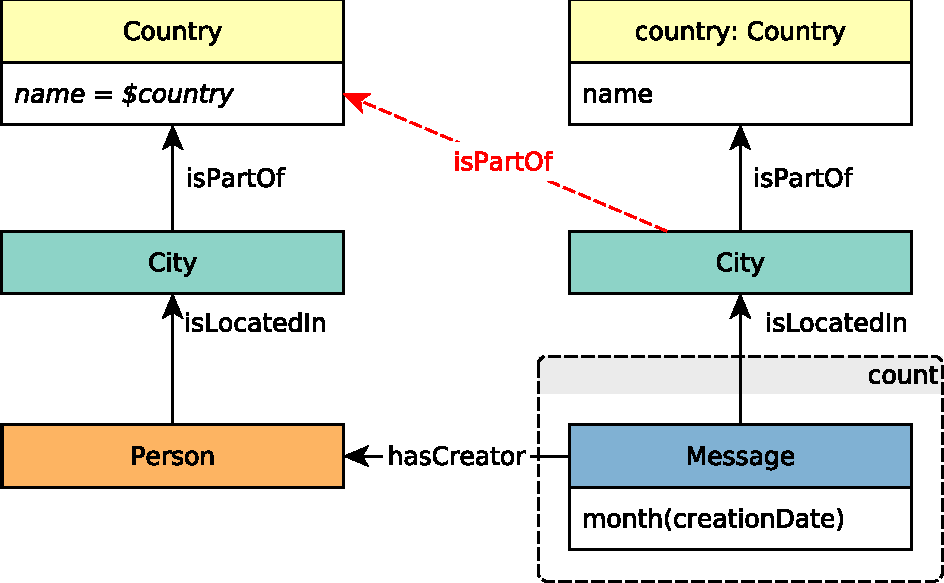
\includegraphics[scale=\patternscale,margin=0cm .2cm]{patterns/q23}
		\caption{Example graph pattern.}
		\label{fig:example-graph-pattern}
	\end{center}
\end{figure}



\section{Business Intelligence Queries}

\clearpage

\renewcommand*{\arraystretch}{1.1}

\noindent\begin{tabularx}{17cm}{|p{1.95cm}|X|}
	\hline
	workload    & BI \\ \hline
%
	query       & 1 \\ \hline
%
	title       & Posting summary \\ \hline
	\multicolumn{2}{|c|}{ 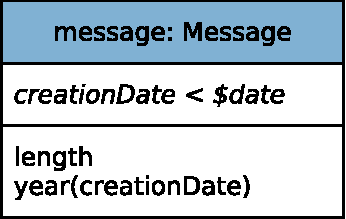
\includegraphics[scale=\patternscale,margin=0cm .2cm]{patterns/bi01}} \\ \hline
	description & Given a date, find all Messages created before that date. Group them by
a 3-level grouping:

\begin{enumerate}
\def\labelenumi{\arabic{enumi}.}
\tightlist
\item
  by year of creation
\item
  for each year, group into message types, i.e., Posts or Comments
\item
  for each year-type group, split into four groups based on length of
  their content

  \begin{itemize}
  \tightlist
  \item
    0 \textless{}= length \textless{} 40: \texttt{short}
  \item
    40 \textless{}= length \textless{} 80: \texttt{one\ liner}
  \item
    80 \textless{}= length \textless{} 160: \texttt{tweet}
  \item
    160 \textless{}= length: \texttt{long}
  \end{itemize}
\end{enumerate}
 \\ \hline
	
%
	group by       &
	\multicolumn{1}{>{\raggedright}X|}{
		\varname{year}, 
		\varname{message type}, 
		\varname{length group}
		} \\ \hline
	
%
	parameters  &
	\vspace{1.1ex}{\begin{tabularx}{14.2cm}{|c|M|m{2cm}|Y|} \hline
	\cellcolor{black!70} \color{white} $\mathsf{1}$ & \varname{date} & \cellcolor{gray!20} \vartype{Date} &  \\ \hline
	\end{tabularx}}\vspace{1.1ex} \\ \hline
%
	result      &
	\vspace{1.1ex}{\begin{tabularx}{14.2cm}{|c|M|m{2cm}|Y|} \hline
	\cellcolor{black!70} \color{white} $\mathsf{1}$ & \varname{message.year} & \cellcolor{gray!20} \vartype{32-bit Integer} &  \\ \hline
	\cellcolor{black!70} \color{white} $\mathsf{2}$ & \varname{messageType} & \cellcolor{gray!20} \vartype{String} & post/comment (in lowercase) \\ \hline
	\cellcolor{black!70} \color{white} $\mathsf{3}$ & \varname{lengthCategory} & \cellcolor{gray!20} \vartype{String} & short/one-liner/tweet/long (in lowercase) \\ \hline
	\cellcolor{black!70} \color{white} $\mathsf{4}$ & \varname{messageCount} & \cellcolor{gray!20} \vartype{32-bit Integer} & total number of Messages (Posts/Comments) in that group \\ \hline
	\cellcolor{black!70} \color{white} $\mathsf{5}$ & \varname{averageMessageLength} & \cellcolor{gray!20} \vartype{32-bit Integer} & average length of the Message content in that group \\ \hline
	\cellcolor{black!70} \color{white} $\mathsf{6}$ & \varname{sumMessageLength} & \cellcolor{gray!20} \vartype{32-bit Integer} & sum of all message content lengths \\ \hline
	\cellcolor{black!70} \color{white} $\mathsf{7}$ & \varname{percentageOfMessages} & \cellcolor{gray!20} \vartype{32-bit Float} & number of messages in group as a percentage of all messages created before the given date \\ \hline
	\end{tabularx}}\vspace{1.1ex} \\ \hline
	%
	sort        &
	\vspace{1.1ex}{\begin{tabular}{|c|l|c|} \hline
	\cellcolor{black!70} \color{white} $\mathsf{1}$ & \varname{year} & \cellcolor{gray!20} $\desc$ \\ \hline
	\cellcolor{black!70} \color{white} $\mathsf{2}$ & \varname{message type} & \cellcolor{gray!20} $\asc$ \\ \hline
	\cellcolor{black!70} \color{white} $\mathsf{3}$ & \varname{size category} & \cellcolor{gray!20} $\asc$ \\ \hline
	\end{tabular}}\vspace{1.1ex} \\ \hline
	%
	%
	choke points &
	\multicolumn{1}{>{\raggedright}X|}{
		\chokepoint{1.2}, 
		\chokepoint{3.2}, 
		\chokepoint{4.1}
		}\\ \hline
\end{tabularx}
\clearpage
\renewcommand*{\arraystretch}{1.5}
\noindent\begin{tabularx}{17cm}{|p{1.95cm}|X|}
	\hline
	number      & 2                                                          \\ \hline
	title       & Top tags for country, age, gender, time                                                           \\ \hline
	\multicolumn{2}{|c|}{ 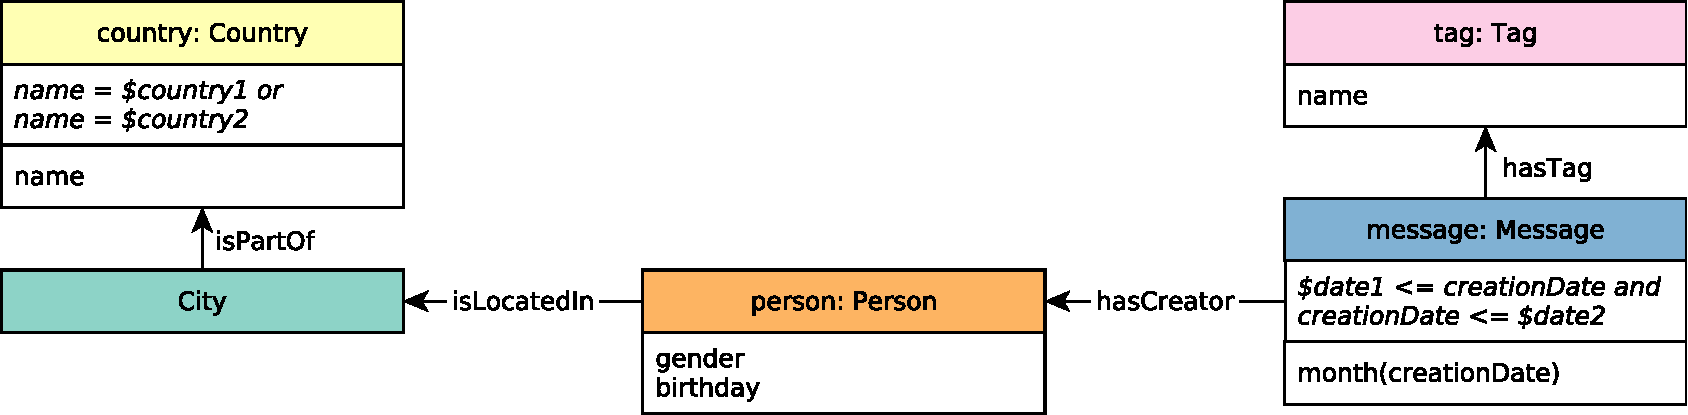
\includegraphics[scale=\patternscale,margin=0cm .2cm]{patterns/q02}} \\ \hline
	description & Select all Messages (Posts \& Comments) created between date1-date2
(inclusive) by persons located in country1 or country2. Select the
creators (Persons) and the Tags of these Messages. Split these Persons,
Tags and Messages into a 5-level grouping: (1) name of country of
person, (2) month message was created, (3) gender of person, (4) age
group of person, defined as years between person's birthday and end of
simulation (2013-01-01), divided by 5, rounded down, (5) name of tag
attached to message.

Only return groups where number of messages is greater than 100.
 \\ \hline
	
	group by       &
	\multicolumn{1}{>{\raggedright}X|}{
		\varname{countryName}, 
		\varname{month}, 
		\varname{gender}, 
		\varname{ageGroup}, 
		\varname{tagName}
		}\\ \hline
	
	parameters  &
	\renewcommand*{\arraystretch}{1.0}
	\vspace{-1.8ex}{\begin{tabularx}{14.2cm}{|c|l|p{2cm}|Y|} \hline
	\cellcolor{black!70} \color{white} $\mathsf{1}$ & \varname{date1} & \cellcolor{gray!20} \vartype{Date} & \\ \hline
	\cellcolor{black!70} \color{white} $\mathsf{2}$ & \varname{date2} & \cellcolor{gray!20} \vartype{Date} & \\ \hline
	\cellcolor{black!70} \color{white} $\mathsf{3}$ & \varname{country1} & \cellcolor{gray!20} \vartype{String} & \\ \hline
	\cellcolor{black!70} \color{white} $\mathsf{4}$ & \varname{country2} & \cellcolor{gray!20} \vartype{String} & \\ 
	\end{tabularx}} \\ \hline
	result      &
	\renewcommand*{\arraystretch}{1.0}
	\vspace{-1.8ex}{\begin{tabularx}{14.2cm}{|c|l|p{2cm}|Y|} \hline
	\cellcolor{black!70} \color{white} $\mathsf{1}$ & \varname{country.name} & \cellcolor{gray!20} \vartype{String} & \\ \hline
	\cellcolor{black!70} \color{white} $\mathsf{2}$ & \varname{message.month} & \cellcolor{gray!20} \vartype{32bitInteger} & \\ \hline
	\cellcolor{black!70} \color{white} $\mathsf{3}$ & \varname{person.gender} & \cellcolor{gray!20} \vartype{String} & \\ \hline
	\cellcolor{black!70} \color{white} $\mathsf{4}$ & \varname{ageGroup} & \cellcolor{gray!20} \vartype{32bitInteger} & \\ \hline
	\cellcolor{black!70} \color{white} $\mathsf{5}$ & \varname{tag.name} & \cellcolor{gray!20} \vartype{String} & \\ \hline
	\cellcolor{black!70} \color{white} $\mathsf{6}$ & \varname{messageCount} & \cellcolor{gray!20} \vartype{64bitInteger} & \\ 
	\end{tabularx}} \\ \hline
	sort        &
	\renewcommand*{\arraystretch}{1.0}
	\vspace{-1.8ex}{\begin{tabular}{|c|l|c|} \hline
	\cellcolor{black!70} \color{white} $\mathsf{1}$ & \varname{messageCount} & \cellcolor{gray!20} $\desc$ \\ \hline
	\cellcolor{black!70} \color{white} $\mathsf{2}$ & \varname{tag.name} & \cellcolor{gray!20} $\asc$ \\ \hline
	\cellcolor{black!70} \color{white} $\mathsf{3}$ & \varname{ageGroup} & \cellcolor{gray!20} $\asc$ \\ \hline
	\cellcolor{black!70} \color{white} $\mathsf{4}$ & \varname{person.gender} & \cellcolor{gray!20} $\asc$ \\ \hline
	\cellcolor{black!70} \color{white} $\mathsf{5}$ & \varname{message.month} & \cellcolor{gray!20} $\asc$ \\ \hline
	\cellcolor{black!70} \color{white} $\mathsf{6}$ & \varname{country.name} & \cellcolor{gray!20} $\asc$ \\ 
	\end{tabular}} \\ \hline
	limit       & 100                                                           \\ \hline
	choke points        &
	\multicolumn{1}{>{\raggedright}X|}{
		\chokepoint{1.1}, 
		\chokepoint{1.2}, 
		\chokepoint{1.4}, 
		\chokepoint{2.1}, 
		\chokepoint{2.3}, 
		\chokepoint{3.1}, 
		\chokepoint{3.2}
		}\\ \hline
\end{tabularx}
\clearpage
\renewcommand*{\arraystretch}{1.1}

\noindent\begin{tabularx}{17cm}{|p{1.95cm}|X|}
	\hline
	workload    & BI \\ \hline
%
	query       & 3 \\ \hline
%
	title       & Tag evolution \\ \hline
	\multicolumn{2}{|c|}{ 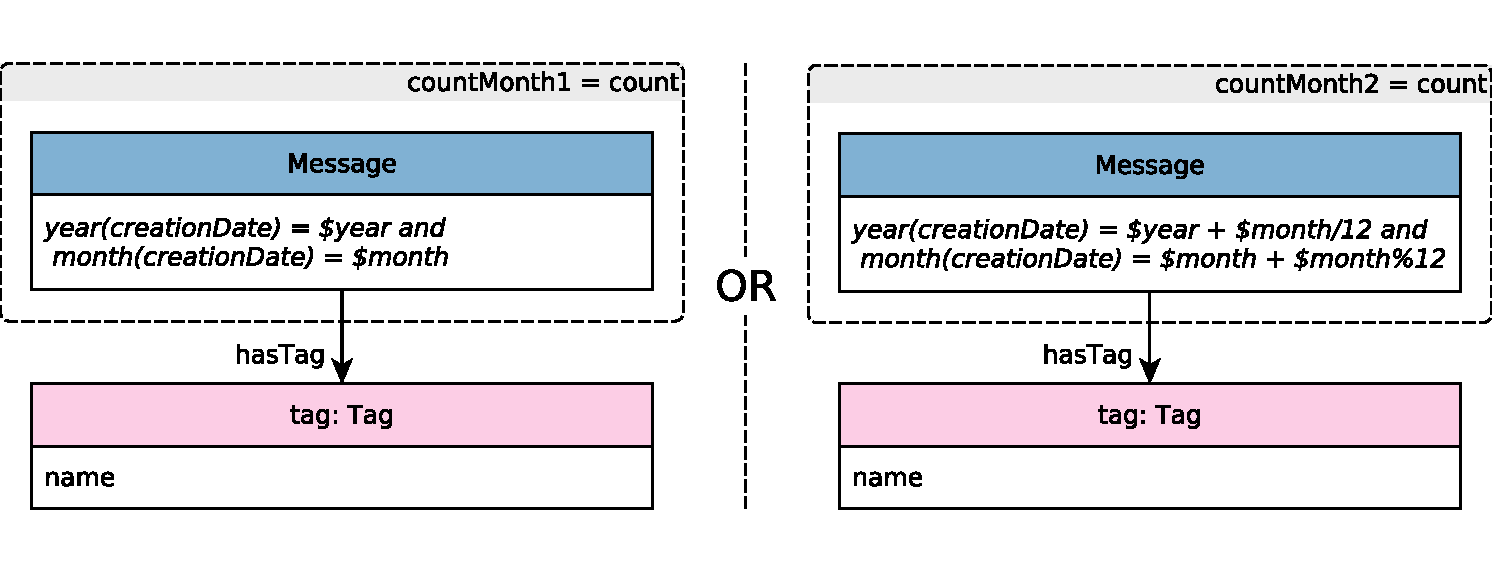
\includegraphics[scale=\patternscale,margin=0cm .2cm]{patterns/bi03}} \\ \hline
	description & Given a year and a month, find the Tags that were used in Messages
during the given month of the given year, and the Tags that were used
during the month after the given month of the given year.

For both months, compute the count of Messages that used each of the
Tags.
 \\ \hline
	
%
	parameters  &
	\vspace{1.1ex}{\begin{tabularx}{14.38cm}{|c|M|m{2cm}|Y} \hline
	\cellcolor{black!70} \color{white} $\mathsf{1}$ & \varname{year} & \cellcolor{gray!20} \vartype{32-bit Integer} &  \\\hline
	\cellcolor{black!70} \color{white} $\mathsf{2}$ & \varname{month} & \cellcolor{gray!20} \vartype{32-bit Integer} &  \\
	\end{tabularx}} \\ \hline
%
	result      &
	\vspace{1.1ex}{\begin{tabularx}{14.38cm}{|c|M|m{2cm}|Y} \hline
	\cellcolor{black!70} \color{white} $\mathsf{1}$ & \varname{tag.name} & \cellcolor{gray!20} \vartype{String} &  \\\hline
	\cellcolor{black!70} \color{white} $\mathsf{2}$ & \varname{countMonth1} & \cellcolor{gray!20} \vartype{32-bit Integer} & occurrences of the tag during year-month 1 \\\hline
	\cellcolor{black!70} \color{white} $\mathsf{3}$ & \varname{countMonth2} & \cellcolor{gray!20} \vartype{32-bit Integer} & occurrences of the tag during year-month 2 \\\hline
	\cellcolor{black!70} \color{white} $\mathsf{4}$ & \varname{diff} & \cellcolor{gray!20} \vartype{32-bit Integer} & difference between occurrences of this Tag in month 1 and month 2 \\
	\end{tabularx}} \\ \hline
	%
	sort        &
	\vspace{1.1ex}{\begin{tabular}{|c|l|c|} \hline
	\cellcolor{black!70} \color{white} $\mathsf{1}$ & \varname{diff} & \cellcolor{gray!20} $\desc$ \\\hline
	\cellcolor{black!70} \color{white} $\mathsf{2}$ & \varname{tag.name} & \cellcolor{gray!20} $\asc$ \\
	\end{tabular}} \\ \hline
	%
	limit       & 100 \\ \hline
	%
	choke points &
	\multicolumn{1}{>{\raggedright}X|}{
		\chokepoint{2.4}, 
		\chokepoint{3.1}, 
		\chokepoint{3.2}, 
		\chokepoint{4.1}, 
		\chokepoint{4.3}, 
		\chokepoint{5.3}, 
		\chokepoint{6.1}
		}\\ \hline
\end{tabularx}
\clearpage
\renewcommand*{\arraystretch}{1.1}

\noindent\begin{tabularx}{17cm}{|p{1.95cm}|X|}
	\hline
	workload    & BI \\ \hline
%
	query       & 4 \\ \hline
%
	title       & Popular topics in a country \\ \hline
	\multicolumn{2}{|c|}{ 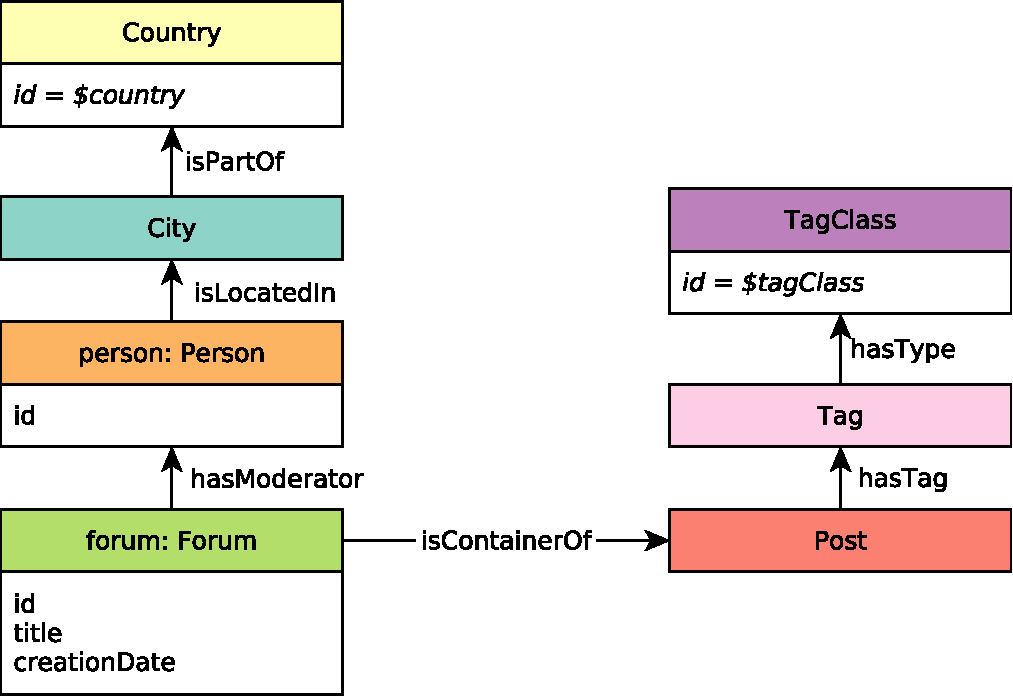
\includegraphics[scale=\patternscale,margin=0cm .2cm]{patterns/bi04}} \\ \hline
	description & Given a TagClass and a Country, find all the Forums created in the given
Country, containing at least one Post with Tags belonging directly to
the given TagClass.

The location of a Forum is identified by the location of the Forum's
moderator.

TODO - what do we count, Posts? (szarnyasg)
 \\ \hline
	
%
	parameters  &
	\vspace{1.1ex}{\begin{tabularx}{14.38cm}{|c|M|m{2cm}|Y} \hline
	\cellcolor{black!70} \color{white} $\mathsf{1}$ & \varname{tagClass} & \cellcolor{gray!20} \vartype{32-bit Integer} &  \\\hline
	\cellcolor{black!70} \color{white} $\mathsf{2}$ & \varname{country} & \cellcolor{gray!20} \vartype{32-bit Integer} &  \\
	\end{tabularx}} \\ \hline
%
	result      &
	\vspace{1.1ex}{\begin{tabularx}{14.38cm}{|c|M|m{2cm}|Y} \hline
	\cellcolor{black!70} \color{white} $\mathsf{1}$ & \varname{forum.id} & \cellcolor{gray!20} \vartype{64-bit Integer} &  \\\hline
	\cellcolor{black!70} \color{white} $\mathsf{2}$ & \varname{forum.title} & \cellcolor{gray!20} \vartype{String} &  \\\hline
	\cellcolor{black!70} \color{white} $\mathsf{3}$ & \varname{forum.creationDate} & \cellcolor{gray!20} \vartype{DateTime} &  \\\hline
	\cellcolor{black!70} \color{white} $\mathsf{4}$ & \varname{person.id} & \cellcolor{gray!20} \vartype{64-bit Integer} &  \\\hline
	\cellcolor{black!70} \color{white} $\mathsf{5}$ & \varname{count} & \cellcolor{gray!20} \vartype{32-bit Integer} &  \\
	\end{tabularx}} \\ \hline
	%
	sort        &
	\vspace{1.1ex}{\begin{tabular}{|c|l|c|} \hline
	\cellcolor{black!70} \color{white} $\mathsf{1}$ & \varname{count} & \cellcolor{gray!20} $\desc$ \\\hline
	\cellcolor{black!70} \color{white} $\mathsf{2}$ & \varname{forum.id} & \cellcolor{gray!20} $\asc$ \\
	\end{tabular}} \\ \hline
	%
	limit       & 20 \\ \hline
	%
	choke points &
	\multicolumn{1}{>{\raggedright}X|}{
		\chokepoint{1.1}, 
		\chokepoint{1.2}, 
		\chokepoint{1.4}, 
		\chokepoint{2.1}, 
		\chokepoint{2.2}, 
		\chokepoint{2.4}, 
		\chokepoint{3.3}
		}\\ \hline
\end{tabularx}
\clearpage
\renewcommand*{\arraystretch}{1.1}

\noindent\begin{tabularx}{17cm}{|p{1.95cm}|X|}
	\hline
	workload    & BI \\ \hline
%
	query       & 5 \\ \hline
%
	title       & Top posters in a country \\ \hline
	\multicolumn{2}{|c|}{ 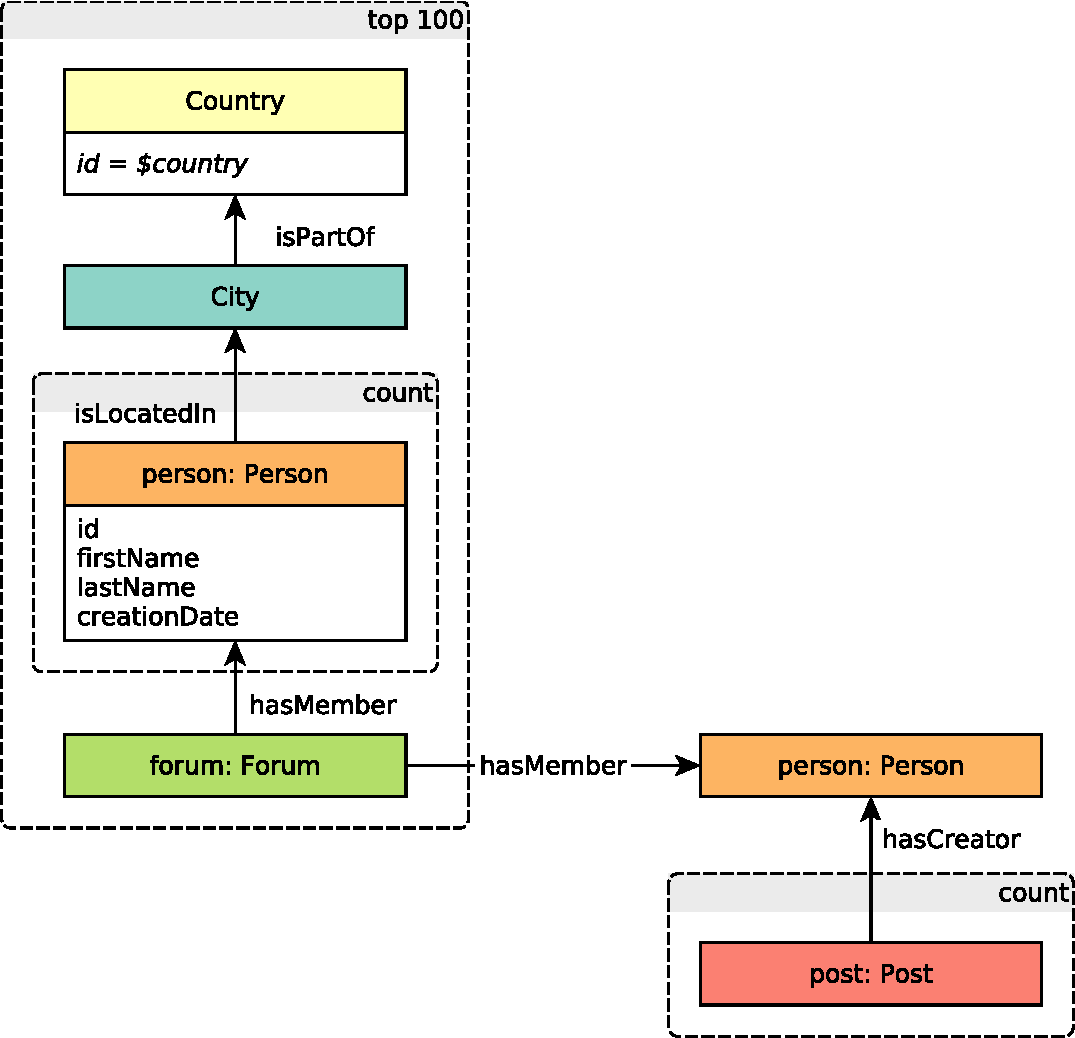
\includegraphics[scale=\patternscale,margin=0cm .2cm]{patterns/bi05}} \\ \hline
	description & Find the most popular Forums for a given Country, where the popularity
of a Forum is measured by the number of members that Forum has from the
given Country.

For each member of the 100 most popular Forums, count the number of
Posts they made in any of those (most popular) Forums.
 \\ \hline
	
%
	group by       &
	\multicolumn{1}{>{\raggedright}X|}{
		\varname{person.id}, 
		\varname{person.firstName}, 
		\varname{person.lastName}, 
		\varname{person.creationDate}
		} \\ \hline
	
%
	parameters  &
	\vspace{1.1ex}{\begin{tabularx}{14.2cm}{|c|M|m{2cm}|Y|} \hline
	\cellcolor{black!70} \color{white} $\mathsf{1}$ & \varname{country} & \cellcolor{gray!20} \vartype{32-bit Integer} &  \\ \hline
	\end{tabularx}}\vspace{1.1ex} \\ \hline
%
	result      &
	\vspace{1.1ex}{\begin{tabularx}{14.2cm}{|c|M|m{2cm}|Y|} \hline
	\cellcolor{black!70} \color{white} $\mathsf{1}$ & \varname{person.id} & \cellcolor{gray!20} \vartype{64-bit Integer} &  \\ \hline
	\cellcolor{black!70} \color{white} $\mathsf{2}$ & \varname{person.firstName} & \cellcolor{gray!20} \vartype{String} &  \\ \hline
	\cellcolor{black!70} \color{white} $\mathsf{3}$ & \varname{person.lastName} & \cellcolor{gray!20} \vartype{String} &  \\ \hline
	\cellcolor{black!70} \color{white} $\mathsf{4}$ & \varname{person.creationDate} & \cellcolor{gray!20} \vartype{DateTime} &  \\ \hline
	\cellcolor{black!70} \color{white} $\mathsf{5}$ & \varname{postCount} & \cellcolor{gray!20} \vartype{32-bit Integer} &  \\ \hline
	\end{tabularx}}\vspace{1.1ex} \\ \hline
	%
	sort        &
	\vspace{1.1ex}{\begin{tabular}{|c|l|c|} \hline
	\cellcolor{black!70} \color{white} $\mathsf{1}$ & \varname{postCount} & \cellcolor{gray!20} $\desc$ \\ \hline
	\cellcolor{black!70} \color{white} $\mathsf{2}$ & \varname{person.id} & \cellcolor{gray!20} $\asc$ \\ \hline
	\end{tabular}}\vspace{1.1ex} \\ \hline
	%
	limit       & 100 \\ \hline
	%
	choke points &
	\multicolumn{1}{>{\raggedright}X|}{
		\chokepoint{1.2}, 
		\chokepoint{1.4}, 
		\chokepoint{1.5}, 
		\chokepoint{2.1}, 
		\chokepoint{2.2}, 
		\chokepoint{2.3}, 
		\chokepoint{2.4}, 
		\chokepoint{3.3}, 
		\chokepoint{5.3}, 
		\chokepoint{6.1}
		}\\ \hline
\end{tabularx}
\clearpage
\renewcommand*{\arraystretch}{1.5}
\noindent\begin{tabularx}{17cm}{|p{1.95cm}|X|}
	\hline
	number      & 6                                                          \\ \hline
	title       & Most active Posters of a given Topic                                                           \\ \hline
	\multicolumn{2}{|c|}{ 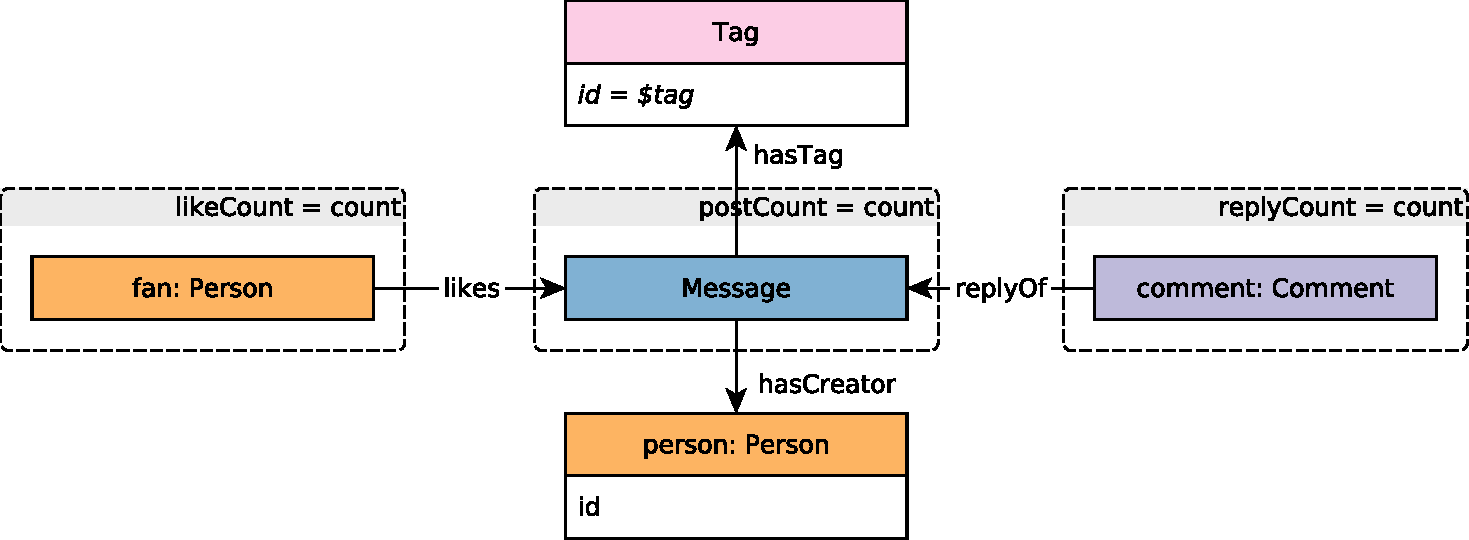
\includegraphics[scale=\patternscale,margin=0cm .2cm]{patterns/q06}} \\ \hline
	description & Get Persons who have created a Message (Post or Comment) with a given
Tag.

Each Person has a score, computed as follows:

\begin{itemize}
\tightlist
\item
  Count of Messages with the given Tag (\texttt{postCount}).
\item
  Count of Likes (\texttt{likeCount}) and Comments (\texttt{replyCount})
  in reply of their Messages with the given Tag. (TODO - transitive or
  direct? szarnyasg)
\end{itemize}

The sum is weighted as follows:

\begin{itemize}
\tightlist
\item
  Messages (\texttt{postCount}) are multiplied by 1,
\item
  Comments to Messages (\texttt{replyCount}) are multiplied by 2,
\item
  Likes (\texttt{likeCount}) are multiplied by 10.
\end{itemize}
 \\ \hline
	
	parameters  &
	\renewcommand*{\arraystretch}{1.0}
	\vspace{-1.8ex}{\begin{tabularx}{14.2cm}{|c|l|p{2cm}|Y|} \hline
	\cellcolor{black!70} \color{white} $\mathsf{1}$ & \varname{tag} & \cellcolor{gray!20} \vartype{32bitInteger} & \\ 
	\end{tabularx}} \\ \hline
	result      &
	\renewcommand*{\arraystretch}{1.0}
	\vspace{-1.8ex}{\begin{tabularx}{14.2cm}{|c|l|p{2cm}|Y|} \hline
	\cellcolor{black!70} \color{white} $\mathsf{1}$ & \varname{person.id} & \cellcolor{gray!20} \vartype{64bitInteger} & \\ \hline
	\cellcolor{black!70} \color{white} $\mathsf{2}$ & \varname{replyCount} & \cellcolor{gray!20} \vartype{32bitInteger} & \\ \hline
	\cellcolor{black!70} \color{white} $\mathsf{3}$ & \varname{likeCount} & \cellcolor{gray!20} \vartype{32bitInteger} & \\ \hline
	\cellcolor{black!70} \color{white} $\mathsf{4}$ & \varname{postCount} & \cellcolor{gray!20} \vartype{32bitInteger} & \\ \hline
	\cellcolor{black!70} \color{white} $\mathsf{5}$ & \varname{score} & \cellcolor{gray!20} \vartype{32bitInteger} & \\ 
	\end{tabularx}} \\ \hline
	sort        &
	\renewcommand*{\arraystretch}{1.0}
	\vspace{-1.8ex}{\begin{tabular}{|c|l|c|} \hline
	\cellcolor{black!70} \color{white} $\mathsf{1}$ & \varname{score} & \cellcolor{gray!20} $\desc$ \\ \hline
	\cellcolor{black!70} \color{white} $\mathsf{2}$ & \varname{person.id} & \cellcolor{gray!20} $\asc$ \\ 
	\end{tabular}} \\ \hline
	limit       & 100                                                           \\ \hline
	choke points        &
	\multicolumn{1}{>{\raggedright}X|}{
		\chokepoint{1.2}, 
		\chokepoint{2.3}
		}\\ \hline
\end{tabularx}
\clearpage
\renewcommand*{\arraystretch}{1.1}

\noindent\begin{tabularx}{17cm}{|p{1.95cm}|X|}
	\hline
	number      & 7                                                          \\ \hline
%
	title       & Most authoritative users on a given topic                                                           \\ \hline
	\multicolumn{2}{|c|}{ 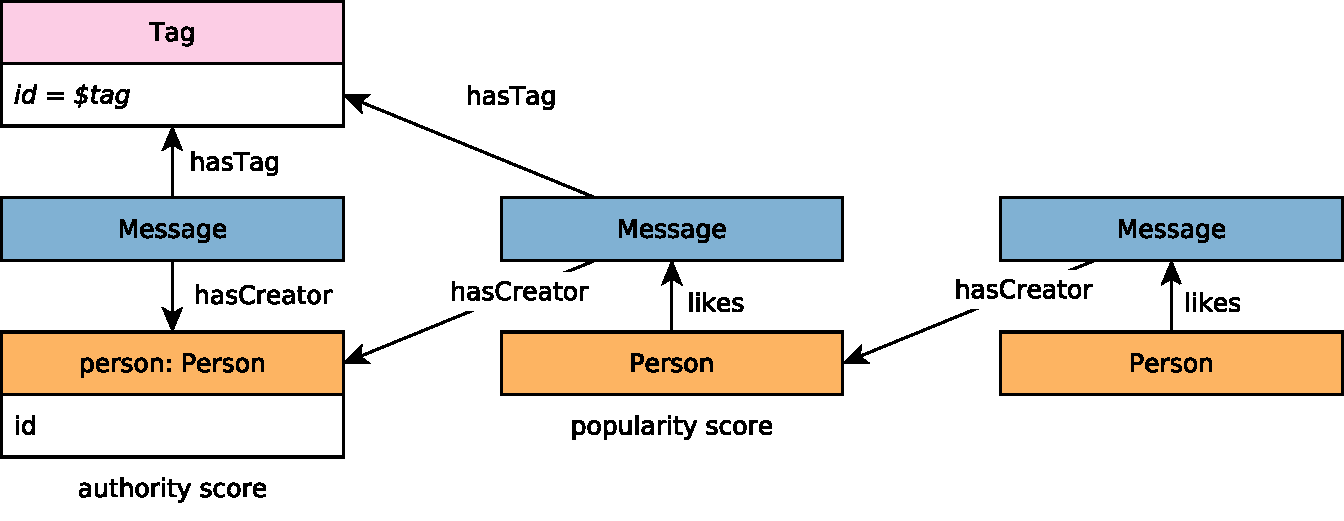
\includegraphics[scale=\patternscale,margin=0cm .2cm]{patterns/q07}} \\ \hline
	description & Given a Tag, find all Persons that ever created a Message with the given
Tag. For each of these Persons compute their ``authority score'' as
follows:

\begin{itemize}
\tightlist
\item
  The ``authority score'' is the sum of ``popularity scores'' of the
  Persons that liked any of that Person's Messages with the given Tag.
\item
  A Person's ``popularity score'' is defined as the total number of
  likes on all of their Messages.
\end{itemize}
 \\ \hline
	
%
	parameters  &
	\vspace{1.1ex}{\begin{tabularx}{14.2cm}{|c|l|m{2cm}|Y|} \hline
	\cellcolor{black!70} \color{white} $\mathsf{1}$ & \varname{tag} & \cellcolor{gray!20} \vartype{32-bit Integer} &  \\
	\end{tabularx}} \\ \hline
%
	result      &
	\vspace{1.1ex}{\begin{tabularx}{14.2cm}{|c|l|m{2cm}|Y|} \hline
	\cellcolor{black!70} \color{white} $\mathsf{1}$ & \varname{person1.id} & \cellcolor{gray!20} \vartype{64-bit Integer} &  \\\hline
	\cellcolor{black!70} \color{white} $\mathsf{2}$ & \varname{authorityScore} & \cellcolor{gray!20} \vartype{32-bit Integer} &  \\
	\end{tabularx}} \\ \hline
	%
	sort        &
	\vspace{1.1ex}{\begin{tabular}{|c|l|c|} \hline
	\cellcolor{black!70} \color{white} $\mathsf{1}$ & \varname{authorityScore} & \cellcolor{gray!20} $\desc$ \\\hline
	\cellcolor{black!70} \color{white} $\mathsf{2}$ & \varname{person1.id} & \cellcolor{gray!20} $\asc$ \\
	\end{tabular}} \\ \hline
	%
	limit       & 100 \\ \hline
	%
	choke points &
	\multicolumn{1}{>{\raggedright}X|}{
		\chokepoint{1.2}, 
		\chokepoint{2.3}, 
		\chokepoint{3.2}, 
		\chokepoint{3.3}, 
		\chokepoint{6.1}
		}\\ \hline
\end{tabularx}
\clearpage
\renewcommand*{\arraystretch}{1.1}

\noindent\begin{tabularx}{17cm}{|p{1.95cm}|X|}
	\hline
	workload    & BI \\ \hline
%
	query       & 8 \\ \hline
%
	title       & Related topics \\ \hline
%
    pattern     & \hfill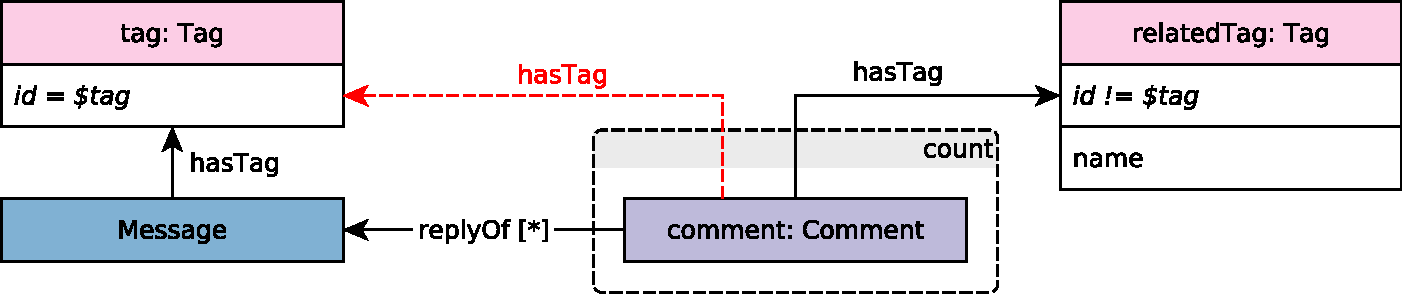
\includegraphics[scale=\patternscale,margin=0cm .2cm]{patterns/bi08}\hfill\vadjust{} \\ \hline
%
	description & Find all Messages that have a given Tag. Find the related Tags attached
to replies of these Messages (TODO - transitive? szarnyasg), but only of
those replies that do not have the given Tag.

Group the Tags by name, and get the count of replies in each group.
 \\ \hline
	
%
	group by       &
	\multicolumn{1}{>{\raggedright}X|}{
		\varname{relatedTag.name}
		} \\ \hline
	
%
	parameters  &
	\vspace{1.1ex}{\begin{tabularx}{14.2cm}{|c|M|m{2cm}|Y|} \hline
	\cellcolor{black!70} \color{white} $\mathsf{1}$ & \varname{tag} & \cellcolor{gray!20} \vartype{32-bit Integer} &  \\ \hline
	\end{tabularx}}\vspace{1.1ex} \\ \hline
%
	result      &
	\vspace{1.1ex}{\begin{tabularx}{14.2cm}{|c|M|m{2cm}|Y|} \hline
	\cellcolor{black!70} \color{white} $\mathsf{1}$ & \varname{relatedTag.name} & \cellcolor{gray!20} \vartype{String} &  \\ \hline
	\cellcolor{black!70} \color{white} $\mathsf{2}$ & \varname{count} & \cellcolor{gray!20} \vartype{32-bit Integer} &  \\ \hline
	\end{tabularx}}\vspace{1.1ex} \\ \hline
	%
	sort        &
	\vspace{1.1ex}{\begin{tabular}{|c|l|c|} \hline
	\cellcolor{black!70} \color{white} $\mathsf{1}$ & \varname{count} & \cellcolor{gray!20} $\desc$ \\ \hline
	\cellcolor{black!70} \color{white} $\mathsf{2}$ & \varname{relatedTag.name} & \cellcolor{gray!20} $\asc$ \\ \hline
	\end{tabular}}\vspace{1.1ex} \\ \hline
	%
	limit       & 100 \\ \hline
	%
	choke points &
	\multicolumn{1}{>{\raggedright}X|}{
		\chokepoint{1.6}, 
		\chokepoint{3.3}, 
		\chokepoint{5.2}
		}\\ \hline
\end{tabularx}
\clearpage
\renewcommand*{\arraystretch}{1.1}

\noindent\begin{tabularx}{17cm}{|p{1.95cm}|X|}
	\hline
	number      & 9                                                          \\ \hline
%
	title       & Forum with related Tags                                                           \\ \hline
	\multicolumn{2}{|c|}{ 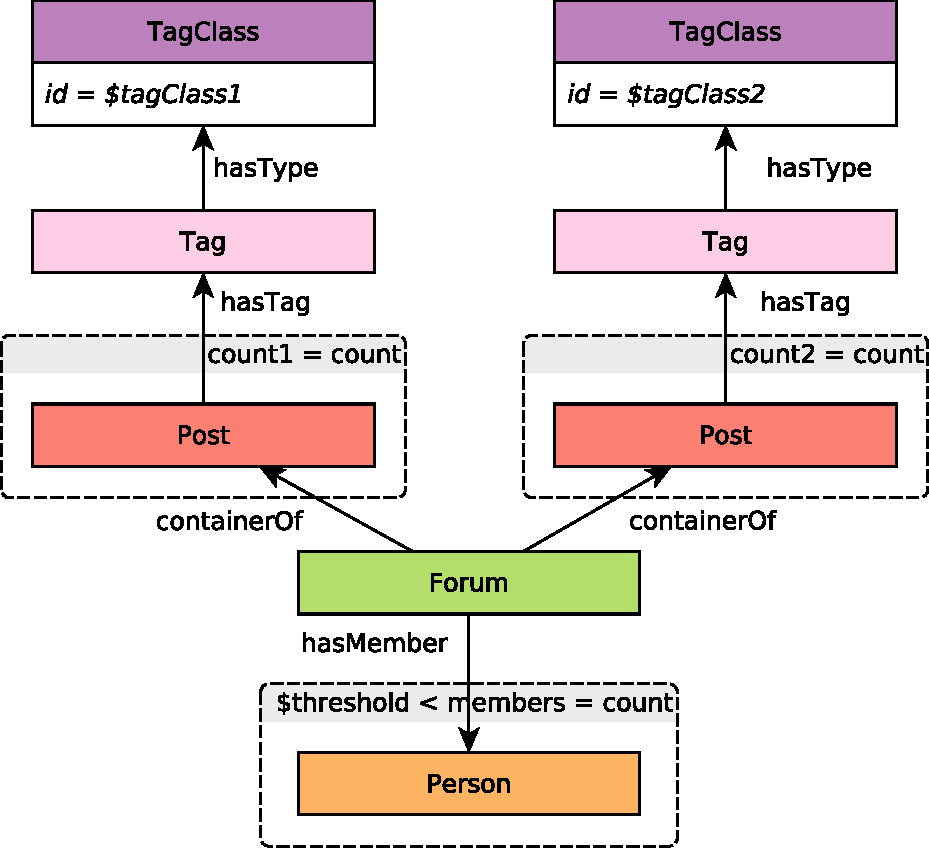
\includegraphics[scale=\patternscale,margin=0cm .2cm]{patterns/q09}} \\ \hline
	description & Given two TagClasses (\texttt{tagClass1} \& \texttt{tagClass2}), find
Forums that contain at least one Post with a Tag from \texttt{tagClass1}
and at least one Post with a Tag from \texttt{tagClass2} (direct
children not transitive) -- this may be the same Post.

Consider the Forums with a number of members greater than a given
threshold. For every such forum, count the number of Posts that have a
Tag from TagClass1 (count1), and the number of posts that have a tag
from TagClass2.
 \\ \hline
	
%
	parameters  &
	\vspace{1.1ex}{\begin{tabularx}{14.38cm}{|c|M|m{2cm}|Y} \hline
	\cellcolor{black!70} \color{white} $\mathsf{1}$ & \varname{tagClass1} & \cellcolor{gray!20} \vartype{32-bit Integer} &  \\\hline
	\cellcolor{black!70} \color{white} $\mathsf{2}$ & \varname{tagClass2} & \cellcolor{gray!20} \vartype{32-bit Integer} &  \\\hline
	\cellcolor{black!70} \color{white} $\mathsf{3}$ & \varname{threshold} & \cellcolor{gray!20} \vartype{32-bit Integer} &  \\
	\end{tabularx}} \\ \hline
%
	result      &
	\vspace{1.1ex}{\begin{tabularx}{14.38cm}{|c|M|m{2cm}|Y} \hline
	\cellcolor{black!70} \color{white} $\mathsf{1}$ & \varname{forum.id} & \cellcolor{gray!20} \vartype{64-bit Integer} &  \\\hline
	\cellcolor{black!70} \color{white} $\mathsf{2}$ & \varname{count1} & \cellcolor{gray!20} \vartype{32-bit Integer} & Number of Posts with at least one tag belonging to tagClass1 \\\hline
	\cellcolor{black!70} \color{white} $\mathsf{3}$ & \varname{count2} & \cellcolor{gray!20} \vartype{32-bit Integer} & Number of Posts with at least one tag belonging to tagClass2 \\
	\end{tabularx}} \\ \hline
	%
	sort        &
	\vspace{1.1ex}{\begin{tabular}{|c|l|c|} \hline
	\cellcolor{black!70} \color{white} $\mathsf{1}$ & \varname{count2} & \cellcolor{gray!20} $\desc$ \\\hline
	\cellcolor{black!70} \color{white} $\mathsf{2}$ & \varname{count1} & \cellcolor{gray!20} $\desc$ \\\hline
	\cellcolor{black!70} \color{white} $\mathsf{3}$ & \varname{forum.id} & \cellcolor{gray!20} $\asc$ \\
	\end{tabular}} \\ \hline
	%
	limit       & 100 \\ \hline
	%
	choke points &
	\multicolumn{1}{>{\raggedright}X|}{
		\chokepoint{1.2}, 
		\chokepoint{1.4}, 
		\chokepoint{2.1}, 
		\chokepoint{2.3}, 
		\chokepoint{2.4}
		}\\ \hline
\end{tabularx}
\clearpage
\renewcommand*{\arraystretch}{1.1}

\noindent\begin{tabularx}{17cm}{|p{1.95cm}|X|}
	\hline
	number      & 10                                                          \\ \hline
%
	title       & Central Person for a Tag                                                           \\ \hline
	\multicolumn{2}{|c|}{ 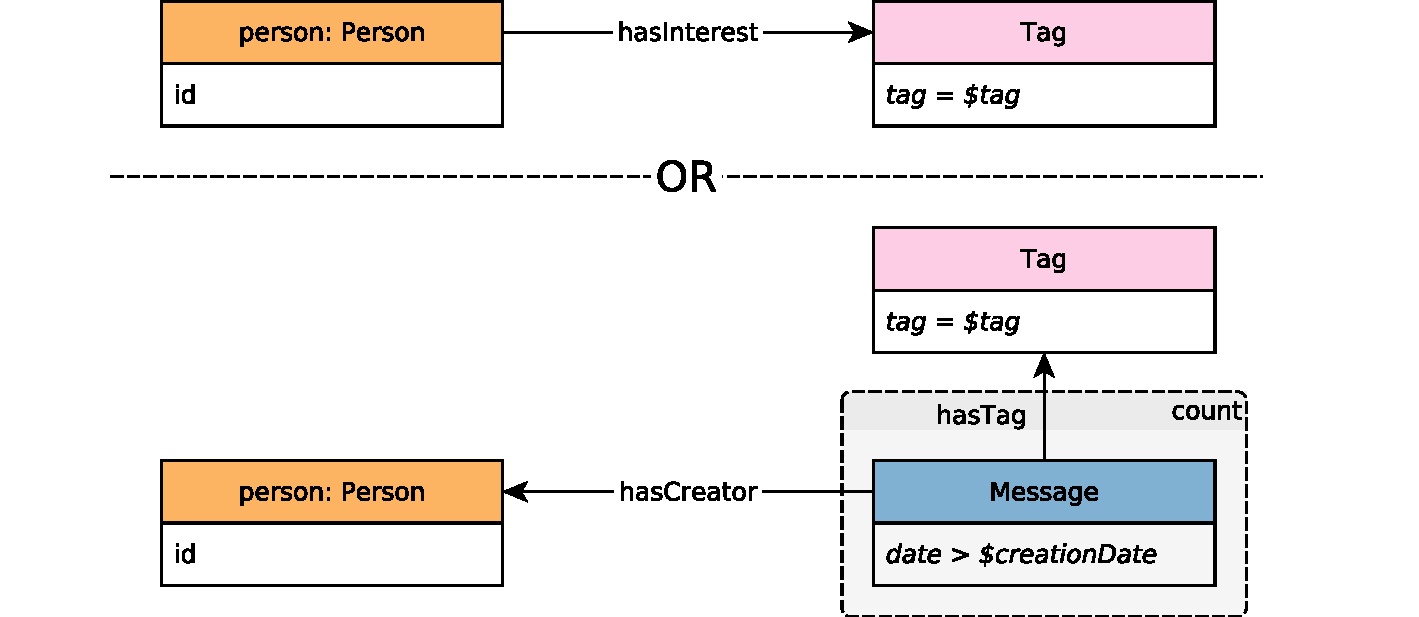
\includegraphics[scale=\patternscale,margin=0cm .2cm]{patterns/q10}} \\ \hline
	description & Given a Tag, find all Persons that are either interested in the Tag, or
have written a Message (Post or Comment) with creation date after a
given date and that has a given Tag. For each Person, compute the score
as the sum of the following two aspects:

\begin{itemize}
\tightlist
\item
  100, if the Person has this tag as their interest, or 0 otherwise
\item
  number of messages by this person with the given tag
\end{itemize}
 \\ \hline
	
%
	parameters  &
	\vspace{1.1ex}{\begin{tabularx}{14.2cm}{|c|l|m{2cm}|Y|} \hline
	\cellcolor{black!70} \color{white} $\mathsf{1}$ & \varname{tag} & \cellcolor{gray!20} \vartype{32-bit Integer} &  \\\hline
	\cellcolor{black!70} \color{white} $\mathsf{2}$ & \varname{date} & \cellcolor{gray!20} \vartype{Date} &  \\
	\end{tabularx}} \\ \hline
%
	result      &
	\vspace{1.1ex}{\begin{tabularx}{14.2cm}{|c|l|m{2cm}|Y|} \hline
	\cellcolor{black!70} \color{white} $\mathsf{1}$ & \varname{person.id} & \cellcolor{gray!20} \vartype{64-bit Integer} &  \\\hline
	\cellcolor{black!70} \color{white} $\mathsf{2}$ & \varname{score} & \cellcolor{gray!20} \vartype{32-bit Integer} &  \\\hline
	\cellcolor{black!70} \color{white} $\mathsf{3}$ & \varname{friendsScore} & \cellcolor{gray!20} \vartype{32-bit Integer} & The sum of the score of the Person's friends \\
	\end{tabularx}} \\ \hline
	%
	sort        &
	\vspace{1.1ex}{\begin{tabular}{|c|l|c|} \hline
	\cellcolor{black!70} \color{white} $\mathsf{1}$ & \varname{score + friendsScore} & \cellcolor{gray!20} $\desc$ \\\hline
	\cellcolor{black!70} \color{white} $\mathsf{2}$ & \varname{person.id} & \cellcolor{gray!20} $\asc$ \\
	\end{tabular}} \\ \hline
	%
	limit       & 100 \\ \hline
	%
	choke points &
	\multicolumn{1}{>{\raggedright}X|}{
		\chokepoint{1.2}, 
		\chokepoint{2.1}, 
		\chokepoint{2.3}, 
		\chokepoint{3.2}
		}\\ \hline
\end{tabularx}
\clearpage
\renewcommand*{\arraystretch}{1.5}
\begin{tabularx}{15cm}{|p{2.1cm}@{\hskip 1ex}|@{\hskip 1ex}X|}
	\hline
	number      & 11                                                          \\ \hline
	title       & Unrelated replies                                                           \\ \hline
	\multicolumn{2}{|c|}{ 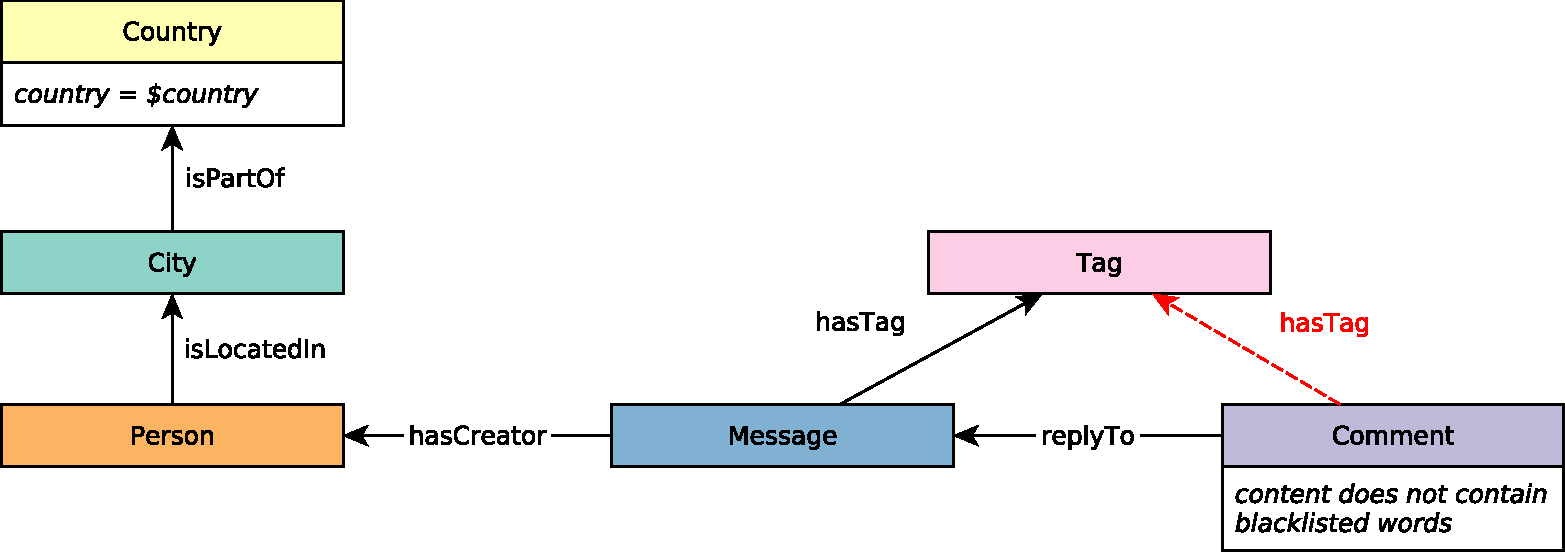
\includegraphics[scale=\patternscale,margin=0cm .2cm]{patterns/q11}} \\ \hline
	description & Find those Persons of a given country that replied to any Message, such
that the reply does not have any Tag in common with the Message {[}are
transitive replies considered or not? - SzG{]}. Consider only those
replies not containing any word from a given blacklist. For each Person
and valid reply, retrieve the Tags associated with the reply, and
retrieve the number of likes on the reply.
 \\ \hline
	
	group       &
	\multicolumn{1}{>{\raggedright}X|}{
		\varname{person.id}, 
		\varname{tag.name}
		}\\ \hline
	
	parameters  &
	\multicolumn{1}{>{\raggedright}X|}{
		\variable{country}{32bitInteger} \\
		\variable{blacklist}{String[]} 
		}\\ \hline
	result      &
	\multicolumn{1}{>{\raggedright}X|}{
		\variable{person.id}{64bitInteger}\\
		\variable{tag.name}{String}\\
		\variable{countLikes}{32bitInteger}The count of Likes to replies with that Tag.\\
		\variable{countReplies}{32bitInteger}The count of replies with that Tag.
		}\\ \hline
	sort        &
	\multicolumn{1}{>{\raggedright}X|}{
		\sortentry{countLikes}{\desc}\\
		\sortentry{person.id}{\asc}\\
		\sortentry{tag.name}{\asc}
		}\\ \hline
	limit       & 100                                                           \\ \hline
	choke points        &
	\multicolumn{1}{>{\raggedright}X|}{
		\chokepoint{1.1}, 
		\chokepoint{2.1}, 
		\chokepoint{2.2}, 
		\chokepoint{2.3}, 
		\chokepoint{3.1}, 
		\chokepoint{3.2}, 
		\chokepoint{6.1}
		}\\ \hline
\end{tabularx}
\clearpage

\renewcommand*{\arraystretch}{1.1}

\noindent\begin{tabularx}{17cm}{|p{1.95cm}|X|}
	\hline
	workload    & BI \\ \hline
%
	query       & 12 \\ \hline
%
	title       & Trending Posts \\ \hline
	\multicolumn{2}{|c|}{ 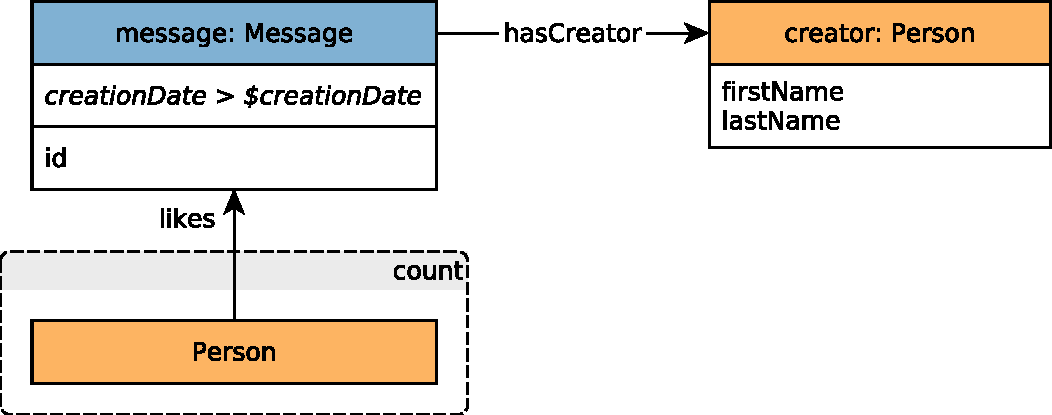
\includegraphics[scale=\patternscale,margin=0cm .2cm]{patterns/bi12}} \\ \hline
	description & Find all Messages created after a given date, that received more than a
given number of likes.
 \\ \hline
	
%
	parameters  &
	\vspace{1.1ex}{\begin{tabularx}{14.2cm}{|c|M|m{2cm}|Y|} \hline
	\cellcolor{black!70} \color{white} $\mathsf{1}$ & \varname{creationDate} & \cellcolor{gray!20} \vartype{Date} &  \\ \hline
	\cellcolor{black!70} \color{white} $\mathsf{2}$ & \varname{likeThreshold} & \cellcolor{gray!20} \vartype{32-bit Integer} &  \\ \hline
	\end{tabularx}}\vspace{1.1ex} \\ \hline
%
	result      &
	\vspace{1.1ex}{\begin{tabularx}{14.2cm}{|c|M|m{2cm}|Y|} \hline
	\cellcolor{black!70} \color{white} $\mathsf{1}$ & \varname{message.id} & \cellcolor{gray!20} \vartype{64-bit Integer} &  \\ \hline
	\cellcolor{black!70} \color{white} $\mathsf{2}$ & \varname{message.creationDate} & \cellcolor{gray!20} \vartype{DateTime} &  \\ \hline
	\cellcolor{black!70} \color{white} $\mathsf{3}$ & \varname{creator.firstName} & \cellcolor{gray!20} \vartype{String} & The first name of the post's creator \\ \hline
	\cellcolor{black!70} \color{white} $\mathsf{4}$ & \varname{creator.lastName} & \cellcolor{gray!20} \vartype{String} & The last name of the post's creator \\ \hline
	\cellcolor{black!70} \color{white} $\mathsf{5}$ & \varname{likeCount} & \cellcolor{gray!20} \vartype{32-bit Integer} & The number of Likes the Post received \\ \hline
	\end{tabularx}}\vspace{1.1ex} \\ \hline
	%
	sort        &
	\vspace{1.1ex}{\begin{tabular}{|c|l|c|} \hline
	\cellcolor{black!70} \color{white} $\mathsf{1}$ & \varname{likeCount} & \cellcolor{gray!20} $\desc$ \\ \hline
	\cellcolor{black!70} \color{white} $\mathsf{2}$ & \varname{message.id} & \cellcolor{gray!20} $\asc$ \\ \hline
	\end{tabular}}\vspace{1.1ex} \\ \hline
	%
	limit       & 100 \\ \hline
	%
	choke points &
	\multicolumn{1}{>{\raggedright}X|}{
		\chokepoint{1.2}, 
		\chokepoint{2.2}, 
		\chokepoint{3.1}, 
		\chokepoint{6.1}
		}\\ \hline
\end{tabularx}
\clearpage
\renewcommand*{\arraystretch}{1.1}

\noindent\begin{tabularx}{17cm}{|p{1.95cm}|X|}
	\hline
	workload    & BI \\ \hline
%
	query       & 13 \\ \hline
%
	title       & Popular Tags per month in a country \\ \hline
%
    pattern     & \hfill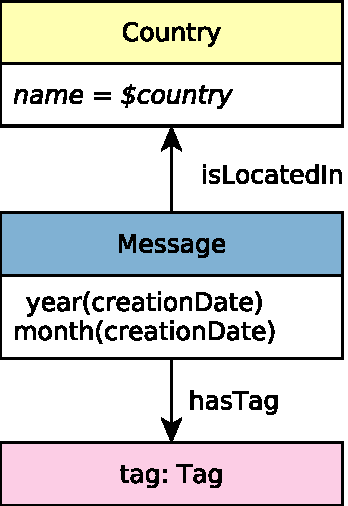
\includegraphics[scale=\patternscale,margin=0cm .2cm]{patterns/bi13}\hfill\vadjust{} \\ \hline
%
	description & Find all Messages in a given Country, as well as their Tags.

For each group, find the 5 most popular Tags, where popularity is the
number of Messages (from within the same group) where the Tag appears.
 \\ \hline
	
%
	group by       &
	\multicolumn{1}{>{\raggedright}X|}{
		\varname{year}, 
		\varname{month}
		} \\ \hline
	
%
	parameters  &
	\vspace{1.1ex}{\begin{tabularx}{14.2cm}{|c|M|m{2cm}|Y|} \hline
	\cellcolor{black!70} \color{white} $\mathsf{1}$ & \varname{country} & \cellcolor{gray!20} \vartype{String} &  \\ \hline
	\end{tabularx}}\vspace{1.1ex} \\ \hline
%
	result      &
	\vspace{1.1ex}{\begin{tabularx}{14.2cm}{|c|M|m{2cm}|Y|} \hline
	\cellcolor{black!70} \color{white} $\mathsf{1}$ & \varname{year} & \cellcolor{gray!20} \vartype{32-bit Integer} & year(message.creationDate) \\ \hline
	\cellcolor{black!70} \color{white} $\mathsf{2}$ & \varname{month} & \cellcolor{gray!20} \vartype{32-bit Integer} & month(message.creationDate) \\ \hline
	\cellcolor{black!70} \color{white} $\mathsf{3}$ & \varname{popularTags} & \cellcolor{gray!20} \vartype{TagPairs} & (tag.name - String, popularity - 32-bit Integer), sorted descending by popularity, then ascending by tag name \\ \hline
	\end{tabularx}}\vspace{1.1ex} \\ \hline
	%
	sort        &
	\vspace{1.1ex}{\begin{tabular}{|c|l|c|} \hline
	\cellcolor{black!70} \color{white} $\mathsf{1}$ & \varname{year} & \cellcolor{gray!20} $\desc$ \\ \hline
	\cellcolor{black!70} \color{white} $\mathsf{2}$ & \varname{month} & \cellcolor{gray!20} $\asc$ \\ \hline
	\end{tabular}}\vspace{1.1ex} \\ \hline
	%
	limit       & 100 \\ \hline
	%
	choke points &
	\multicolumn{1}{>{\raggedright}X|}{
		\chokepoint{1.2}, 
		\chokepoint{2.2}, 
		\chokepoint{2.3}, 
		\chokepoint{3.2}, 
		\chokepoint{6.1}
		}\\ \hline
\end{tabularx}
\clearpage
\renewcommand*{\arraystretch}{1.1}

\noindent\begin{tabularx}{17cm}{|p{1.95cm}|X|}
	\hline
	number      & 14                                                          \\ \hline
%
	title       & Top thread initiators                                                           \\ \hline
	\multicolumn{2}{|c|}{ 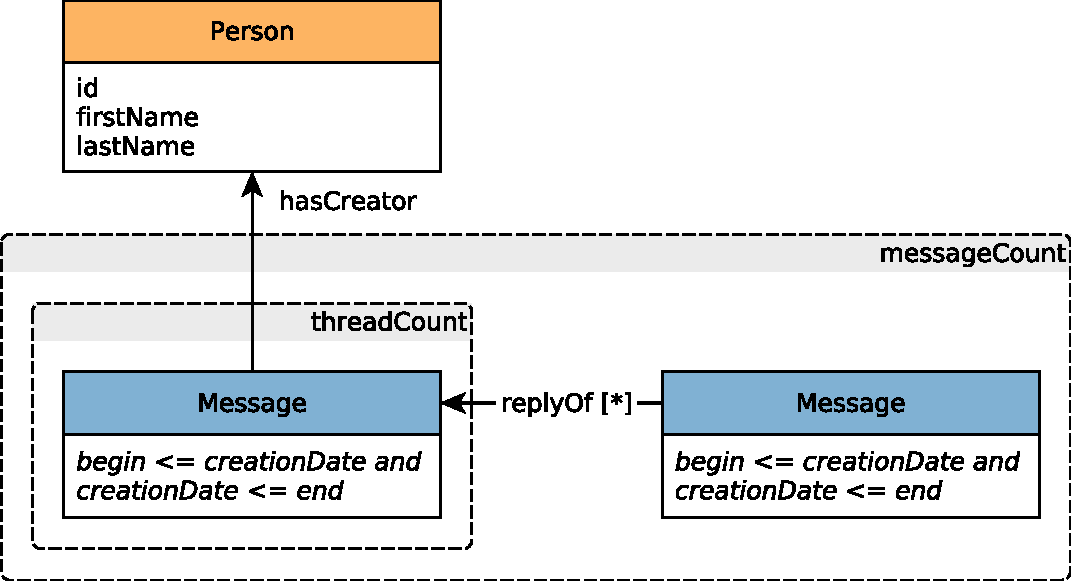
\includegraphics[scale=\patternscale,margin=0cm .2cm]{patterns/q14}} \\ \hline
	description & For each person, count the number Posts they created in the time
interval \texttt{(begin,\ end)}, and the number of messages in each of
their (transitive) reply trees. When calculating message counts only
consider messages created within the given time interval.

Return each person, number of Posts they created, and the count of all
messages that appeared in the reply trees (including Post at tree root)
they created.
 \\ \hline
	
%
	parameters  &
	\vspace{1.1ex}{\begin{tabularx}{14.38cm}{|c|M|m{2cm}|Y} \hline
	\cellcolor{black!70} \color{white} $\mathsf{1}$ & \varname{begin} & \cellcolor{gray!20} \vartype{Date} &  \\\hline
	\cellcolor{black!70} \color{white} $\mathsf{2}$ & \varname{end} & \cellcolor{gray!20} \vartype{Date} &  \\
	\end{tabularx}} \\ \hline
%
	result      &
	\vspace{1.1ex}{\begin{tabularx}{14.38cm}{|c|M|m{2cm}|Y} \hline
	\cellcolor{black!70} \color{white} $\mathsf{1}$ & \varname{person.id} & \cellcolor{gray!20} \vartype{64-bit Integer} &  \\\hline
	\cellcolor{black!70} \color{white} $\mathsf{2}$ & \varname{person.firstName} & \cellcolor{gray!20} \vartype{String} &  \\\hline
	\cellcolor{black!70} \color{white} $\mathsf{3}$ & \varname{person.lastName} & \cellcolor{gray!20} \vartype{String} &  \\\hline
	\cellcolor{black!70} \color{white} $\mathsf{4}$ & \varname{threadCount} & \cellcolor{gray!20} \vartype{32-bit Integer} & The number of threads initiated by that Person \\\hline
	\cellcolor{black!70} \color{white} $\mathsf{5}$ & \varname{messageCount} & \cellcolor{gray!20} \vartype{32-bit Integer} & The number of messages created in all the threads this Person initiated \\
	\end{tabularx}} \\ \hline
	%
	sort        &
	\vspace{1.1ex}{\begin{tabular}{|c|l|c|} \hline
	\cellcolor{black!70} \color{white} $\mathsf{1}$ & \varname{messageCount} & \cellcolor{gray!20} $\desc$ \\\hline
	\cellcolor{black!70} \color{white} $\mathsf{2}$ & \varname{person.id} & \cellcolor{gray!20} $\asc$ \\
	\end{tabular}} \\ \hline
	%
	limit       & 100 \\ \hline
	%
	choke points &
	\multicolumn{1}{>{\raggedright}X|}{
		\chokepoint{1.2}, 
		\chokepoint{2.2}, 
		\chokepoint{2.3}, 
		\chokepoint{3.2}, 
		\chokepoint{7.2}, 
		\chokepoint{7.3}, 
		\chokepoint{7.4}
		}\\ \hline
\end{tabularx}
\clearpage
\renewcommand*{\arraystretch}{1.1}

\noindent\begin{tabularx}{17cm}{|p{1.95cm}|X|}
	\hline
	workload    & bi \\ \hline
%
	query       & 15 \\ \hline
%
	title       & Social normals \\ \hline
	\multicolumn{2}{|c|}{ 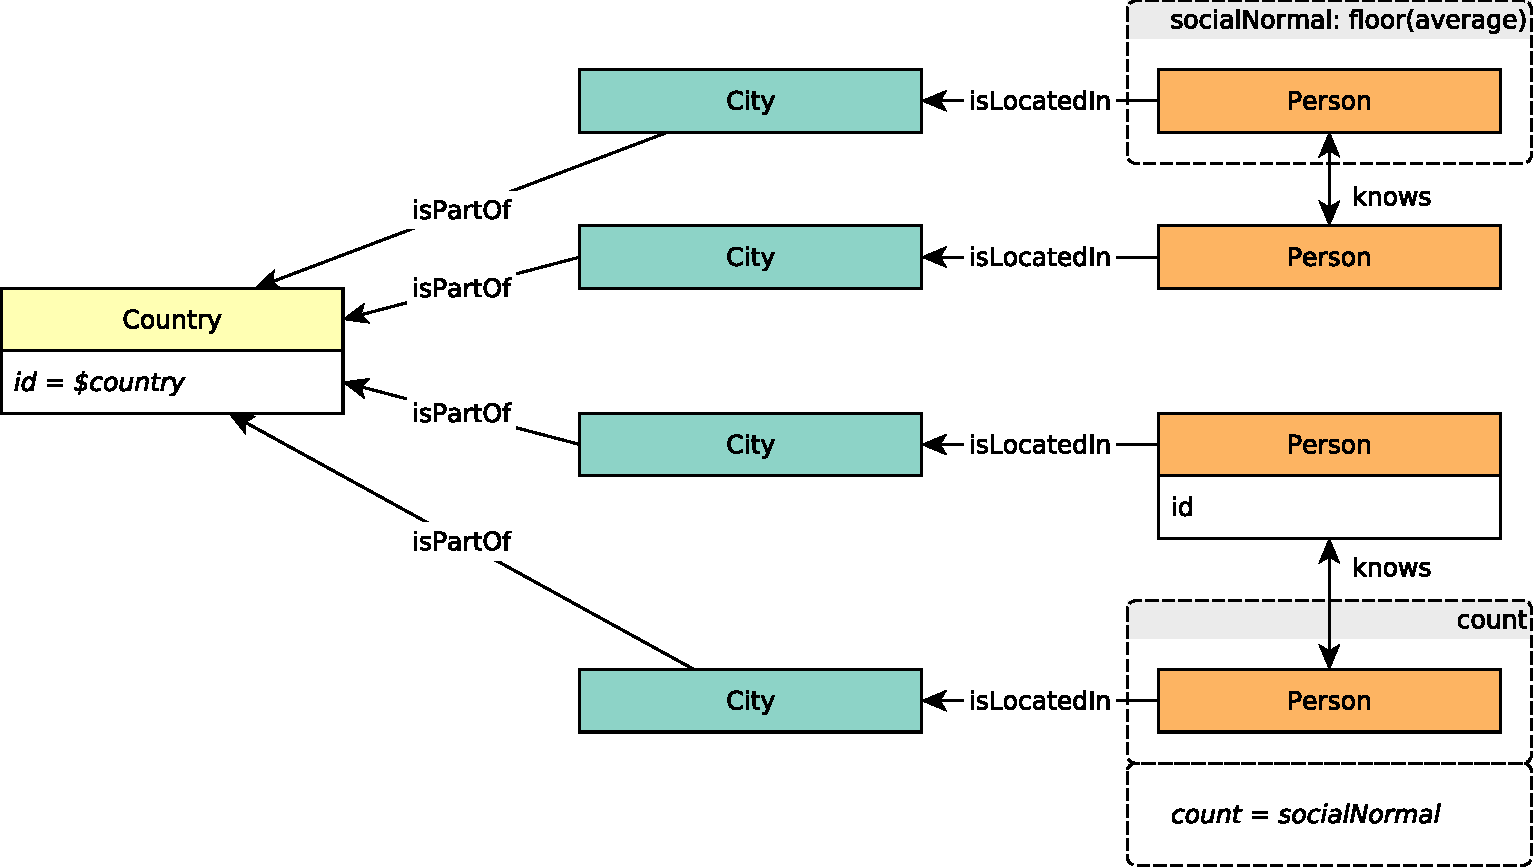
\includegraphics[scale=\patternscale,margin=0cm .2cm]{patterns/bi15}} \\ \hline
	description & Given a country, find all Persons of the country whose number of friends
in the given country equals the (floor of) average number of friends
that Persons of the given country have in the given country.
 \\ \hline
	
%
	parameters  &
	\vspace{1.1ex}{\begin{tabularx}{14.38cm}{|c|M|m{2cm}|Y} \hline
	\cellcolor{black!70} \color{white} $\mathsf{1}$ & \varname{country} & \cellcolor{gray!20} \vartype{32-bit Integer} &  \\
	\end{tabularx}} \\ \hline
%
	result      &
	\vspace{1.1ex}{\begin{tabularx}{14.38cm}{|c|M|m{2cm}|Y} \hline
	\cellcolor{black!70} \color{white} $\mathsf{1}$ & \varname{person.id} & \cellcolor{gray!20} \vartype{64-bit Integer} &  \\\hline
	\cellcolor{black!70} \color{white} $\mathsf{2}$ & \varname{count} & \cellcolor{gray!20} \vartype{32-bit Integer} &  \\
	\end{tabularx}} \\ \hline
	%
	sort        &
	\vspace{1.1ex}{\begin{tabular}{|c|l|c|} \hline
	\cellcolor{black!70} \color{white} $\mathsf{1}$ & \varname{person.id} & \cellcolor{gray!20} $\asc$ \\
	\end{tabular}} \\ \hline
	%
	limit       & 100 \\ \hline
	%
	choke points &
	\multicolumn{1}{>{\raggedright}X|}{
		\chokepoint{1.2}, 
		\chokepoint{2.3}, 
		\chokepoint{3.2}, 
		\chokepoint{3.3}, 
		\chokepoint{5.3}, 
		\chokepoint{6.1}
		}\\ \hline
\end{tabularx}
\clearpage
\renewcommand*{\arraystretch}{1.1}

\noindent\begin{tabularx}{17cm}{|p{1.95cm}|X|}
	\hline
	workload    & BI \\ \hline
%
	query       & 16 \\ \hline
%
	title       & Experts in social circle \\ \hline
	\multicolumn{2}{|c|}{ 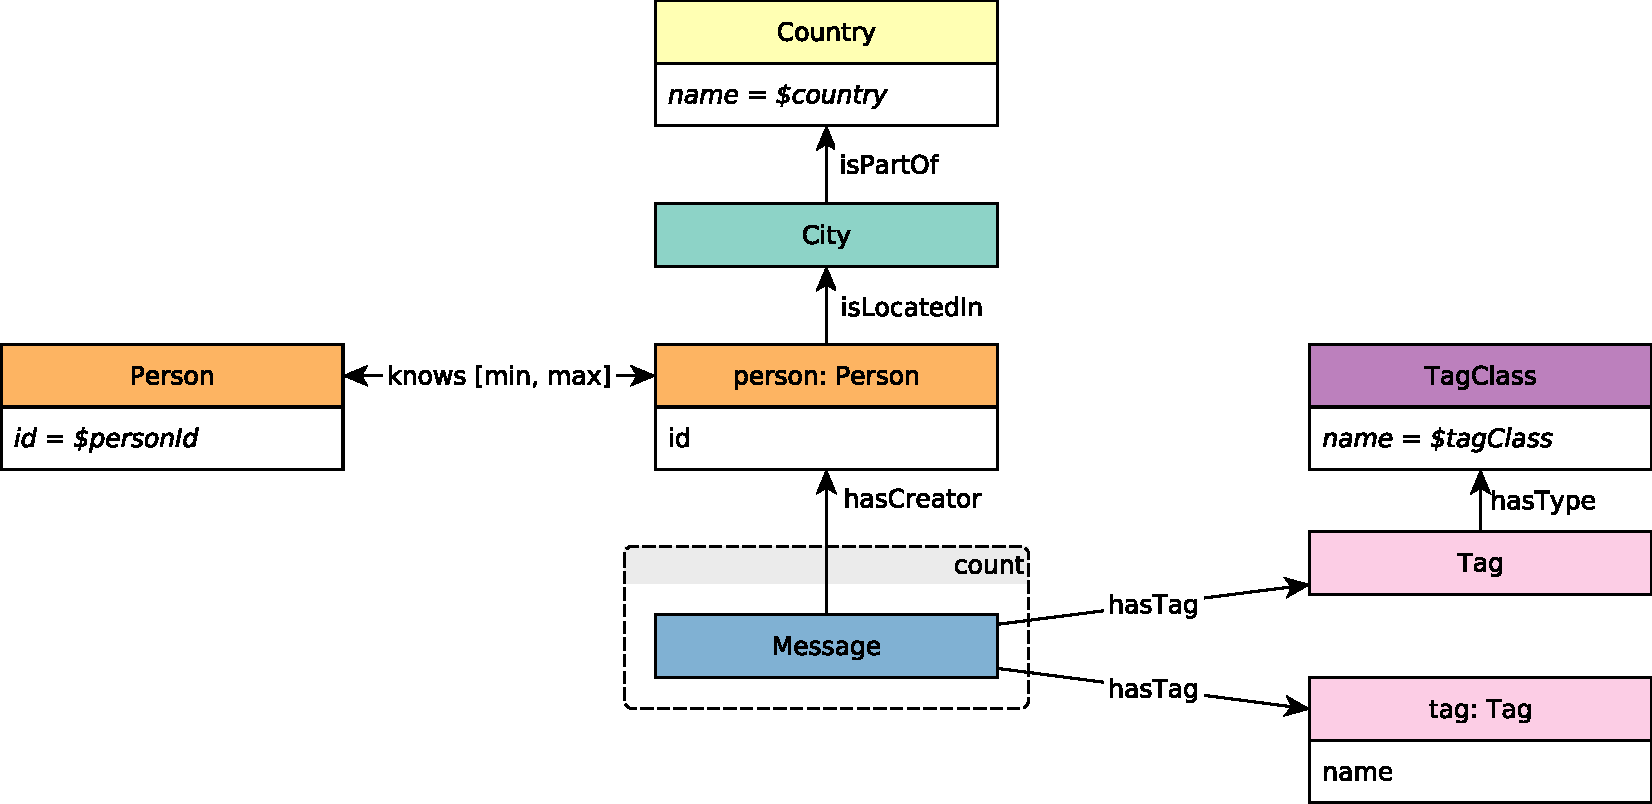
\includegraphics[scale=\patternscale,margin=0cm .2cm]{patterns/bi16}} \\ \hline
	description & Given a Person, find all other Persons that live in a given country and
are connected to given person by a transitive path with length in range
\texttt{{[}min,\ max{]}} through the knows relation.

{[}DISCUSS: edge isomorphism semantics{]}

For each of these Persons, retrieve all of their Messages (Posts \&
Comments) that contain at least one Tag belonging to a given TagClass
(direct relation not transitive).

For each Message, also retrieve its Tags.

TODO {[}szarnyasg{]}: what is postCount?
 \\ \hline
	
%
	group by       &
	\multicolumn{1}{>{\raggedright}X|}{
		\varname{tag.name}, 
		\varname{person.id}
		} \\ \hline
	
%
	parameters  &
	\vspace{1.1ex}{\begin{tabularx}{14.38cm}{|c|M|m{2cm}|Y} \hline
	\cellcolor{black!70} \color{white} $\mathsf{1}$ & \varname{personId} & \cellcolor{gray!20} \vartype{64-bit Integer} &  \\\hline
	\cellcolor{black!70} \color{white} $\mathsf{2}$ & \varname{country} & \cellcolor{gray!20} \vartype{String} &  \\\hline
	\cellcolor{black!70} \color{white} $\mathsf{3}$ & \varname{tagClass} & \cellcolor{gray!20} \vartype{String} &  \\\hline
	\cellcolor{black!70} \color{white} $\mathsf{4}$ & \varname{minPathDistance} & \cellcolor{gray!20} \vartype{32-bit Integer} &  \\\hline
	\cellcolor{black!70} \color{white} $\mathsf{5}$ & \varname{maxPathDistance} & \cellcolor{gray!20} \vartype{32-bit Integer} &  \\
	\end{tabularx}} \\ \hline
%
	result      &
	\vspace{1.1ex}{\begin{tabularx}{14.38cm}{|c|M|m{2cm}|Y} \hline
	\cellcolor{black!70} \color{white} $\mathsf{1}$ & \varname{person.id} & \cellcolor{gray!20} \vartype{64-bit Integer} &  \\\hline
	\cellcolor{black!70} \color{white} $\mathsf{2}$ & \varname{tag.name} & \cellcolor{gray!20} \vartype{String} &  \\\hline
	\cellcolor{black!70} \color{white} $\mathsf{3}$ & \varname{messageCount} & \cellcolor{gray!20} \vartype{32-bit Integer} & number of Messages created by that Person containing that Tag \\
	\end{tabularx}} \\ \hline
	%
	sort        &
	\vspace{1.1ex}{\begin{tabular}{|c|l|c|} \hline
	\cellcolor{black!70} \color{white} $\mathsf{1}$ & \varname{messageCount} & \cellcolor{gray!20} $\desc$ \\\hline
	\cellcolor{black!70} \color{white} $\mathsf{2}$ & \varname{tag.name} & \cellcolor{gray!20} $\asc$ \\\hline
	\cellcolor{black!70} \color{white} $\mathsf{3}$ & \varname{person.id} & \cellcolor{gray!20} $\asc$ \\
	\end{tabular}} \\ \hline
	%
	limit       & 100 \\ \hline
	%
	choke points &
	\multicolumn{1}{>{\raggedright}X|}{
		\chokepoint{1.2}, 
		\chokepoint{1.4}, 
		\chokepoint{2.3}, 
		\chokepoint{2.4}, 
		\chokepoint{3.3}, 
		\chokepoint{7.2}, 
		\chokepoint{7.3}
		}\\ \hline
\end{tabularx}
\clearpage
\renewcommand*{\arraystretch}{1.5}
\noindent\begin{tabularx}{17cm}{|p{1.95cm}|X|}
	\hline
	number      & 17                                                          \\ \hline
	title       & Friend triangles                                                           \\ \hline
	\multicolumn{2}{|c|}{ 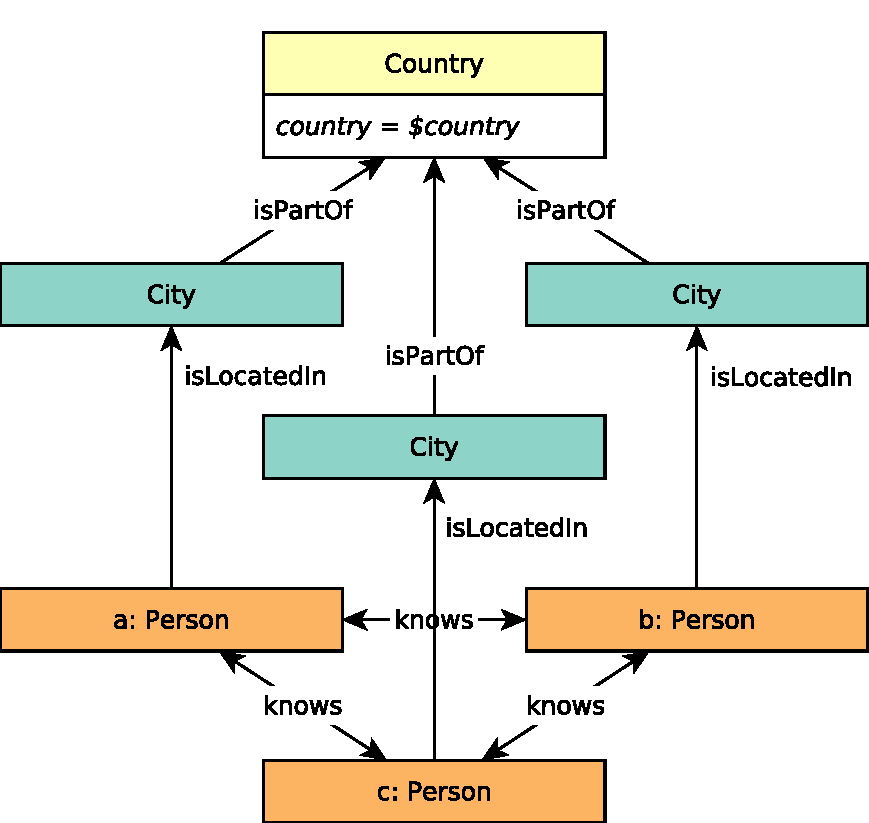
\includegraphics[scale=\patternscale,margin=0cm .2cm]{patterns/q17}} \\ \hline
	description & For a given country, count all the distinct triples of persons such that
\texttt{a} is friend of \texttt{b}, \texttt{b} is friend of \texttt{c},
and \texttt{c} is friend of \texttt{a}.

Distinct means that given a triple \emph{t1} in the result set \emph{R}
of all qualified triples, there is not a triple \emph{t2} in \emph{R}
such that \textbar{}\emph{t1} U \emph{b}\textbar{} = 3.
 \\ \hline
	
	parameters  &
	\renewcommand*{\arraystretch}{1.0}
	\vspace{-1.8ex}{\begin{tabularx}{14.2cm}{|c|l|p{2cm}|Y|} \hline
	\cellcolor{black!70} \color{white} $\mathsf{ 1 }$ & \varname{country} & \cellcolor{gray!20} \vartype{String} & \\ 
	\end{tabularx}} \\ \hline
	result      &
	\renewcommand*{\arraystretch}{1.0}
	\vspace{-1.8ex}{\begin{tabularx}{14.2cm}{|c|l|p{2cm}|Y|} \hline
	\cellcolor{black!70} \color{white} $\mathsf{ 1 }$ & \varname{count} & \cellcolor{gray!20} \vartype{32bitInteger} & \\ 
	\end{tabularx}} \\ \hline
	choke points        &
	\multicolumn{1}{>{\raggedright}X|}{
		\chokepoint{1.1}, 
		\chokepoint{2.3}
		}\\ \hline
\end{tabularx}
\clearpage
\renewcommand*{\arraystretch}{1.5}
\begin{tabularx}{15cm}{|p{2.1cm}@{\hskip 1ex}|@{\hskip 1ex}X|}
	\hline
	number      & 18                                                          \\ \hline
	title       & How many persons have a given number of posts                                                           \\ \hline
	\multicolumn{2}{|c|}{ 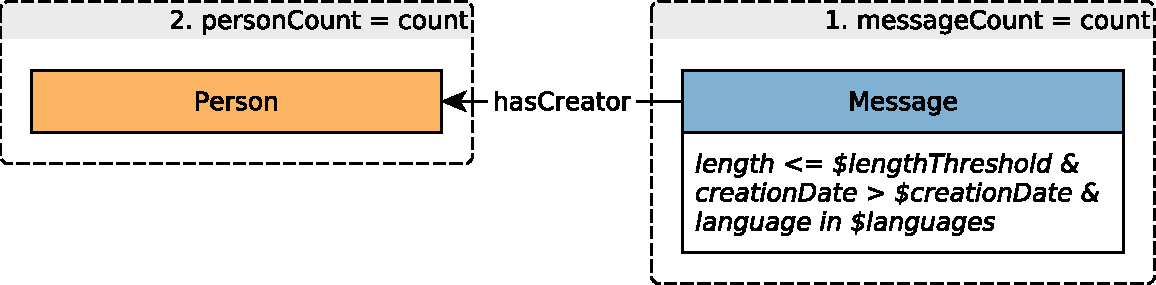
\includegraphics[scale=\patternscale,margin=0cm .2cm]{patterns/q18}} \\ \hline
	description & For each Person, count the number of Messages (Posts \& Comments) they
made.

Only consider messages with:

\begin{itemize}
\tightlist
\item
  length below the \texttt{lengthThreshold}
\item
  creationDate after \texttt{creationDate} (TODO - is after exclusive or
  inclusive, does it allow equality?)
\item
  any of the given \texttt{languages} (TODO - only Posts have a
  language, messages do not)
\end{itemize}
 \\ \hline
	
	group       &
	\multicolumn{1}{>{\raggedright}X|}{
		\varname{messageCount}
		}\\ \hline
	
	parameters  &
	\multicolumn{1}{>{\raggedright}X|}{
		\variable{creationDate}{Date} \\
		\variable{lengthThreshold}{TODO (32bitInteger?)} 
		}\\ \hline
	result      &
	\multicolumn{1}{>{\raggedright}X|}{
		\variable{messageCount}{32bitInteger}number of messages created\\
		\variable{personCount}{32bitInteger}the number of Persons with `messageCount` messages
		}\\ \hline
	sort        &
	\multicolumn{1}{>{\raggedright}X|}{
		\sortentry{personCount}{\desc}
		}\\ \hline
	choke points        &
	\multicolumn{1}{>{\raggedright}X|}{
		\chokepoint{1.1}, 
		\chokepoint{1.2}, 
		\chokepoint{1.6}, 
		\chokepoint{3.2}, 
		\chokepoint{4.2}, 
		\chokepoint{4.3}
		}\\ \hline
\end{tabularx}
\clearpage

\renewcommand*{\arraystretch}{1.1}

\noindent\begin{tabularx}{17cm}{|p{1.95cm}|X|}
	\hline
	workload    & BI \\ \hline
%
	query       & 19 \\ \hline
%
	title       & Stranger's interaction \\ \hline
%
    pattern     & \hfill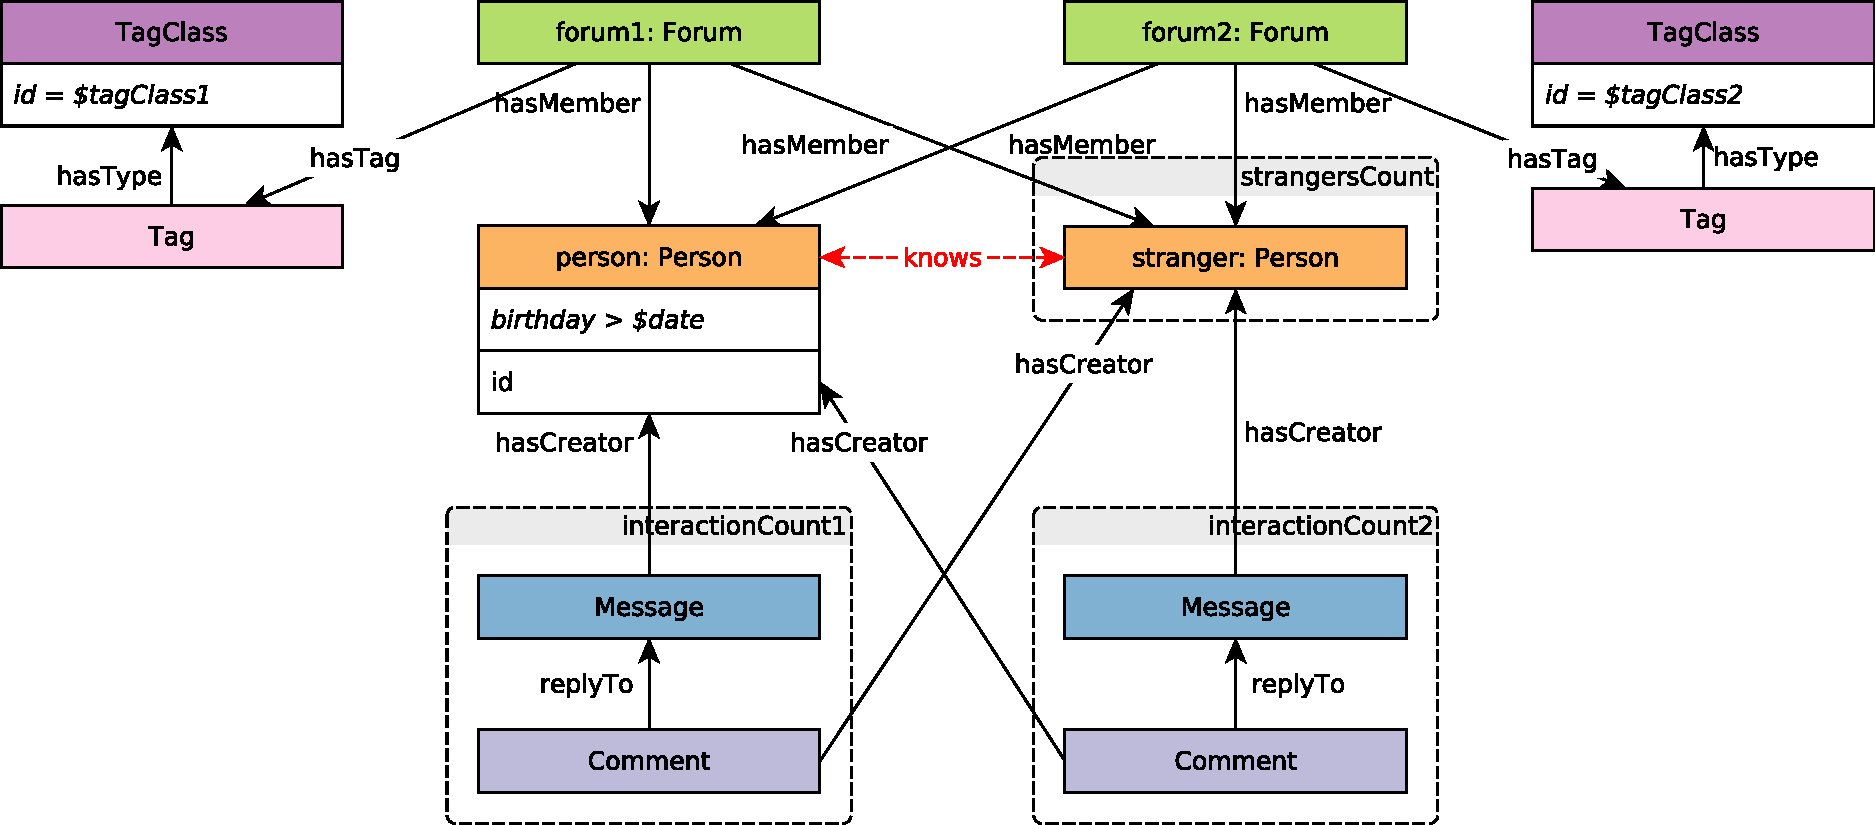
\includegraphics[scale=\patternscale,margin=0cm .2cm]{patterns/bi19}\hfill\vadjust{} \\ \hline
%
	description & For all the Persons born after a certain date, find all the strangers
they interacted with, where strangers are Persons that do not Know each
other. There is no restriction on the date that strangers were born.

Consider only strangers that are members of Forums tagged with tagClass1
(direct children not transitive) AND members of Forums tagged with
tagClass2 (direct children not transitive). It does not matter if these
Tags are attached to the same Forum, or different Forums.

We define interaction as follows: a Person replies to a Message (Post or
Comment) by another Person.

For each Person, count the number of strangers they interacted
(directed) with and total number of times they interacted (directed)
with them.
 \\ \hline
	
%
	parameters  &
	\vspace{1.1ex}{\begin{tabularx}{14.2cm}{|c|M|m{2cm}|Y|} \hline
	\cellcolor{black!70} \color{white} $\mathsf{1}$ & \varname{date} & \cellcolor{gray!20} \vartype{Date} &  \\ \hline
	\cellcolor{black!70} \color{white} $\mathsf{2}$ & \varname{tagClass1} & \cellcolor{gray!20} \vartype{32-bit Integer} &  \\ \hline
	\cellcolor{black!70} \color{white} $\mathsf{3}$ & \varname{tagClass2} & \cellcolor{gray!20} \vartype{32-bit Integer} &  \\ \hline
	\end{tabularx}}\vspace{1.1ex} \\ \hline
%
	result      &
	\vspace{1.1ex}{\begin{tabularx}{14.2cm}{|c|M|m{2cm}|Y|} \hline
	\cellcolor{black!70} \color{white} $\mathsf{1}$ & \varname{person.id} & \cellcolor{gray!20} \vartype{64-bit Integer} &  \\ \hline
	\cellcolor{black!70} \color{white} $\mathsf{2}$ & \varname{strangersCount} & \cellcolor{gray!20} \vartype{32-bit Integer} &  \\ \hline
	\cellcolor{black!70} \color{white} $\mathsf{3}$ & \varname{interactionCount} & \cellcolor{gray!20} \vartype{32-bit Integer} &  \\ \hline
	\end{tabularx}}\vspace{1.1ex} \\ \hline
	%
	sort        &
	\vspace{1.1ex}{\begin{tabular}{|c|l|c|} \hline
	\cellcolor{black!70} \color{white} $\mathsf{1}$ & \varname{interactionCount} & \cellcolor{gray!20} $\desc$ \\ \hline
	\cellcolor{black!70} \color{white} $\mathsf{2}$ & \varname{person.id} & \cellcolor{gray!20} $\asc$ \\ \hline
	\end{tabular}}\vspace{1.1ex} \\ \hline
	%
	limit       & 100 \\ \hline
	%
	choke points &
	\multicolumn{1}{>{\raggedright}X|}{
		\chokepoint{1.1}, 
		\chokepoint{1.4}, 
		\chokepoint{2.1}, 
		\chokepoint{2.3}, 
		\chokepoint{2.4}, 
		\chokepoint{3.3}, 
		\chokepoint{5.1}, 
		\chokepoint{7.3}, 
		\chokepoint{7.4}
		}\\ \hline
\end{tabularx}
\clearpage
\renewcommand*{\arraystretch}{1.1}

\noindent\begin{tabularx}{17cm}{|p{1.95cm}|X|}
	\hline
	number      & 20                                                          \\ \hline
%
	title       & High-level topics                                                           \\ \hline
	\multicolumn{2}{|c|}{ 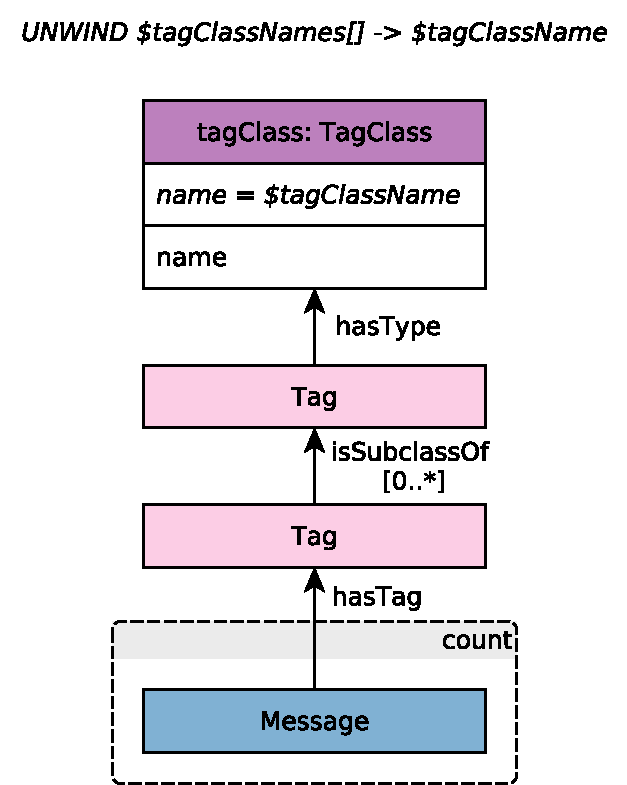
\includegraphics[scale=\patternscale,margin=0cm .2cm]{patterns/q20}} \\ \hline
	description & For all given TagClasses, count number of Messages that have a Tag that
belongs to that TagClass or any of its children (all descendants through
a transitive relation).
 \\ \hline
	
%
	parameters  &
	\vspace{1.1ex}{\begin{tabularx}{14.38cm}{|c|M|m{2cm}|Y} \hline
	\cellcolor{black!70} \color{white} $\mathsf{1}$ & \varname{tagClasses} & \cellcolor{gray!20} \vartype{String[]} &  \\
	\end{tabularx}} \\ \hline
%
	result      &
	\vspace{1.1ex}{\begin{tabularx}{14.38cm}{|c|M|m{2cm}|Y} \hline
	\cellcolor{black!70} \color{white} $\mathsf{1}$ & \varname{tagClass.name} & \cellcolor{gray!20} \vartype{String} & the TagClass of the root \\\hline
	\cellcolor{black!70} \color{white} $\mathsf{2}$ & \varname{postCount} & \cellcolor{gray!20} \vartype{32-bit Integer} &  \\
	\end{tabularx}} \\ \hline
	%
	sort        &
	\vspace{1.1ex}{\begin{tabular}{|c|l|c|} \hline
	\cellcolor{black!70} \color{white} $\mathsf{1}$ & \varname{postCount} & \cellcolor{gray!20} $\desc$ \\\hline
	\cellcolor{black!70} \color{white} $\mathsf{2}$ & \varname{tagClass.name} & \cellcolor{gray!20} $\asc$ \\
	\end{tabular}} \\ \hline
	%
	limit       & 100 \\ \hline
	%
	choke points &
	\multicolumn{1}{>{\raggedright}X|}{
		\chokepoint{1.6}, 
		\chokepoint{2.1}, 
		\chokepoint{6.1}
		}\\ \hline
\end{tabularx}
\clearpage
\renewcommand*{\arraystretch}{1.1}

\noindent\begin{tabularx}{17cm}{|p{1.95cm}|X|}
	\hline
	number      & 21                                                          \\ \hline
%
	title       & Zombies in a country                                                           \\ \hline
	\multicolumn{2}{|c|}{ \includegraphics[scale=\patternscale,margin=0cm .2cm]{patterns/q21}} \\ \hline
	description & Find zombies within the given country, and return their zombie scores.

A zombie is a Person created before the given \texttt{endDate} and that
has created between \texttt{{[}0,\ 1)} Messages per month, on average,
during the time range between profile creation date and the given
\texttt{endDate}.

The number of months spans the time range from creation date of the
profile to the \texttt{endDate} and also includes partial months.
 \\ \hline
	
%
	parameters  &
	\vspace{1.1ex}{\begin{tabularx}{14.2cm}{|c|l|m{2cm}|Y|} \hline
	\cellcolor{black!70} \color{white} $\mathsf{1}$ & \varname{country} & \cellcolor{gray!20} \vartype{String} &  \\\hline
	\cellcolor{black!70} \color{white} $\mathsf{2}$ & \varname{endDate} & \cellcolor{gray!20} \vartype{Date} &  \\
	\end{tabularx}} \\ \hline
%
	result      &
	\vspace{1.1ex}{\begin{tabularx}{14.2cm}{|c|l|m{2cm}|Y|} \hline
	\cellcolor{black!70} \color{white} $\mathsf{1}$ & \varname{person.id} & \cellcolor{gray!20} \vartype{64-bit Integer} &  \\\hline
	\cellcolor{black!70} \color{white} $\mathsf{2}$ & \varname{zombieLikeCount} & \cellcolor{gray!20} \vartype{32-bit Integer} &  \\\hline
	\cellcolor{black!70} \color{white} $\mathsf{3}$ & \varname{realLikeCount} & \cellcolor{gray!20} \vartype{32-bit Integer} &  \\\hline
	\cellcolor{black!70} \color{white} $\mathsf{4}$ & \varname{zombieScore} & \cellcolor{gray!20} \vartype{32bitFloat} & the ratio between the number of likes received from zombies (`zombieLikeCount`) and the total number of likes received on that person's messages (`realLikeCount`) -- only count likes received from profiles that were created before the given `endDate`. \\
	\end{tabularx}} \\ \hline
	%
	sort        &
	\vspace{1.1ex}{\begin{tabular}{|c|l|c|} \hline
	\cellcolor{black!70} \color{white} $\mathsf{1}$ & \varname{zombieScore} & \cellcolor{gray!20} $\desc$ \\\hline
	\cellcolor{black!70} \color{white} $\mathsf{2}$ & \varname{person.id} & \cellcolor{gray!20} $\asc$ \\
	\end{tabular}} \\ \hline
	%
	limit       & 100 \\ \hline
	%
	choke points &
	\multicolumn{1}{>{\raggedright}X|}{
		\chokepoint{1.2}, 
		\chokepoint{2.1}, 
		\chokepoint{2.3}, 
		\chokepoint{2.4}, 
		\chokepoint{3.2}, 
		\chokepoint{3.3}, 
		\chokepoint{5.1}, 
		\chokepoint{5.3}
		}\\ \hline
\end{tabularx}
\clearpage
\renewcommand*{\arraystretch}{1.1}

\noindent\begin{tabularx}{17cm}{|p{1.95cm}|X|}
	\hline
	number      & 22                                                          \\ \hline
%
	title       & International dialog                                                           \\ \hline
	\multicolumn{2}{|c|}{ \includegraphics[scale=\patternscale,margin=0cm .2cm]{patterns/q22}} \\ \hline
	description & Consider all pairs of people \texttt{(p1,\ p2)} such that one is located
in a city of Country \texttt{countryX} and the other is located in a
city of Country \texttt{countryY}.

For each city of Country \texttt{countryX}, return the highest scoring
pair.

The score of a pair is defined as the sum of the scores of the following
kinds of interaction:

\begin{itemize}
\tightlist
\item
  \texttt{p1} has created a reply Comment to at least one Comment or
  Post by \texttt{p2}: \texttt{Score\ =\ 4}
\item
  \texttt{p1} has created at least one Post or Comment that \texttt{p2}
  has created a reply Comment to: \texttt{Score\ =\ 1}
\item
  \texttt{p1} and \texttt{p2} Know each other: \texttt{Score\ =\ 15}
\item
  \texttt{p1} liked at least one Post or Comment by \texttt{p2}:
  \texttt{Score\ =\ 10}
\item
  \texttt{p1} has created at least one Post or Comment that was liked by
  \texttt{p2}: \texttt{Score\ =\ 1}
\end{itemize}

I.e., the maximum score a pair can obtain is:
\texttt{4\ +\ 1\ +\ 15\ +\ 10\ +\ 1\ =\ 31}
 \\ \hline
	
%
	parameters  &
	\vspace{1.1ex}{\begin{tabularx}{14.2cm}{|c|l|m{2cm}|Y|} \hline
	\cellcolor{black!70} \color{white} $\mathsf{1}$ & \varname{countryX} & \cellcolor{gray!20} \vartype{String} &  \\\hline
	\cellcolor{black!70} \color{white} $\mathsf{2}$ & \varname{countryY} & \cellcolor{gray!20} \vartype{String} &  \\
	\end{tabularx}} \\ \hline
%
	result      &
	\vspace{1.1ex}{\begin{tabularx}{14.2cm}{|c|l|m{2cm}|Y|} \hline
	\cellcolor{black!70} \color{white} $\mathsf{1}$ & \varname{p1.id} & \cellcolor{gray!20} \vartype{64-bit Integer} &  \\\hline
	\cellcolor{black!70} \color{white} $\mathsf{2}$ & \varname{p2.id} & \cellcolor{gray!20} \vartype{64-bit Integer} &  \\\hline
	\cellcolor{black!70} \color{white} $\mathsf{3}$ & \varname{cityX.name} & \cellcolor{gray!20} \vartype{String} &  \\\hline
	\cellcolor{black!70} \color{white} $\mathsf{4}$ & \varname{score} & \cellcolor{gray!20} \vartype{32-bit Integer} &  \\
	\end{tabularx}} \\ \hline
	%
	sort        &
	\vspace{1.1ex}{\begin{tabular}{|c|l|c|} \hline
	\cellcolor{black!70} \color{white} $\mathsf{1}$ & \varname{score} & \cellcolor{gray!20} $\desc$ \\\hline
	\cellcolor{black!70} \color{white} $\mathsf{2}$ & \varname{p1.id} & \cellcolor{gray!20} $\asc$ \\\hline
	\cellcolor{black!70} \color{white} $\mathsf{3}$ & \varname{p2.id} & \cellcolor{gray!20} $\asc$ \\
	\end{tabular}} \\ \hline
	%
	%
	choke points &
	\multicolumn{1}{>{\raggedright}X|}{
		\chokepoint{1.4}, 
		\chokepoint{1.6}, 
		\chokepoint{2.1}, 
		\chokepoint{3.1}, 
		\chokepoint{3.3}, 
		\chokepoint{5.1}, 
		\chokepoint{5.2}, 
		\chokepoint{5.3}
		}\\ \hline
\end{tabularx}
\clearpage
\renewcommand*{\arraystretch}{1.1}

\noindent\begin{tabularx}{17cm}{|p{1.95cm}|X|}
	\hline
	workload    & bi \\ \hline
%
	query       & 23 \\ \hline
%
	title       & Holiday destinations \\ \hline
	\multicolumn{2}{|c|}{ \includegraphics[scale=\patternscale,margin=0cm .2cm]{patterns/bi23}} \\ \hline
	description & Count the messages all residents of Country \texttt{country} have
written abroad grouped by month and Country. A Message was written
abroad if the Country the Message was written in is different than the
Country of the Person it was written by.
 \\ \hline
	
%
	parameters  &
	\vspace{1.1ex}{\begin{tabularx}{14.38cm}{|c|M|m{2cm}|Y} \hline
	\cellcolor{black!70} \color{white} $\mathsf{1}$ & \varname{country} & \cellcolor{gray!20} \vartype{String} &  \\
	\end{tabularx}} \\ \hline
%
	result      &
	\vspace{1.1ex}{\begin{tabularx}{14.38cm}{|c|M|m{2cm}|Y} \hline
	\cellcolor{black!70} \color{white} $\mathsf{1}$ & \varname{messageCount} & \cellcolor{gray!20} \vartype{32-bit Integer} & The number of messages in each group \\\hline
	\cellcolor{black!70} \color{white} $\mathsf{2}$ & \varname{country.name} & \cellcolor{gray!20} \vartype{String} & The name of the destination country \\\hline
	\cellcolor{black!70} \color{white} $\mathsf{3}$ & \varname{month} & \cellcolor{gray!20} \vartype{32-bit Integer} &  \\
	\end{tabularx}} \\ \hline
	%
	sort        &
	\vspace{1.1ex}{\begin{tabular}{|c|l|c|} \hline
	\cellcolor{black!70} \color{white} $\mathsf{1}$ & \varname{messageCount} & \cellcolor{gray!20} $\desc$ \\\hline
	\cellcolor{black!70} \color{white} $\mathsf{2}$ & \varname{country.name} & \cellcolor{gray!20} $\asc$ \\\hline
	\cellcolor{black!70} \color{white} $\mathsf{3}$ & \varname{month} & \cellcolor{gray!20} $\asc$ \\
	\end{tabular}} \\ \hline
	%
	limit       & 100 \\ \hline
	%
	choke points &
	\multicolumn{1}{>{\raggedright}X|}{
		\chokepoint{1.6}, 
		\chokepoint{2.3}, 
		\chokepoint{2.4}, 
		\chokepoint{3.3}, 
		\chokepoint{4.3}
		}\\ \hline
\end{tabularx}
\clearpage
\renewcommand*{\arraystretch}{1.1}

\noindent\begin{tabularx}{17cm}{|p{1.95cm}|X|}
	\hline
	workload    & bi \\ \hline
%
	query       & 24 \\ \hline
%
	title       & Messages by Topic and Continent \\ \hline
	\multicolumn{2}{|c|}{ \includegraphics[scale=\patternscale,margin=0cm .2cm]{patterns/bi24}} \\ \hline
	description & Find all Messages tagged with a Tag from the given TagClass
(non-transitive).

Count all messages and their likes grouped by continent, year, and
month. (TODO - do we group the Messages or the Persons who liked the
Messages by continent? I think the former one - szarnyasg)
 \\ \hline
	
%
	group by       &
	\multicolumn{1}{>{\raggedright}X|}{
		\varname{year}, 
		\varname{month}, 
		\varname{continent.name}
		} \\ \hline
	
%
	parameters  &
	\vspace{1.1ex}{\begin{tabularx}{14.38cm}{|c|M|m{2cm}|Y} \hline
	\cellcolor{black!70} \color{white} $\mathsf{1}$ & \varname{tagClass} & \cellcolor{gray!20} \vartype{String} &  \\
	\end{tabularx}} \\ \hline
%
	result      &
	\vspace{1.1ex}{\begin{tabularx}{14.38cm}{|c|M|m{2cm}|Y} \hline
	\cellcolor{black!70} \color{white} $\mathsf{1}$ & \varname{messageCount} & \cellcolor{gray!20} \vartype{32-bit Integer} &  \\\hline
	\cellcolor{black!70} \color{white} $\mathsf{2}$ & \varname{likeCount} & \cellcolor{gray!20} \vartype{32-bit Integer} &  \\\hline
	\cellcolor{black!70} \color{white} $\mathsf{3}$ & \varname{year} & \cellcolor{gray!20} \vartype{32-bit Integer} & year of the Message's creationDate \\\hline
	\cellcolor{black!70} \color{white} $\mathsf{4}$ & \varname{month} & \cellcolor{gray!20} \vartype{32-bit Integer} & month of the Message's creationDate \\\hline
	\cellcolor{black!70} \color{white} $\mathsf{5}$ & \varname{continent.name} & \cellcolor{gray!20} \vartype{String} &  \\
	\end{tabularx}} \\ \hline
	%
	sort        &
	\vspace{1.1ex}{\begin{tabular}{|c|l|c|} \hline
	\cellcolor{black!70} \color{white} $\mathsf{1}$ & \varname{year} & \cellcolor{gray!20} $\asc$ \\\hline
	\cellcolor{black!70} \color{white} $\mathsf{2}$ & \varname{month} & \cellcolor{gray!20} $\asc$ \\\hline
	\cellcolor{black!70} \color{white} $\mathsf{3}$ & \varname{continent.name} & \cellcolor{gray!20} $\desc$ \\
	\end{tabular}} \\ \hline
	%
	limit       & 100 \\ \hline
	%
	choke points &
	\multicolumn{1}{>{\raggedright}X|}{
		\chokepoint{1.6}, 
		\chokepoint{2.1}, 
		\chokepoint{2.3}, 
		\chokepoint{2.4}, 
		\chokepoint{3.2}, 
		\chokepoint{4.3}
		}\\ \hline
\end{tabularx}
\clearpage
\renewcommand*{\arraystretch}{1.1}

\noindent\begin{tabularx}{17cm}{|p{1.95cm}|X|}
	\hline
	number      & 25                                                          \\ \hline
%
	title       & Weighted paths                                                           \\ \hline
	\multicolumn{2}{|c|}{ \includegraphics[scale=\patternscale,margin=0cm .2cm]{patterns/q25}} \\ \hline
	description & Given two Persons, find all (unweighted) shortest paths between these
two Persons, in the subgraph induced by the Knows relationship.

Then, for each path calculate a weight. The nodes in the path are
Persons, and the weight of a path is the sum of weights between every
pair of consecutive Person nodes in the path.

The weight for a pair of Persons is calculated such that every reply (by
one of the Persons) to a Post (by the other Person) contributes 1.0, and
every reply (by ones of the Persons) to a Comment (by the other Person)
contributes 0.5.

Only consider messages that were created in a forum that was created
within the timeframe \texttt{{[}startDate,\ endDate{]}}.

Return all the paths with shortest length, and their weights.
 \\ \hline
	
%
	parameters  &
	\vspace{1.1ex}{\begin{tabularx}{14.2cm}{|c|l|m{2cm}|Y|} \hline
	\cellcolor{black!70} \color{white} $\mathsf{1}$ & \varname{person1Id} & \cellcolor{gray!20} \vartype{64bitInteger} &  \\\hline
	\cellcolor{black!70} \color{white} $\mathsf{2}$ & \varname{person2Id} & \cellcolor{gray!20} \vartype{64bitInteger} &  \\\hline
	\cellcolor{black!70} \color{white} $\mathsf{3}$ & \varname{startDate} & \cellcolor{gray!20} \vartype{Date} &  \\\hline
	\cellcolor{black!70} \color{white} $\mathsf{4}$ & \varname{endDate} & \cellcolor{gray!20} \vartype{Date} &  \\
	\end{tabularx}} \\ \hline
%
	result      &
	\vspace{1.1ex}{\begin{tabularx}{14.2cm}{|c|l|m{2cm}|Y|} \hline
	\cellcolor{black!70} \color{white} $\mathsf{1}$ & \varname{person.id} & \cellcolor{gray!20} \vartype{64bitInteger} & Identifiers representing an ordered sequence of the Persons in the path weight \\
	\end{tabularx}} \\ \hline
	%
	sort        &
	\vspace{1.1ex}{\begin{tabular}{|c|l|c|} \hline
	\cellcolor{black!70} \color{white} $\mathsf{1}$ & \varname{weight} & \cellcolor{gray!20} $\desc$ \\
	\end{tabular}} \\ \hline
	%
	%
	choke points &
	\multicolumn{1}{>{\raggedright}X|}{
		\chokepoint{1.2}, 
		\chokepoint{2.1}, 
		\chokepoint{2.2}, 
		\chokepoint{2.4}, 
		\chokepoint{3.3}, 
		\chokepoint{5.1}, 
		\chokepoint{5.3}, 
		\chokepoint{7.2}, 
		\chokepoint{7.3}
		}\\ \hline
\end{tabularx}
\clearpage

